%\documentclass[defaultstyle,10pt,Helvetica,oneside]{istulthesis}
\documentclass[defaultstyle,10pt,Helvetica,twoside,openright]{resources/istutlthesis}

% #############################################################################
% Preamble for Thesis-MSc in English or Portuguese
% Required Packages and commands
% --> Please Choose the MAIN LANGUAGE for the Thesis in package BABEL (below)
% !TEX root = ./main.tex
% #############################################################################
% Thesis-MSc
% Version 4, August 2022
% BY: Prof. Rui Santos Cruz, rui.s.cruz@tecnico.ulisboa.pt
% #############################################################################
%
% -----------------------------------------------------------------------------
% PACKAGES ucs, utf8x, babel, iflang:
% -----------------------------------------------------------------------------
% The 'ucs' package provides support for using UTF-8 in LaTeX documents.
% However in most situations it is not required.
\usepackage{ucs}
% The 'utf8x' package contains support for using UTF-8 as input encoding.
\usepackage[utf8x]{inputenc}
% The 'babel' package may correct some hyphenation issues of LaTeX.
% Select your MAIN LANGUAGE for the Thesis with the 'main=' option.
\usepackage[main=english,portuguese]{babel}
% The 'iflang' package is used to help determine the language being used.
\usepackage{iflang}

% -----------------------------------------------------------------------------
% PACKAGE scrbase:
% -----------------------------------------------------------------------------
% The 'scrbase' package is used to help redefining document structure.
\usepackage{scrbase}
% -----------------------------------------------------------------------------
% PACKAGE mathtools, amsmath, amsthm, amssymb, amsfonts, nicefrac:
% -----------------------------------------------------------------------------
% These packages are typically required.
% Among many other things they add the possibility to put symbols in bold
% by using \boldsymbol (not \mathbf); defines additional fonts and symbols;
% adds the \eqref command for citing equations.
\usepackage{mathtools, amsmath, amsthm, amssymb, amsfonts}
\usepackage{nicefrac}
%
% -----------------------------------------------------------------------------
% PACKAGE tikz:
% -----------------------------------------------------------------------------
% Tikz  for creating graphics programmatically.
\usepackage{tikz}
\usetikzlibrary{shapes.geometric, arrows, positioning}
% -----------------------------------------------------------------------------
% PACKAGES array, booktabs, multirow, colortbl, spreadtab:
% -----------------------------------------------------------------------------
% These packages are most usefull for advanced tables.
% 'multirow' allows to join rows throuhg the command \multirow which works
% similarly with the command \multicolumn.
% The 'colortbl' package allows to color the table (foreground and background)
% The package 'booktabs' provide some additional commands to enhance
% the quality of tables
% The 'longtable' package is only required when tables extend beyond the length
% of one page, which typically does not happen and should be avoided
\usepackage{array}
\usepackage{booktabs}
\usepackage{multirow}
\usepackage{colortbl}
\usepackage{spreadtab}
\usepackage{longtable}
\usepackage{pdflscape}
\usepackage{float}
%
% -----------------------------------------------------------------------------
% PACKAGES graphicx, subfigure:
% -----------------------------------------------------------------------------
% The package 'graphicx' supports formats PNG and JPG.
% Package 'subfigure' allows to place figures within figures with own caption.
% For each of the subfigures use the command \subfigure.
\usepackage{graphicx}
\usepackage[hang,small,bf,tight]{subfigure}
%
% -----------------------------------------------------------------------------
% PACKAGE caption:
% -----------------------------------------------------------------------------
% The 'caption' package offers customization of captions in floating
% environments such figure and table
% \usepackage[hang,small,bf]{caption}
\usepackage[format=hang,labelfont=bf,font=small]{caption}
% the following customization adds vertical space between caption and the table
\captionsetup[table]{skip=10pt}
%
% -----------------------------------------------------------------------------
% PACKAGE algorithmic, algorithm, algorithm2e:
% -----------------------------------------------------------------------------
% These packages are required if you need to describe an algorithm.
% The preference is for using 'algorithm2e'
%\usepackage{algorithmic}
%\usepackage[chapter]{algorithm}
\usepackage[ruled,vlined,algochapter,norelsize,\languagename]{algorithm2e}
%
% -----------------------------------------------------------------------------
% PACKAGE listings
% -----------------------------------------------------------------------------
% These packages are required if you need to list code snippets.
\usepackage{listings}
% Nicely syntax highlighted m-code in LaTeX documents with stylefile mcode.sty
% http://www.mathworks.com/matlabcentral/fileexchange/8015-m-code-latex-package
\usepackage[numbered]{resources/mcode}
%
% -----------------------------------------------------------------------------
% Re-define listings captions and titles based on language.
\newcaptionname{portuguese}{\lstlistingname}{Listagem} % Listings CAPTIONS
\newcaptionname{portuguese}{\lstlistlistingname}{Listagens} % LIST of LISTINGS
%
% -----------------------------------------------------------------------------
% PACKAGE csquotes
% -----------------------------------------------------------------------------
% Quotation helper package
\usepackage{csquotes}
%
% -----------------------------------------------------------------------------
% PACKAGE todonotes
% -----------------------------------------------------------------------------
% Create TODO Notes in text
% The notes can be made invisible by just using the 'disable' option:
\usepackage[textwidth=2cm, textsize=small]{todonotes}
%\usepackage[textwidth=2cm, textsize=small, disable]{todonotes}
\setlength{\marginparwidth}{2cm}
%
% -----------------------------------------------------------------------------
% PACKAGE changes
% -----------------------------------------------------------------------------
% Track changes in document (changes in pdf preview).
%% Use "final" option to make all tracking markups invisible.
%\usepackage[authormarkup=superscript,authormarkuptext=id,markup=underlined,ulem={ULforem,normalbf},final]{changes}
\usepackage[authormarkup=superscript,authormarkuptext=id,markup=underlined,ulem={ULforem,normalbf}]{changes}
% commands:
% \added[id=xx]{text}
% \deleted[id=xx]{text}
% \replaced[id=xx]{deleted text}{added text}
% -----------------------------------------------------------------------------
% PACKAGES xcolor, color
% -----------------------------------------------------------------------------
% These packages are required for list code snippets.
\usepackage{xcolor}
\usepackage{color}
% The following special color definitions are used in the IST Thesis
\definecolor{forestgreen}{RGB}{34,139,34}
\definecolor{orangered}{RGB}{239,134,64}
\definecolor{lightred}{rgb}{1,0.4,0.5}
\definecolor{orange}{rgb}{1,0.45,0.13}
\definecolor{darkblue}{rgb}{0.0,0.0,0.6}
\definecolor{lightblue}{rgb}{0.1,0.57,0.7}
\definecolor{gray}{rgb}{0.4,0.4,0.4}
\definecolor{lightgray}{rgb}{0.95, 0.95, 0.95}
\definecolor{darkgray}{rgb}{0.4, 0.4, 0.4}
\definecolor{editorGray}{rgb}{0.95, 0.95, 0.95}
\definecolor{editorOcher}{rgb}{1, 0.5, 0} % #FF7F00 -> rgb(239, 169, 0)
\definecolor{chaptergrey}{rgb}{0.6,0.6,0.6}
\definecolor{editorGreen}{rgb}{0, 0.5, 0} % #007C00 -> rgb(0, 124, 0)
\definecolor{olive}{rgb}{0.17,0.59,0.20}
\definecolor{brown}{rgb}{0.69,0.31,0.31}
\definecolor{purple}{rgb}{0.38,0.18,0.81}
%
% -----------------------------------------------------------------------------
% PACKAGE setspace:
% ----------------------------------------------------------------------------
% Provides support for setting the spacing between lines in a document.
% Package options include single spacing, one half spacing, and double spacing.
% Alternatively the spacing can be changed as required with:
% \singlespacing, \onehalfspacing, and \doublespacing commands
\usepackage{setspace}
%
% -----------------------------------------------------------------------------
% PACKAGE paralist
% -----------------------------------------------------------------------------
% This package provides the 'inparaenum' environment for inline lists
\usepackage{paralist}
% usage:
% \begin{inparaenum}[(a)]
% \item bla
% \item bla, bla
% \end{inparaenum}
% -----------------------------------------------------------------------------
% PACKAGE cite:
% -----------------------------------------------------------------------------
% The 'cite' package will result in citation numbers being automatically
% sorted and properly "ranged". i.e.,
% [1], [2], [5]--[7], [9]
\usepackage{cite}
%
% -----------------------------------------------------------------------------
% PACKAGE acronym:
% -----------------------------------------------------------------------------
% The package 'acronym' garantees that all acronyms definitions are
% given at the first usage.
% IMPORTANT: do not use acronyms in titles/captions; otherwise the definition
% will appear on the table of contents.
\usepackage[printonlyused]{acronym}
%
% -----------------------------------------------------------------------------
% PACKAGE hyperref
% -----------------------------------------------------------------------------
% Set links for references and citations in document
\usepackage{hyperref}
% pre-configuration of hyperref
\hypersetup{ colorlinks=true,
             citecolor=cyan,
             linkcolor=darkgray,
             urlcolor=teal,
             breaklinks=true,
             bookmarksnumbered=true,
             bookmarksopen=true,
}
%
% -----------------------------------------------------------------------------
% PACKAGE url:
% -----------------------------------------------------------------------------
% Provides better support for handling and breaking URLs.
\usepackage{url}
%
% -----------------------------------------------------------------------------
% PACKAGE Cleveref:
% -----------------------------------------------------------------------------
% Clever Referencing of document parts
% use \Cref[], or \cref[] for referencing items (Figures, Tables, Algorythms,
% Equations, Chapters, Sections, etc. No need to write the Name of the item.
% Note: portuguese is supported through "brazilian" option
\usepackage[\IfLanguageName{english}{english}{brazilian}]{cleveref}
%
% -----------------------------------------------------------------------------
% PACKAGE enumitem:
% -----------------------------------------------------------------------------
%For enhanced enumeration of lists
%\usepackage{enumitem}
\usepackage[shortlabels]{enumitem}
\setlist[description]{leftmargin=\parindent,labelindent=\parindent,itemsep=1pt,parsep=0pt,topsep=0pt}
%
% -----------------------------------------------------------------------------
% PACKAGE glossaries-extra:
% -----------------------------------------------------------------------------
% Allows creating a list of terms with definitions for those terms
\usepackage[xindy,toc,nopostdot]{glossaries}
\usepackage{glossaries-extra}

% Special style to print trailing dots before locations list
\makeatletter
\newglossarystyle{mystyle}{%
  \setglossarystyle{altlist}%
  \renewenvironment{theglossary}{%
  \begin{description}[style=standard,labelindent=0pt,itemsep=5pt]%
  }%
  {\end{description}}
  \renewcommand*{\glossentry}[2]{%
    \item[\glsentryitem{##1}%
      \glstarget{##1}{\glossentryname{##1}}]%
      \mbox{}\par\nobreak\@afterheading
      \glossentrydesc{##1}\glspostdescription
      {\def\hfill{\hskip 25pt plus 3fill}\dotfill\mbox{ ##2}}%
  }%
  \renewcommand{\glsgroupskip}{}%
}
\makeatother
\setglossarystyle{mystyle}

\makeglossaries

\newglossaryentry{maths}
{
    name=mathematics,
    description={Mathematics is what mathematicians do}
}

\newglossaryentry{LaTeX}
{
    name=LaTeX,
    description={LaTeX It is a mark up language specially suited for scientific documents as it can correctly format documents with all the typographical rules}
}


\newglossaryentry{formula}
{
    name=formula,
    description={A mathematical expression}
}
\if 0
\fi

% #############################################################################
% GLOBAL FORMATTING OF THE THESIS DOCUMENT before using FANCY stuff
% Load Titlepage definition
\usepackage{resources/titlepage}

% Set paragraph counter to alphanumeric mode
% DO NOT CHANGE these lines, otherwise the document will not respect the Guide
\renewcommand{\theparagraph}{\Alph{paragraph}~--}
\hoffset 0in
\voffset 0in
\oddsidemargin 0 cm
\evensidemargin 0 cm
\marginparsep 0in
\topmargin -0.25cm
\textwidth 16 cm
\textheight 22.4 cm
\makeatletter
% package indentfirst says \let\@afterindentfalse\@afterindenttrue
% and we revert this modification, reinstating the original definitio
% of \@afterindentfalse
\def\@afterindentfalse{\let\if@afterindent\iffalse}
\makeatother
% -----------------------------------------------------------------------------
% PACKAGE fancyhdr:
% -----------------------------------------------------------------------------
% The fancyhdr macro package allows to customize page headers and footers.
\usepackage{fancyhdr}
\pagestyle{fancy}
\renewcommand{\chaptermark}[1]{\markboth{\thechapter.\ #1}{}}
\renewcommand{\sectionmark}[1]{\markright{\thesection\ #1}}
\fancyhf{}
%#########################################################
% Choose the positioning of the Page Number
% Only on the Center side [C]
\fancyfoot[C]{\bfseries\thepage}
% Only on the Right side [R]
%\fancyfoot[R]{\bfseries\thepage}
% In case of Double sided printing, numbers are printed on Left (even pages) and on Right (odd pages)
%\fancyfoot[LE,RO]{\bfseries\thepage}
%#########################################################
\renewcommand{\headrulewidth}{0.0pt}
\renewcommand{\footrulewidth}{0.0pt}
\addtolength{\headheight}{2pt} % make space for the rule

\fancypagestyle{plain}{%
   \renewcommand{\headrulewidth}{0pt} % and the line
   \renewcommand{\footrulewidth}{0pt}
}
\fancypagestyle{blank}{%
   \renewcommand{\headrulewidth}{0pt} % and the line
   \renewcommand{\footrulewidth}{0pt}
}
\fancypagestyle{abstract}{%
   \renewcommand{\headrulewidth}{0pt}
   \renewcommand{\footrulewidth}{0.0pt}
}
\fancypagestyle{document}{%
	\renewcommand{\headrulewidth}{0.5pt}
	\renewcommand{\footrulewidth}{0.5pt}
	\addtolength{\headheight}{2pt} % make space for the rule
}
\setcounter{secnumdepth} {5}
\setcounter{tocdepth} {5}
\renewcommand{\thesubsubsection}{\thesubsection.\Alph{subsubsection}}
\renewcommand{\subfigtopskip}{0.3 cm}
\renewcommand{\subfigbottomskip}{0.2 cm}
\renewcommand{\subfigcapskip}{0.3 cm}
\renewcommand{\subfigcapmargin}{0.2 cm}
%
% -----------------------------------------------------------------------------
% PACKAGE minitoc:
% -----------------------------------------------------------------------------
% Package 'minitoc' creates a mini-table of contents (a “minitoc”) at
% the beginning of each chapter of a document.
% This packages are required for the \fancychapter configuration
\usepackage{minitoc}
\setcounter{minitocdepth}{1}
\setlength{\mtcindent}{24pt}
\renewcommand{\mtcfont}{\small\rm}
\renewcommand{\mtcSfont}{\small\bf}
\renewcommand*{\kernafterminitoc}{\kern0.\baselineskip\kern0.ex}
\mtcselectlanguage{\languagename}
% Now prepare the MINITOC
\def\boxedverbatim{%
  \def\verbatim@processline{%
    {\setbox0=\hbox{\the\verbatim@line}%
    \hsize=\wd0 \the\verbatim@line\par}}%
  \@minipagetrue%%%DPC%%%
  \@tempswatrue%%%DPC%%%
  \setbox0=\vbox\bgroup\vspace*{0.2cm}\footnotesize\verbatim
}
\def\endboxedverbatim{%
  \endverbatim
  \unskip\setbox0=\lastbox %%%DPC%%%
  \hspace*{0.2cm}
  \vspace*{-0.2cm}
  \egroup
  \fbox{\box0}% <<<=== change here for centering,...
}
% Now prepare the CHAPTER Number
\newcommand*{\chapnumfont}{%
%   \usefont{T1}{\@defaultcnfont}{b}{n}\fontsize{100}{130}\selectfont%
  \usefont{T1}{pbk}{b}{n}
  \fontsize{150}{130}
  \selectfont
  \color{chaptergrey}
}
\makeatletter
\def\@makechapterhead#1{%
  \vspace*{50\p@}%
  {\parindent \z@ \raggedright \normalfont
    {\chapnumfont\ifnum \c@secnumdepth >\m@ne
%         \huge\bfseries \@chapapp\space \thechapter
        \raggedleft\bfseries \thechapter
        \par\nobreak
        \vskip 20\p@
    \fi}
    \interlinepenalty\@M
    {\raggedleft\Huge \bfseries #1\par\nobreak}
    \vskip 40\p@
  }}
\makeatother
% Now put it all together as a command \fancychapter
\newcommand{\fancychapter}[1]{\chapter{#1}\vfill\minitoc\pagebreak}
%
% #############################################################################
% ADDITIONAL COMMANDS AND CONFIGURATIONS
% #############################################################################
% This commmand allows to place horizontal lines with a custom width...
% replaces the standard hline command
\newcommand{\hlinew}[1]{%
  \noalign{\ifnum0=`}\fi\hrule \@height #1 \futurelet
   \reserved@a\@xhline}
%
% -----------------------------------------------------------------------------
% This command defines some marks... USEFUL FOR TABLES.
\def\Mark#1{\raisebox{0pt}[0pt][0pt]{\textsuperscript{\footnotesize\ensuremath{\ifcase#1\or *\or \dagger\or \ddagger\or%
    \mathsection\or \mathparagraph\or \|\or **\or \dagger\dagger%
    \or \ddagger\ddagger \else\textsuperscript{\expandafter\romannumeral#1}\fi}}}}
%


% -----------------------------------------------------------------------------
% The following configurations are used for LISTINGS of certain languages
\lstdefinestyle{XML} {
	language=XML,
	extendedchars=true,
	breaklines=true,
	breakatwhitespace=true,
	emph={},
	emphstyle=\color{red},
	basicstyle=\small,
	xleftmargin=17pt,
	columns=fullflexible,
	commentstyle=\color{gray}\upshape,
	morestring=[b][\color{brown}]",
	morecomment=[s]{<?}{?>},
	morecomment=[s][\color{forestgreen}]{<!--}{-->},
	keywordstyle=\color{orangered},
	stringstyle=\ttfamily\color{black},
	% stringstyle=\ttfamily\color{black}\normalfont,
	tagstyle=\color{blue},
	% tagstyle=\color{darkblue}\bf,
	morekeywords={asn,action,addrType,abilityNAT,audioSampleRate,audiChannels,,bandwidth,bitmapSize,bitRate,connection,codecs,concurrentLinks,dependency,duration,frameRate,from,height,ip,id,lang,mimeType,onlineTime,peerMode,port,priority,peerProtocol,property,release,to,tier,type,transactionID,url,uploadBWlevel,version,width},
	otherkeywords={attribute,xmlns,schemaLocation,PresentationType,availabilityStartTime,availabilityEndTime,minimumUpdatePeriod,minBufferTime,UpdateTime},
}
% ----------------------------------------------------------------------------
\lstdefinelanguage{Assembler}{
	morecomment=[l];,
	keywords={ADD,ADDC,SUB,SUBB,CMP,MUL,DIV,MOD,NEG,AND,OR,NOT,XOR,TEST,BIT,SET,EI,EI0,EI1,EI2,EI3,SETC,EDMA,CLR,DI,DI0,DI1,DI2,DI3,CLRC,SHR,SHL,SHRA,SHLA,ROR,ROL,RORC,ROLC,MOV,MOVB,MOVBS,MOVP,MOVL,MOVH,SWAP,PUSH,POP,JZ,JNZ,JN,JNN,JP,JNP,JC,JNC,JV,JNV,JEQ,JNE,JLT,JLE,JGT,JGE,JA,JAE,JB,JBE,JMP,CALL,CALLF,RET,RETF,SWE,RFE,NOP},
	morekeywords={EQU,TABLE,WORD,STRING,PLACE},
}
% ----------------------------------------------------------------------------
\lstdefinestyle{coloredASM}{
	language=Assembler,
	extendedchars=false,
	breaklines=true,
	tabsize=2,
	numberstyle=\tiny,
	numbers=left,
	breakatwhitespace=true,
	emph={},
	emphstyle=\color{red},
	fontadjust=true,
	basicstyle=\small\ttfamily,
	% basicstyle=\footnotesize\ttfamily,
	columns=fixed,
	xleftmargin=17pt,
	framexleftmargin=17pt,
	framexrightmargin=5pt,
	framexbottommargin=4pt,
	commentstyle=\color{forestgreen}\upshape,
	morestring=[b][\color{brown}]",
	keywordstyle=\color{darkblue},
	stringstyle=\ttfamily\color{black},
	literate={á}{{\'a}}1 {ã}{{\~a}}1 {â}{{\^a}}1 {é}{{\'e}}1 {É}{{\'E}}1 {ê}{{\^e}}1 {õ}{{\~o}}1 {ó}{{\'o}}1 {í}{{\'i}}1 {ç}{{\c{c}}}1 {Ç}{{\c{C}}}1,
}
% ----------------------------------------------------------------------------
\lstdefinelanguage{CSS}{
	sensitive=true,
	morecomment=[l]{//},
	morecomment=[s]{/*}{*/},
	morestring=[b]',
	morestring=[b]",
	alsoletter={:},
	alsodigit={-},
	keywords={color,background-image:,margin,padding,font,weight,display,position,top,left,right,bottom,list,style,border,size,white,space,min,width, transition:, transform:, transition-property, transition-duration, transition-timing-function}
}
% ----------------------------------------------------------------------------
% JavaScript
\lstdefinelanguage{JavaScript}{
	morecomment=[s]{/*}{*/},
	morecomment=[l]//,
	morestring=[b]",
	morestring=[b]',
	morekeywords={typeof, new, true, false, catch, function, return, null, catch, switch, var, if, in, while, do, else, case, break}
}
% ----------------------------------------------------------------------------
\lstdefinelanguage{HTML5}{
	language=html,
	sensitive=true,
	alsoletter={<>=-},
	morecomment=[s]{<!-}{-->},
	tag=[s],
	otherkeywords={
	% General
	>,
	% Standard tags
	<!DOCTYPE,
	</html, <html, <head, <title, </title, <style, </style, <link, </head, <meta, />,
	% body
	</body, <body,
	% Divs
	</div, <div, </div>,
	% Paragraphs
	</p, <p, </p>,
	% scripts
	</script, <script,
	% More tags...
	<canvas, /canvas>, <svg, <rect, <animateTransform, </rect>, </svg>, <video, <source, <iframe, </iframe>, </video>, <image, </image>, <header, </header, <article, </article},
	ndkeywords={
	% General
	=,
	% HTML attributes
	charset=, src=, id=, width=, height=, style=, type=, rel=, href=,
	% SVG attributes
	fill=, attributeName=, begin=, dur=, from=, to=, poster=, controls=, x=, y=, repeatCount=, xlink:href=,
	% properties
	margin:, padding:, background-image:, border:, top:, left:, position:, width:, height:, margin-top:, margin-bottom:, font-size:, line-height:,
	% CSS3 properties
	transform:, -moz-transform:, -webkit-transform:,
	animation:, -webkit-animation:,
	transition:,  transition-duration:, transition-property:, transition-timing-function:,
	}
}
% ----------------------------------------------------------------------------
\lstdefinestyle{htmlcssjs} {%
	% General design
	backgroundcolor=\color{editorGray},
		fontadjust=true,
	basicstyle=\small\ttfamily,
	frame=b,
	% line-numbers
	xleftmargin={0.75cm},
	numbers=left,
	stepnumber=1,
	firstnumber=1,
	numberfirstline=true,
	% Code design
	identifierstyle=\color{black},
	keywordstyle=\color{blue}\bfseries,
	ndkeywordstyle=\color{editorGreen}\bfseries,
	stringstyle=\color{editorOcher}\ttfamily,
	commentstyle=\color{brown}\ttfamily,
	% Code
	language=HTML5,
	alsolanguage=JavaScript,
	alsodigit={.:;},
	tabsize=2,
	showtabs=false,
	showspaces=false,
	showstringspaces=false,
	extendedchars=true,
	breaklines=true,
	% German umlauts
	literate=%
	{Ö}{{\"O}}1
	{Ä}{{\"A}}1
	{Ü}{{\"U}}1
	{ß}{{\ss}}1
	{ü}{{\"u}}1
	{ä}{{\"a}}1
	{ö}{{\"o}}1
}
% ----------------------------------------------------------------------------
\lstdefinestyle{py} {%
	language=python,
	literate=%
	*{0}{{{\color{lightred}0}}}1
	{1}{{{\color{lightred}1}}}1
	{2}{{{\color{lightred}2}}}1
	{3}{{{\color{lightred}3}}}1
	{4}{{{\color{lightred}4}}}1
	{5}{{{\color{lightred}5}}}1
	{6}{{{\color{lightred}6}}}1
	{7}{{{\color{lightred}7}}}1
	{8}{{{\color{lightred}8}}}1
	{9}{{{\color{lightred}9}}}1,
	basicstyle=\small\ttfamily,
	numbers=left,
	% numberstyle=\tiny,
	% stepnumber=2,
	numbersep=5pt,
	tabsize=4,
	extendedchars=true,
	breaklines=true,
	keywordstyle=\color{blue}\bfseries,
	frame=b,
	commentstyle=\color{brown}\itshape,
	stringstyle=\color{editorOcher}\ttfamily,
	showspaces=false,
	showtabs=false,
	xleftmargin=17pt,
	framexleftmargin=17pt,
	framexrightmargin=5pt,
	framexbottommargin=4pt,
	backgroundcolor=\color{lightgray},
	showstringspaces=false,
}

\usepackage{
    amsmath,
    tabto,
}

\newtheorem{property}{Property}
\newtheorem{theorem}{Theorem}
\newtheorem{lemma}{Lemma}
\newtheorem{dem}{Proof}
\newcommand{\lArg}[1]{{\it #1}\xspace}
\newcommand{\nArg}[1]{{\rm{#1}}}
\newcommand{\eq}{$\leftarrow$}
\newcommand{\sysC}[1]{{#1}}


\begin{document}

\ifnum 1>0
\newcommand{\pd}[1]{\textit{\textcolor{red}{[Peter]: #1}}}
\newcommand{\bsd}[1]{\textit{\textcolor{red}{[Baltasar]: #1}}}
\newcommand{\rr}[1]{\textit{\textcolor{red}{[Rodrigo]: #1}}}
\definecolor{aoe}{rgb}{0.0, 0.5, 0.0}
\newcommand{\update}[1]{{\color{aoe}#1}}
\newcommand{\new}[1]{{\color{blue}#1}}
\else
\newcommand{\pd}[1]{}
\newcommand{\bsd}[1]{}
\newcommand{\rr}[1]{}
\newcommand{\update}[1]{}
\newcommand{\new}[1]{}
\fi

\pdfbookmark[0]{Titlepage}{Title}
% #############################################################################
% DEFINE THE Front Cover Page of Thesis-MSc
% !TEX root = ./main.tex
% #############################################################################
% Thesis-MSc
% Version 4, August 2022
% BY: Prof. Rui Santos Cruz, rui.s.cruz@tecnico.ulisboa.pt
% #############################################################################
%
% REQUIRED LOGO:
% The university logo image: arguments correspond to {left}{top} position.
% IST rules determine the position to be be 2cm from top, left page edge
\univlogo{20mm}{20mm}{img/ist_logo}
% OPTIONAL IMAGE:
% The thesis image: arguments are the start position in the page.
% You can change the image for your thesis, replacing the image name.
% If no image is desired, just comment the command
\thesislogo{25mm}{50mm}{img/thesis_logo}
%
% -----------------------------------------------------------------------------
% REQUIRED: Thesis TITLE
\title{Restart-Rollback: A Fault model for distributed systems
with persistent state}
% OPTIONAL: Thesis SUBTITLE
\subtitle{}
%
% -----------------------------------------------------------------------------
% REQUIRED: Author
% Author full Name
\author{Baltasar Azevedo e Silva Dinis}
%
% -----------------------------------------------------------------------------
% The official name of the course/degree. Please chose portuguese or english
% un-comment the line corresponding to your degree.
% You can add a degree name using thie following construct:
%
\degree{Information Systems and Computer Engineering}
%\degree{Engenharia Informática e de Computadores}
%\degree{Telecommunications and Informatics Engineering}
%\degree{Engenharia de Telecomunicações e Informática}
%
% -----------------------------------------------------------------------------
% REQUIRED: The SUPERVISOR(s) - maximum of two
\supervisor{Prof. Rodrigo Rodrigues}
% If no co-Supervisor comment the next line
\othersupervisor{Prof. Peter Druschel}
%
% -----------------------------------------------------------------------------
% REQUIRED: Date of examination
% Insert the Date of the Thesis discussion (format is MONTH and YEAR)
\date{November 2022}
%
% -----------------------------------------------------------------------------
% The following command define the author colors for Tracking Changes in doc in case you use Tracking
% the Two letters identify each author
\definechangesauthor[color=forestgreen]{MN}
\definechangesauthor[color=blue]{JO}
\definechangesauthor[color=red]{PT}

% -----------------------------------------------------------------------------
% Select 'false' when delivering the draft version of the thesis.
% The committee members should not be printed for the draft version.
% Select 'true' after the Examination Committee has accepted the thesis as final
\finalthesis{true}
%\finalthesis{false}
%
% -----------------------------------------------------------------------------
% The members of the Examination Committee
% Normally there is only the "vogalone"
% Comment the other if not necessary
\chairperson{TBD}
\vogalone{Prof. Nuno Santos}
%\vogaltwo{Dr. Name of Second Committee Member}
%\vogalthree{Eng. Name of Third Committee Member}
%
% -----------------------------------------------------------------------------
% The second page should be white with the Copyright message.

\maketitle
\thispagestyle{empty}
\cleardoublepage{}

\setcounter{page}{1} \pagenumbering{roman}
\baselineskip 18pt  % line spacing: -12pt for single spacing
                   %               -18pt for 1 1/2 spacing
                   %               -24pt for double spacing
\pdfbookmark[0]{Acknowledgments}{acknowledgments}
\begin{acknowledgments}
	% #############################################################################
% Agradecimentos / Acknowledgments
% !TEX root = ../main.tex
% #############################################################################

Acknowledgements

\end{acknowledgments}

\begin{abstract}
	% #############################################################################
% Abstract Text
% !TEX root = ../main.tex
% #############################################################################
% reset acronyms
\acresetall
% use \noindent in firts paragraph

\bsd{this is 279 words}
\noindent \acfp{TEE} ensure the confidentiality and integrity of
computations in hardware. Subject to the \ac{TEE}'s threat model,
the hardware shields a computation from most externally induced
fault behavior except crashes. As a result, a \acs{CFT}
replication protocol should be sufficient when replicating
trusted code inside \acp{TEE}. However, \acp{TEE} do not offer
efficient means of ensuring the freshness of persistent state,
which can be rolled back to an earlier version. In this
dissertation, we propose the \acf{RR} fault model for replicating
\acp{TEE}, which precisely captures the possible fault behaviors
of \acp{TEE} with external state, making it possible to avoid
using expensive \acs{BFT} protocols. Then, we show that existing
\acs{CFT} replication protocols can be easily adapted to this fault model
with few changes, while retaining their original performance.

\noindent We showcase the generality of the \ac{RR} model,
by applying it to the context of replicated \acsp{KVS}.
Current replicated \acsp{KVS} make a tradeoff
between latency, throughput and durability, depending on whether
they flush writes before replying (which offers poor
performance) or batch writes in memory (possibly losing data if
nodes crash before flushing). We observe that the latter case effectively
constitutes a rollback on restart and as such can be handled
using the \ac{RR} model.

\noindent We have verified our approach by implementing \ac{RR}
adaptations of two distributed protocols and compared
them experimentally with their \acs{CFT} and \acs{BFT}
counterparts. Furthermore, we
leverage these protocols to build two systems: replicated metadata service called
\acs{TEEMS}, and then show that it can be used to add \ac{TEE}-grade
confidentiality, integrity, and freshness to untrusted cloud storage
services; and \acs{R2-S2}, a replicated \acs{KVS}
which leverages the \ac{RR} model to achieve a middle ground between latency,
throughput and durability.

\bsd{ what i'd like, but there is a limit of 250 words}

\noindent \acfp{TEE} ensure the confidentiality and
integrity of computations in hardware. Subject to the \ac{TEE}'s threat
model, the hardware shields a computation from most externally induced
fault behavior except crashes. As a result, a \acf{CFT} replication protocol should be sufficient when replicating
trusted code inside \acp{TEE}.  However, \acp{TEE} do not provide efficient and
general means of ensuring the freshness of external, persistent
state. Therefore, \ac{CFT} replication is insufficient for
\ac{TEE} computations
with external state, as this state could be rolled back to an earlier
version when a \ac{TEE} restarts.  Furthermore, using \acf{BFT} protocols in this
setting is too conservative, because these protocols are designed to
tolerate arbitrary behavior, not just roll-back during a restart.

\noindent In this dissertation, we propose the \acf{RR} fault
model for replicating \acp{TEE}, which precisely captures the possible
fault behaviors of \acp{TEE} with external state. Then, we show that
existing replication protocols can be easily adapted to this fault
model with few changes, while retaining their original performance.
We adapted two widely used crash fault tolerant protocols~---~the
\acs{ABD}~\cite{abd} read/write register protocol and the Paxos~\cite{paxos}
consensus protocol~---~to the \ac{RR} model.  Furthermore, we
leverage these protocols to build a replicated metadata service called
\ac{TEEMS}, and then show that it can be used to add \ac{TEE}-grade
confidentiality, integrity, and freshness to untrusted cloud storage
services.  Our evaluation shows that our protocols perform
significantly better than their BFT counterparts (between $1.25$ and
$55\times$ better throughput), while performing identically to
the \ac{CFT} versions, which do not protect against rollback attacks.

\new{
\noindent We showcase the generality of the \ac{RR} model,
by applying it to the context of replicated \acp{KVS}.
Replicated \acp{KVS} typically have to make a tradeoff
between latency, throughput and durability. They either: 1)
synchronize incoming writes immediately, preventing
\emph{batching} and degrading
\emph{throughput}; 2) batch writes and wait for them to be
flushed, increasing the \emph{latency}; or 3) batch writes
and flush them in the background, risking losing the most recent updates if the node
crashes before the batch is flushed, compromising
\emph{durability}. We observe that this last option effectively
constitutes a rollback on restart and as such can be handled
using the \ac{RR} model. Based on this observation, we have
designed and implemented \ac{R2-S2}, a replicated \ac{KVS}
based on LevelDB which explores this
concept to achieve a middle ground between latency,
throughput and durability.
}

\end{abstract}

\begin{keywords}
	% #############################################################################
% English Keywords
% !TEX root = ../main.tex
% #############################################################################
% reset acronyms
\acresetall
% use \noindent in firts paragraph
\noindent TODO

\end{keywords}
\clearpage

\thispagestyle{empty}

\cleardoublepage{}

\begin{resumo}
	% #############################################################################
% RESUMO em Português
% !TEX root = ../main.tex
% #############################################################################
% use \noindent in firts paragraph
% reset acronyms
\acresetall
\noindent Ambientes de Execução Confiável (em inglês, TEEs)
garantem a confidencialidade e integridade de computações ao
nível do \textit{hardware}. Sobre o modelo adversarial dos TEEs, o
\textit{hardware} protege a computação da maioria das falhas
induzidas externamente, excepto falhas de \textit{crash}, em que
um TEE simplesmente vai abaixo (e.g., quando falta a
eletricidade). Contudo, TEEs, não possuem métodos eficientes de
garantir a frescura do seu estado persistente, que pode ser
revertido para uma versão anterior. Nesta dissertação, propomos o
modelo de faltas \ac{RR} para replicação de TEEs, que captura
exatamente os comportamentos de falta de TEEs com estado externo,
evitando a utilização de protocolos BFT, que incorrem num custo
superior. Mostramos que protocolos CFT existentes podem ser
adaptados facilmente para este modelo de faltas com poucas
alterações, mantendo a sua performance original.
\vskip -0cm
Para ilustrar a utilidade da replicação de TEEs segundo o
modelo RR, construímos um serviço de metadados replicado chamado
TEEMS, que pode ser usado para acrescentar confidencialidade,
integridade e frescura a armazenamento em cloud ao nível das
proteções dos TEEs. Seguidamente, exemplificamos a generalidade
do modelo RR, aplicando-o ao contexto de KVSs replicadas. KVSs
replicadas atuais escolhem entre latência, \textit{throughput} e
durabilidade, dependendo se sincronizam as escritas antes de
responderem aos pedidos (o que oferece uma \textit{performance}
fraca) ou se combinam várias escritas numa \textit{batch} em
memória (possivelmente perdendo dados se os nós forem abaixo
antes da escrita ser sincronizada). Observamos que o último
caso efetivamente corresponde a uma reversão de estado, que é
capturada pelo modelo RR.
\vskip 0cm
Impelmentámos os vários protocolos e sistemas, e a nossa
avaliação demonstra que a \textit{performance} é comparável à de
sistemas CFT mas com garantias mais fortes e significativamente
superior à de sistemas BFT.

\end{resumo}
\begin{palavraschave}
	% #############################################################################
% Portuguese Keywords
% !TEX root = ../main.tex
% #############################################################################
% reset acronyms
\acresetall
% use \noindent in firts paragraph

\noindent TODO

\end{palavraschave}
\clearpage

\thispagestyle{empty}

% This is required for the Fancy Chapters with minitoc
\dominitoc{}
\dominilof{}
\dominilot{}

\renewcommand{\baselinestretch}{1}
\pdfbookmark[0]{Contents}{toc}
\tableofcontents
\cleardoublepage{}

% reposition baseline
\renewcommand{\baselinestretch}{1.5}

\pdfbookmark[1]{List of Figures}{lof}
\listoffigures
\cleardoublepage{}
\begingroup
    % \let\clearpage\relax
    % \let\cleardoublepage\relax
    % \let\cleardoublepage\relax
% List of Tables
\pdfbookmark[1]{List of Tables}{lot}
\listoftables
\cleardoublepage{}

\pdfbookmark[1]{List of Algorithms}{loa}
\listofalgorithms{}
\endgroup
\cleardoublepage{}

\pdfbookmark[1]{Listings}{lol}
\lstlistoflistings{}
\cleardoublepage{}
% -----------------------------------------------------------------------------
% % List of acronyms
\pdfbookmark[1]{Acronyms}{loac}
\chapter*{\tlangAcronyms}
% #############################################################################
% This is the ACRONYMS Definition
% !TEX root = ../main.tex
% #############################################################################
% Do not forget to reorder Alphabetically the ACRONYMS !!!
% If there are special cases for Plural form see example hereunder
\begin{acronym}[H.264/SVC]
    \acro{ABD}{Attiya, Bar-Noy, Dolev}
	\acro{BFT}{Byzantine Fault Tolerant}
	\acro{CFT}{Crash Fault Tolerant}
	\acro{KVS}{Key-Value Store}
	\acro{LSM-tree}{Log-structured merge-tree}
	\acro{TEE}{Trusted Execution Environment}
	\acro{OS}{Operating System}
	\acro{R2-S2}{Restart-Rollback Storage System}
	\acro{RR}{Restart-Rollback}
    \acro{SMR}{state machine replication}
	\acro{TEE}{Trusted Execution Environment}
	\acro{TEEMS}{TEE Metadata System}
    \acro{YCSB}{Yahoo! Cloud Serving Benchmark}
\end{acronym}

\clearpage
\cleardoublepage{}
% -----------------------------------------------------------------------------

\setcounter{page}{1} \pagenumbering{arabic}
\baselineskip 18pt
% -----------------------------------------------------------------------------

\acresetall{}
\fancychapter{Introduction}\label{chap:intro}
\cleardoublepage{}

\bsd{\begin{enumerate}
    \item State of the Art: replicated systems with persistent
        state are treated akin to volatile state replicated
        systems, with the additional option of a node recovering
        from local state after restart;
    \item In certain security sensitive contexts, namely TEEs.
        this does not work. Nodes have limited control over
        persistent state, especially across restarts.
    \item To recover safely from persistent state one must use a
        stronger fault model. Currently, the only adequate model
        is BFT. This is far too strong, considering that nodes
        have correct and trusted execution.
    \item To bridge this gap, we develop the RR model, where
        a node's persistent state can be rolled back to a
        previous valid version. This way, TEEs can recover from
        their local persistent state.
    \item Taking a step back, this can be useful to extract
        performance from other replicated systems. In particular,
        by being more relaxed with syncronizing the volatile
        and persistent states, we can batch more aggressively.
        This would be otherwise unsafe, as a crash could rollback
        a replica.
    \item To evaluate our approach, we developed two systems,
        TEEMS and R2-S2. (Description of the systems and
        experimental results)
\end{enumerate}}

Replication is a standard technique in distributed systems, which adds
fault tolerance to a service implemented by an individual networked
node. To ensure that the replicated service appears to clients like
its single-node equivalent except for higher availability, a
replication protocol coordinates the replicated
nodes. For instance, to replicate a key value store \new{(i.e.:
a storage system which offers a simple get/put interface)} one can use the \ac{ABD}~\cite{abd}
protocol. For more complex applications that can be modelled
using a deterministic state machine, an \ac{SMR} protocol like
Paxos~\cite{paxos} may be used.

\new{Durability, i.e.\ not losing data even in the event of faults, is a key property of storage
systems. For replicated storage systems, adding local persistency
to the nodes that make up the system is a common practice. This
allows replicas to recover from crashes (in which they lose their
volatile state)} from their local \new{persistent} state, which in turn makes the
system resilient to catastrophic full system
shutdowns~\cite{bolosky:paxos}. From a
formal point of view, however, these systems are commonly treated in a
very similar fashion to others that store their state solely in
volatile memory. Indeed, when the persistent aspect of nodes
is explicitely considered, protocols are almost identical, with
small extensions that describe when and what data nodes need to
persist so that, in the event of a restart, the node can
operate as if nothing happened.

\new{This lack of explicit consideration of the persistent state
becomes a problem in certain security sensitive cases, in
particular in the context of \acp{TEE}. \acp{TEE} are
applications running in a special hardware-protected environment,
where the CPU shields the application, guaranteeing the integrity
and confidentiality of the code execution and the associated
volatile memory, in a way that it can be remotely attested that
the hardware protections were correctly set up. As such, they
have become an attractive solution for system administrators who
make deployments in infrastructure that they do not directly
control (e.g.\ the public cloud). \acp{TEE} run in an highly
adversarial attacker model, where the owner and operator of the
hardware is not trusted, and as such their control over the
persistent storage is quite limited, especially in the event of a
restart, where the \ac{TEE} cannot maintain records that ensure
the integrity and freshness of the persistent storage it is
using. Simply applying current replicated protocols would pose a
correctness and security problem.}\bsd{is this too vague? it is developed further down}

Despite these challenges, networked services implemented inside \acp{TEE} like
ARM TrustZone~\cite{armTZ}, AMD SEV-SNP~\cite{amdsev,
amdsev-snp}, Intel SGX~\cite{intelsgx}, or the future Intel
TDX~\cite{inteltdx} and ARM CCA~\cite{arm-cca} can similarly
benefit from replication.  Replicated \ac{TEE}-based systems aim
to combine the confidentiality, integrity, and remote attestation
of \acp{TEE} with replication to ensure high availability.
Examples include permissioned blockchains~\cite{teechain},
monotonic counters for ensuring state freshness~\cite{rote},
in-memory key-value stores~\cite{avocado-atc21}, as well as
broadcast and common random number generator
primitives~\cite{p2p-sgx}.

A key design decision in all replicated systems is the choice of fault
model underlying the replication protocol. This model captures the set
of faults that can affect an individual replica.  For instance, in the
{\em crash-fault model}, faulty nodes are assumed to execute correctly
until they crash at an arbitrary point in their execution, when they
seize to perform further steps until they restart. In the {\em
  Byzantine fault model}, faulty nodes may perform arbitrary
actions. The choice of fault model affects the complexity, overhead,
and tolerance threshold of a replication protocol, and is important
for both performance and security. A fault model that is too
pessimistic may lead to unnecessary safeguards, which can impact both
performance and the cost of replication. Conversely, a fault model
that is too optimistic may fail to account for all faults that can
occur, which then leads to broken assumptions and loss of correctness
or security of the replicated system.

In the case of \ac{TEE}-based replication, the choice of existing systems
that store replica state persistently~\cite{teechain,rote} was to
employ \ac{BFT} replication. This may seem
necessary given that rollback of persistent state is a behavior not
covered by the crash-fault model.  However, the Byzantine model is
much stronger than necessary for this setting. Intuitively, this
is because it assumes arbitrary behavior of
faulty components, thus not taking into account the integrity
guarantees for the code running inside \acp{TEE}.

To fill this gap in distributed replication research, we
introduce the \ac{RR} fault model, which
%is designed for replicated \ac{TEE}-isolated services and
captures precisely the set of faults that \acp{TEE} can suffer according to
their specification.  The main insight behind \ac{RR} is that,
apart from crash faults, whenever a \ac{TEE} restarts, the fault model
allows for a rollback of externally stored state to an earlier
version.  Such rollback events are possible because \acp{TEE} lack general
and high-performance means of ensuring the freshness of externally
stored state.  During an execution, however, the integrity of the
internal, volatile state of a \ac{TEE} is ensured by hardware, and the
integrity of any externally stored state can be ensured by standard
cryptographic means.

The \ac{RR} fault model occupies a middle ground between \ac{CFT}
and \ac{BFT}. As we will show, unlike CFT it provides
security for replicated \acp{TEE} by tolerating state roll-back at a cost
that is similar to \ac{CFT} and better than \ac{BFT}. Specifically, it is able
to substantially reduce the required communication, particularly for
read operations, in the common case where restarts are
infrequent.

Stepping back, we make the observation that the \ac{RR} fault
model can be useful, albeit for different reasons, in the more
general case of persistent replicated systems within the crash
model. A key factor for performance in this systems are the slow
accesses to untrusted storage, which must occur in the critical
path to ensure the correctness of the system. By batching
multiple requests together, it is possible to reduce this
overhead, increasing throughput at the expense of the additional
latency required to form the batch. Leveraging the \ac{RR} model,
it is possible to form batches more aggressively, replying to
certain requests before synchronizing to persistent storage. This
would otherwise be unsafe, as a crash before the synchronization
would constitute an effective rollback, which the \ac{RR} model
captures.

To demonstrate the potential of the \ac{RR} model, we apply it to
two types of replication protocols, namely the \ac{ABD}
 read/write replication protocol and the Paxos \ac{SMR}
protocol, showing that this adaptation is relatively straightforward.
We then use these protocols to devise two systems: \ac{TEEMS} and
\ac{R2-S2}. \ac{TEEMS}, a replicated metadata service,
is a relevant contribution in its own right, since
it enables Cloud storage with the same strong confidentiality and
integrity guarantees provided by \acp{TEE}. while also ensuring freshness
of data. \ac{TEEMS} is used with one or more untrusted cloud storage
services. \ac{TEEMS} maintains metadata for each data item (including the
encryption key, authentication code, latest version number and
policy), while ensuring strong security and enabling concurrent
sharing of data. \ac{R2-S2} is a replicated key value store built
using regular nodes (i.e. without TEEs or other security
mechanisms) that leverages the \ac{RR} model with the objective
of extracting higher throughput while retaining the strong reliability expected of a persistent
replicated system.

\section{Contributions}

In the \ac{TEE} context, we implemented the read/write
register and the \ac{SMR} protocols in three fault models:
\ac{CFT}, \ac{RR} and \ac{BFT}, and a prototype for \ac{TEEMS},
all using Intel SGX. In the storage context, we implemented
\ac{R2-S2} as a replication layer on top of a single node key
value store. We evaluated our prototypes using both
microbenchmarks and real-world workloads, namely
\ac{YCSB}~\cite{ycsb}.

Our contributions include:
\begin{enumerate}
    \item The \ac{RR} fault model, which is the first to capture
        precisely the fault behavior of \acp{TEE} that rely on external storage;
    \item A derivation of quorum sizes for replication protocols
        in the \ac{RR} model;
    \item Principles for the adaptation of \ac{CFT} protocols to
        the \ac{RR} model;
    \item Two protocols for this model, implementing read-write
        storage and \ac{SMR};
    \item The \ac{TEEMS} generic metadata service, and its integration with
        untrusted cloud storage services to give clients the ability to share
        and concurrently access persistent data with strong confidentiality,
        integrity, and freshness;
    \item The \ac{R2-S2} distributed key value store, which
        enables higher throughput from key value stores backed by
        persistent state;
    \item An extensive experimental evaluation of our protocols
        in the \ac{TEE} setting, with a \update{detailed} comparison with
        unsafe \ac{CFT} and expensive \ac{BFT} solutions;
    \item An experimental evaluation of the \ac{R2-S2}
        system.
\end{enumerate}


% #############################################################################
\section{Organization of the Document}

The rest of the thesis is organized as follows:
\Cref{chap:related} covers related work. In \cref{chap:model} we
formalize the \ac{RR} model and show the derivation of
\ac{RR}-based quorum systems and protocols. \Cref{chap:tee}
describes the usage of \acp{TEE} with \ac{RR}, with the
accompanying design and evaluation of \ac{TEEMS}. In
\cref{chap:storage} we present the design of
\ac{R2-S2} and its experimental evaluation.
\Cref{chap:conclusion} summarizes our work and presents possible
avenues for future work.

% #############################################################################

\if 0 % paper intro

Replication is a standard technique in distributed systems, which adds
fault tolerance to a service implemented by an individual networked
node. To ensure that the replicated service appears to clients like
its single-node equivalent except for higher availability, a
replication protocol coordinates the replicated
nodes. For instance, a state machine replication (SMR) protocol like
Paxos~\cite{paxos} may be used for this purpose.

Networked services implemented inside a trusted execution environment
(TEE) like ARM TrustZone~\cite{armTZ}, AMD SEV-SNP~\cite{amdsev,
  amdsev-snp}, Intel SGX~\cite{intelsgx}, or the future Intel
TDX~\cite{inteltdx} and ARM CCA~\cite{arm-cca} can similarly benefit
from replication.  Replicated \ac{TEE}-based systems aim to combine the
confidentiality, integrity, and remote attestation of \acp{TEE} with
replication to ensure high availability.
%and resilience to rollback attacks that revert the externally stored,
%persistent state of a TEE~\cite{memoir}
%\bsd{the reference to rollback attacks early on seems out of place,
%  since this is a gap in most replicated \acp{TEE}. Moreover, memoir is not
%  a replicated \ac{TEE} system}.
Examples include permissioned blockchains~\cite{teechain}, monotonic
counters for ensuring state freshness~\cite{rote}, in-memory key-value
stores~\cite{avocado-atc21}, as well as broadcast and common random
number generator primitives~\cite{p2p-sgx}.

A key design decision in all replicated systems is the choice of fault
model underlying the replication protocol. This model captures the set
of faults that can affect an individual replica.  For instance, in the
{\em crash-fault model}, faulty nodes are assumed to execute correctly
until they crash at an arbitrary point in their execution, when they
seize to perform further steps until they restart. In the {\em
  Byzantine fault model}, faulty nodes may perform arbitrary
actions. The choice of fault model affects the complexity, overhead,
and tolerance threshold of a replication protocol, and is important
for both performance and security. A fault model that is too
pessimistic may lead to unnecessary safeguards, which can impact both
performance and the cost of replication. Conversely, a fault model
that is too optimistic may fail to account for all faults that can
occur, which then leads to broken assumptions and loss of correctness
or security of the replicated system.

In the case of \ac{TEE}-based replication, the choice of existing systems
that store replica state persistently~\cite{teechain,rote} was to
employ Byzantine fault tolerant (BFT) replication. This may seem
necessary given that rollback of persistent state is a behavior not
covered by the crash-fault model.  However, the Byzantine model is
much stronger than necessary for this setting. Intuitively, this
is because it assumes arbitrary behavior of
faulty components, thus not taking into account the integrity
guarantees for the code running inside \acp{TEE}.

In this paper, we fill a gap in distributed replication research by
introducing the restart-rollback (\faultmodel) fault model, which
%is designed for replicated \ac{TEE}-isolated services and
captures precisely the set of faults that \acp{TEE} can suffer according to
their specification.  The main insight behind \faultmodel\ is that,
apart from crash faults, whenever a \ac{TEE} restarts, the fault model
allows for a rollback of externally stored state to an earlier
version.  Such rollback events are possible because \acp{TEE} lack general
and high-performance means of ensuring the freshness of externally
stored state.  During an execution, however, the integrity of the
internal, volatile state of a \ac{TEE} is ensured by hardware, and the
integrity of any externally stored state can be ensured by standard
cryptographic means.

The \faultmodel\ fault model occupies a middle ground between crash
fault tolerance (CFT) and BFT. As we will show, unlike CFT it provides
security for replicated \acp{TEE} by tolerating state roll-back at a cost
that is similar to CFT and better than BFT. Specifically, it is able
to substantially reduce the required communication, particularly for
read operations, in the common case where restarts are
infrequent.

To demonstrate the potential of the \faultmodel\ model, we apply it to
two types of replication protocols, namely the Attiya, Bar-Noy, Dolev
(ABD) read/write replication protocol and the Paxos
state machine replication (SMR)
protocol, showing that this adaptation is relatively straightforward.
%; and, we apply each protocol to a specific application scenario.
We then use these protocols to devise a replicated metadata service
called \sys, which is a relevant contribution in its own right, since
it enables Cloud storage with the same strong confidentiality and
integrity guarantees provided by \acp{TEE}. while also ensuring freshness
of data.
% and the ability to securely share data between clients by
% enforcing access policies. To this end, \sys\ provides a
% generic, scalable,
%\sys\ is a trustworthy metadata service hosted in a replicated set of
%TEEs, which may themselves be hosted by a diverse set of cloud
%providers for increased resilience.
%This service provides a semantically rich interface with
%persistent updates and read-modify-write (RMW) operations.
\sys\ is used with one or more untrusted cloud storage
services. \sys\ maintains metadata for each data item (including the
encryption key, authentication code, latest version number and
policy), while ensuring strong security and enabling concurrent
sharing of data.

%and updates this metadata and the respective data atomically using the simple read/write protocol for the \faultmodel\ model.\bsd{need to rewrite this, present that it uses both protocols}

%The second case study is inspired by permissioned blockchains, and
%their ability to improve performance by offloading transactions to a
%payment channel running a more efficient protocol, and then settling
%the final balance to the main blockchain. To support this, we built a
%state machine replication protocol based on the \faultmodel\ model,
%thus allowing the more complex operations of these payment channels to
%be supported in a resilient way.

We implemented both the read/write and SMR replication protocols for
three different fault models (\faultmodel, crash, and Byzantine), and
we also implemented \sys\ and used it to implement a new class of
secure cloud storage services. We evaluated the protocols using
microbenchmarks and the storage system using both microbenchmarks and
YCSB.  Our experimental results show that the protocols for the
\faultmodel\ model perform significantly better than their BFT
counterparts, and, compared to CFT, they perform identically while
additionally tolerating rollback attacks.
Furthermore, \sys\ offers secure, sharable storage at modest overhead.

Our contributions include:
%\begin{enumerate}
%\item
 (1) The \faultmodel\ fault model, which is the first to capture
precisely the fault behavior of \acp{TEE} that rely on external storage;
%    \item
(2) a derivation of quorum sizes for replication protocols in the
\faultmodel\ model;
      %     \item
(3) principles for the adaptation of CFT protocols to
the \faultmodel\ model;
%\item
(4) two protocols for this model, implementing read-write storage and
SMR;
        %    \item
(5) The \sys\ generic metadata service, and its integration with
untrusted cloud storage services to give clients the ability to share
and concurrently access persistent data with strong confidentiality,
integrity, and freshness;
%\item
(6) An extensive experimental evaluation of our protocol, and of the
storage solutions based on \sys\ in different deployment scenarios.
%\end{enumerate}


The remainder of the paper is organized as follows.  We motivate
our work and provide some background \S\ref{sec:fault_model},
describe the \faultmodel\ model in \S\ref{sec:model}, present the
replication protocols in the new model in
\S\ref{sec:protocol}, and an example application built using
those protocols in \S\ref{sec:metadata}.  We describe our
prototype implementations in \S\ref{sec:impl}, evaluate them
experimentally in \S\ref{sec:eval}, survey related work in
\S\ref{sec:related_work}, and conclude in \S\ref{sec:conclusion}.





\fi

\cleardoublepage{}

\fancychapter{Related Work}\label{chap:related}
\cleardoublepage{}

\section{Fault Models}\label{sec:related_fault_models}

In this section, we survey the most used classes of fault models
for distributed systems and compare them the novel
\ac{RR} model. It is important to first clarify that, both
here and in the rest of this document, we consider the network to
be asynchronous. This means that the upper bound for the message
delivery delay between replicas is unknown, and may not even
exist. This model is consistent with the Internet, where network
partitions may temporarily impede or arbitrarily slow down the
communication between two nodes.

\paragraph{Crash fault models.} A crash fault is said to have
occurred when a node stops replying to requests. This may happen
for several reasons: power outages, network
partitions, programming errors that
cause the processes to crash, etc. A crash fault can be
considered \emph{fail-stop} if other processes can detect that it
has in fact crashed. However, perfect failure detection in asynchronous
systems is impossible~\cite{perfect-failure-impossible}. A node that
suffers a crash fault is indistinguishable from an extremely slow
one~\cite{polynomial-communication} (rigourously, a node which replies at $t = \infty$).  The
\emph{crash-recovery}
model~\cite{consensus-recovery,crash-recovery} is a slight variation from the crash
model, wherein replicas are allowed to restart and run a recovery
protocol.

\paragraph{Byzantine fault models.}
First introduced by Lamport et al in~\cite{lamport:byzgenerals},
a Byzantine fault is the most encompassing type of fault
possible, since it assumes nodes can deviate arbitrarily from the
prescribed protocol. They may do so maliciously or simply by component
or programming error. Furthermore, several Byzantine nodes may
collude to deviate in a coordinated fashion, in an attempt to
subvert the guarantees of the system. Compared to crash fault
tolerant protocols, \ac{BFT} protocols are expensive on account of
mechanisms such as digital signatures~\cite{bqs} or extra protocol
rounds~\cite{pbft}.

\paragraph{Hybrid fault models.}
Hybrid fault models consider at least two types of faults
separately. They have the advantage of better adapting the
system parameterization to the deployment conditions by offering
greater flexibility, at the cost of some complexity.
UpRight~\cite{upright} is an example of a system which uses such
a hybrid fault model, concretely a hybrid crash-\ac{BFT} model, where
the system is able to sustain a different number of crash and
Byzantine faults. In particular, UpRight sustains $u$ crash faults in addition
to $r$ commission faults, which are a subset of Byzantine faults
where nodes actively produce an incorrect message (and thus
excluding the subset of crash faults from the Byzantine failure
model). This leads to an elegant reasoning about Byzantine fault
tolerance that separates incorrect from non-incorrect node
behavior.

Besides protocol changes, different fault models require
different quorum systems. A \emph{quorum} is defined as the
minimum set of replies that need to be gathered to proceed to the
next step of the protocol. The size of quorums is of great
importance for the economical cost of systems, as larger quorums require
more replicas and resources, as well as their performance, as
larger quorums will generally take longer to gather. These
quorums not only depend on the fault model, but on the network
model and synchrony assumptions. As an example,
Table~\ref{tab:quorum} has the quorum sizes for the crash,
Byzantine and UpRight models in the asynchronous model.

\begin{table}[ht]
    \centering
    \caption{Quorum sizes in different fault models. In the crash
    model $f$ is the number of crashed replicas, in the Byzantine
    model $f$ is the number of Byzantine replicas, and in the
    UpRight model $u$ is the number of crash faults and $r$
    the number of commission faults tolerated.}
    \begin{tabular}{|l|c|c|c|}
        \hline
        \textbf{Fault Model} & \textbf{Fault Parameter} & \textbf{\# Replicas} & \textbf{Quorum Size} \\
        \hline
        Crash & f & 2 f + 1 & f + 1 \\
        \hline
        Byzantine & f & 3 f + 1 & 2 f + 1 \\
        \hline
        UpRight & u, r & 2 u + r + 1 & u + r + 1 \\
        \hline
    \end{tabular}\label{tab:quorum}
\end{table}

\paragraph{Comparison to \ac{RR}.}
The \ac{RR} model allows for the system to tolerate a combination of
crash faults and faults where a replica has stale state after a
restart. The \ac{RR} model is strictly more encompassing than
the crash model, allowing for fault behaviors that are
not tolerated by this. Compared to \ac{BFT}, it does not need to
protect against generic Byzantine faults, leading to simpler,
more efficient protocols with smaller quorums in the common case.
Finally, compared to hybrid crash-\ac{BFT}
models~\cite{MeyerPradhan91,bc:hybrid,mc:hybrid,upright}, while
\ac{RR} is also a hybrid model, it differs in the type of
non-crash behavior it admits, since wrong answers in \ac{RR}
are limited to rollbacks after a restart, whereas previous hybrid
models tolerated arbitrary Byzantine faults.

The \ac{RR} model has some relevant characteristics such as
leading to dynamic quorum sizes, where the size depends on the
number of replies from recently restarted nodes, leading to small
read quorums in the normal case. Other proposals, such as Refined
Quorum Systems~\cite{rqs} or Flexible Paxos~\cite{fp},  also use
varying quorum sizes in different parts of the protocol. However,
they do it in a way that is complementary to ours, since they
work on traditional models (crash and Byzantine) and come up with
protocol techniques based on different quorum sizes to improve
performance. In contrast, \ac{RR} is a new model (based on a
different set of assumptions) that naturally leads to dynamic
quorums.

Another approach of hybrid quorums has been put forward by
\ac{VFT}~\cite{visigoth}. In \ac{VFT} not only are crash and
commission faults separately considered, the synchrony of the
system is also a parameter of the quorum system. This allows
\ac{VFT} to be parameterized as either synchronous or asynchronous
and as either crash or Byzantine, with hybrid combinations.
Although an interesting contribution, we consider \ac{VFT} to be
an orthogonal approach.

\section{Replication Protocols}
Replication is a technique wherein multiple copies of a service run
simultaneously so that the overall system maintains its operation
even in the presence of faults. There are several protocols for
replicated services, varying vastly according to the types of
faults tolerated, performance characteristics and semantics of
the service. In this section, we will survey two types of
services frequently replicated: read-write registers and state
machines.

\paragraph{Read-Write Register.} A read-write register supports a
very simple interface, allowing clients to either read the
current value or writing a new one. Due to their simplicity,
protocols for replicating registers are considered to be quite
fast. The ABD protocol proposed by Attiya
\emph{et al.}~\cite{abd} implements this register in the crash
model, while the Malkhi and Reiter proposed a Byzantine fault tolerant
counterpart in~\cite{bqs}.

\paragraph{State Machine Replication.} A deterministic state machine (SM) is a
mathematical construct that supports the successive application of
\emph{operations}, which mutate its internal state. This is a
powerful programming abstraction, as it can simulate any
deterministic computation. For that reason, it has been the
object of much research within the distributed systems community:
using state machine replication (SMR), system builders can build
arbitrarily complex fault tolerant systems~\cite{schneider-smr} (provided that they
are deterministic). A common method for achieving SMR is to
attach a \emph{consensus} module to an operation log. Consensus
is a process by which a set of nodes agree on a value. By agreeing
on the value for each entry in the log, replicas can then be sure
that they apply the same operations to their local state machines in the same order,
guaranteeing that their state is consistent. Importantly,
Fischer, Lynch and Paterson proved that consensus is impossible
in a fully asynchronous network~\cite{flp}. As a result,
consensus protocols make synchrony assumptions in certain places.

The Paxos protocol~\cite{paxos} proposed by Leslie Lamport, which
is applicable to the crash model, has been widely studied, with
multiple variants being
proposed~\cite{fp,fast-paxos,egalitarian-paxos,disk-paxos,paxos_builders}.
Raft~\cite{raft} is an alternative protocol for SMR in the crash
model, developed with the goal of being easy to understand and
implement. The PBFT~\cite{pbft} protocol developed by Castro and
Liskov provides SMR in the Byzantine model.

\section{Trusted Execution Environments}
Recent generations of general-purpose CPUs, namely the ones that
support Intel SGX~\cite{intelsgx}, Intel TDX~\cite{inteltdx}, AMD
SEV-SNP~\cite{amdsev,amdsev-snp}, or ARM TrustZone~\cite{armTZ}
technology, include support for trusted execution environments (TEEs),
allowing users to deploy a computation with hardware-enforced
confidentiality and integrity on a compute platform that is not under
their control.  TEEs have been used to protect the integrity and
confidentiality of generic applications running on commodity operating
systems~\cite{haven}, as well as of large-scale distributed
computations~\cite{vc3}. Microsoft and Google both offer VMs with TEE
support as part of their Cloud
services~\cite{azure-conf,google-confVM}.

\paragraph{Built-in storage support for TEEs.}
Current TEEs offer some support for securely storing persistent
data in an encrypted form outside the TEE, such that it can be
decrypted only by the TEE that stored it if and only if it was not
modified. If this support would offer perfect protection, then a
CFT replication protocol might suffice to replicate TEE-based
systems. However, different systems have different limitations
that preclude a direct use of CFT.  In particular, ARM
TrustZone-based devices include an eMMC storage controller that
allows for configuring a small storage partition (on the order of
tens of megabytes), named the ``Replay Protected Memory Block''
(RPMB), which only accepts commands from authenticated secure
world domains, and withstands rollback attacks~\cite{rpmb}.
However, the size and access to this block is quite inflexible:
the RPMB is configured as a separate partition of the eMMC
storage device, and a shared cryptographic secret must be
embedded in the host and the storage device during manufacture.
Intel SGX supports data sealing, i.e., encrypting it in a way
that it can be decrypted only by the same enclave on the same
platform~\cite{intelsgx}. However, this abstraction alone does
not protect against rollback attacks, where an attacker replaces
the most recent sealed data object stored in an untrusted medium
with a stale version of the object~\cite{memoir}. Recent versions
of SGX use a persistent, monotonic counter that is uniquely tied
to the TEE instance by packaging the counter storage physically
with a CPU, which is itself tied to the TEE~\cite{intelsgx}. Upon
sealing, this counter is read from the CPU, incremented and
stored with the sealed data. Upon unsealing, the counter that was
previously stored with the data is compared to the current
counter value in the CPU. However, the authors of a recent
paper~\cite{rote} note that writes to the Intel SGX monotonic
counter are very slow (on the order of hundreds of milliseconds)
and that wear can cause its memory to fail after a few days of
continuous use.

\paragraph{Protection against rollback attacks.}
The storage associated with the TEE can also be secured using
methods other than the built-in support. The strategies used by
these methods fall into two categories. The first category of
defenses relies on a small amount of non-volatile state tied to
the TEE platform, which is used to assert the freshness of the
TEE's externally stored state upon a restart of the TEE.
Memoir~\cite{memoir} relies on a TPM~\cite{tpm} to store a hash
chain of all external state updates.  To avoid wearing out the
TPM's NVRAM, whenever the TEE executes an operation, it extends
the hash chain in a volatile TPM PCR register. Upon power
failure, an uninterruptible power supply is used to run a
shutdown handler that copies the latest PCR value into the TPM's
NVRAM.  ICE~\cite{ice} relies on a specialized CPU extension with
volatile ``guarded memory'', which stores the latest freshness
information. During a power failure, a capacitor supplies enough
power for the CPU to write the freshness information into
off-chip, untrusted NVRAM. Ariadne~\cite{ariadne} writes
freshness information to on-chip NVRAM, but minimizes wear by
using a Gray code to represent a monotonic counter, such that any
increment requires only a single bit flip. Ariadne also describes
an attack with the ``store-then-increment'' monotonic counter
approach where a TEE is made to crash repeatedly between the
store and the counter increment, and proposes a fix by
incrementing the counter twice upon a recovery from a crash.

The drawback of defenses in this category is that, in practice,
either the rate at which a TEE can save its state is limited by
wear of the non-volatile memory (latest SGX, Ariadne), or there
is a dependency on specialized hardware or an uninterruptible
power supply (ICE, Memoir). A second category of defenses stores freshness information in a
separate trusted server, or set of servers that are assumed to
not all be subject to a coordinated rollback attack.

An approach called ROTE~\cite{rote} addresses the performance and
wear shortcomings of monotonic counters in Intel SGX by
replicating a monotonic counter in several TEEs, using what is a
hybrid crash-BFT protocol~\cite{MeyerPradhan91, upright}, where a
subset of the replicas may become unavailable and another subset
may return arbitrary results. However, since ROTE maintains the
counter in the enclave's volatile memory, it will lose the
counter state after a simultaneous restart of all replicas, e.g.,
due to a system-wide power failure. Moreover, the use of BFT is
too pessimistic and leads to costly replication and poor
performance, as we discussed.

Defenses in both categories, although adequate for single-client
applications, fundamentally cannot support concurrent sharing
between clients since they do not provide atomic updates of data
and metadata.

\paragraph{Protection against forking attacks.}
A forking attack on a TEE occurs when two instances of the same
enclave are created and executed in parallel, unbeknownst to each
other. Such an attack can create a branch in the state of the
TEE, breaking state continuity. To circumvent these issues, there
are three main approaches, either relying on trusted monotonic
counters~\cite{rote,ariadne,a2m,trinc,memoir},  on client
cooperation/intervention~\cite{fork_verify,fork_fail,fork_comm,fork_lcm,fork_sporc,fork_fs,fork_venus}
or  on some centralized (possibly replicated) source of
truth~\cite{haven}. Relying on monotonic counters shares the
disadvantages already discussed, and relying on clients may be
impractical or even impossible (as it requires mutual trust
between clients or they being online). In the context of
replicated systems, using the system configuration (modified
using consensus) as the source of truth is a natural mechanism to
prevent forking attacks.

\paragraph{Replication using \acp{TEE}.}
There are some proposals that, although not focusing specifically
on the problem of persistence, share the goal of improving replication
protocols through trusted components. These can be broadly divided into
proposals that run an entire replica inside a trusted
component~\cite{p2p-sgx,bft-sgx} and those that augment the replica logic with a
small trusted module~\cite{a2m,trinc}.  However, their technical solutions are
inherently different from the ones we adopt, because they either
trust the entire replica or have a trusted computing base that is
constrained by the hardware (e.g., a trusted monotonic counter).
In contrast, our work focuses on a setting where the computation is
trusted but the persistent storage is not.

\section{Single-node \acfp{KVS}}

One way of implementing replicated \acp{KVS} is to implement a
replication layer on top of a single-node \ac{KVS}. Consequently,
it is important to understand the overall design of a single-node
\ac{KVS}, as well as its tradeoffs.

\subsection{\acfp{LSM-tree}}

\begin{figure}[t]
    \centering
    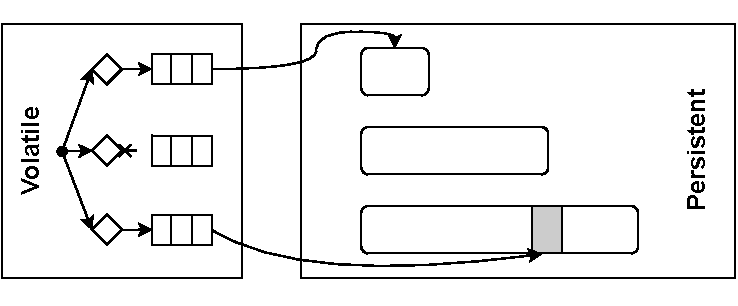
\includegraphics[width=\linewidth]{img/lsm_read}
    \caption{\acf{LSM-tree}. A read request first consults the
    bloom filters (in this case, the first yields a false
    positive, the second a true negative and the third a true
    positive) and subsequently performs a binary search on the
    fence pointers to find the block to get in each run, finding
    the target key (shaded) in the third
    run.}\label{fig:lsm_read}
\end{figure}

The key data structure for modern \acp{KVS} is the \acf{LSM-tree}.
Examples of industry-grade \acp{KVS} relying on \acp{LSM-tree} include
LevelDB~\cite{leveldb},
BigTable~\cite{bigtable}, Apache Cassandra~\cite{cassandra} and
RocksDB~\cite{rocksdb}. \acp{LSM-tree} have also been the topic of
a lot of recent research~\cite{lsm1,lsm2,lsm3,lsm4}.


The main objective of \acp{LSM-tree} is to improve the
scalability of both reads and writes of persistent \acp{KVS}. To
scale writes, the \ac{LSM-tree} creates an in-memory batch of
objects. Once it has filled up, it sorts the batch and sends it
to disk where it becomes a \emph{run}. To keep the data organized
for efficient reads, the \ac{LSM-tree} maintains similarly sized
runs on levels of exponentially increasing sorted runs. Once a
particular level becomes too full, it is sort-merged into a run
of the following level. To perform a read, a binary search is
performed on each run to find the object. To optimize IO costs,
two approaches are employed. First, arrays of fence pointers are
stored in memory, which allows us to perform the binary searches
in memory, reducing the IO cost per run to 1. Additionally, a
Bloom filter~\cite{bloom} can be constructed per run to filter
upfront which runs need not be checked. Figure~\ref{fig:lsm_read}
summarizes the architecture of an \ac{LSM-tree} responding to a
read request.


\begin{figure}[t]
    \begin{minipage}[t]{0.45\linewidth}
        \centering
        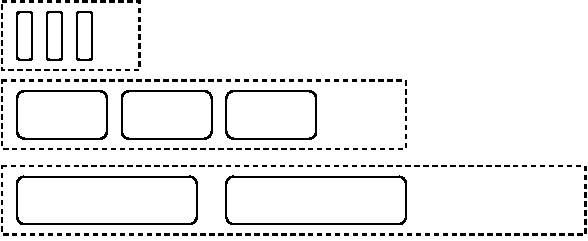
\includegraphics[width=\linewidth]{img/lsm_tiered}
        \caption{Tiered \ac{LSM-tree}.}\label{fig:lsm_tiered}
    \end{minipage}
    \begin{minipage}[t]{0.45\linewidth}
        \centering
        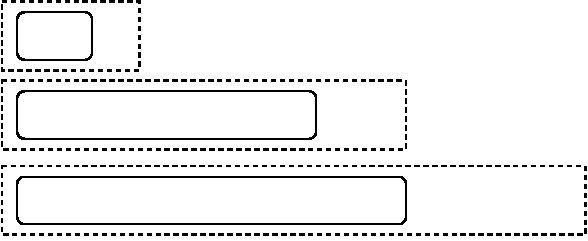
\includegraphics[width=\linewidth]{img/lsm_leveled}
        \caption{Leveled \ac{LSM-tree}.}\label{fig:lsm_leveled}
    \end{minipage}
    \caption{Comparison between a tiered and leveled
    \ac{LSM-tree}. The dashed boxes represent the capacity of the
    level and contiguous blocks denote sorted runs. In the tiered
    \ac{LSM-tree}, adding another run to the first level would
    trigger a sort-merge which would create another run at the
    second level. In the leveled \ac{LSM-tree}, each level is already sorted. }
\end{figure}

There are two classes of designs for \acp{LSM-tree}, levelling
and tiering \acp{LSM-tree}. In the tiereing approach, each level
gathers runs from the previous level, sorting them only when it
reaches capacity and pushing the newly-sorted run to the next
level. In the levelling approach, a run from the previous level
is merged as soon as it is received, ensuring the run is always
sorted. The tiering approach is tailored to write-intensive
workloads, since it does less work per object, while the
levelling approach is more read-optimized, as the runs are in a
sorted state, allowing for more efficient lookups.
Figures~\ref{fig:lsm_tiered} and~\ref{fig:lsm_leveled} show the
two different approaches.


\section{Persistence in replicated distributed systems}

The means by which persistence is achieved in replicated
systems is non-consensual within the distributed systems
community. Some authors consider that persistence requires
synchronizing the state of the replicas to a persistence
medium~\cite{gaios} (be it a magnetic disk, a solid state drive or non-volatile
memory) while others argue that persistence can be achieved by
replication~\cite{pbft,byz_fault_tolerant,hq,zyzzyva}. The latter approach, while avoiding expensive
accesses to persistent storage, makes it impossible to sustain a
full system shutdown. In practice, catastrophic failures
caused by natural disasters are generally unavoidable.
Moreover, forcing some replicas to be always up
makes it difficult to upgrade replicas simultaneously.

\paragraph{Persistence in distributed read-write registers}
Read-write register protocols have clear places where the state
needs to be persisted in storage: when a replica receives a write
(or writeback) request.  If the intended system is to be fully
in-memory, then this synchronization can be skipped. In general,
protocols for implementing these registers omit this
discussion~\cite{abd,time_efficient_abd}, leaving the decision
for system designers.

\paragraph{Persistence in replicated state machines}
Replicated state machines have been extensively studied from the
point of view of persistence and recovery. Although it is dubious
whether replicas are expected to synchronize to persistent state
in the original formulation of the Paxos algorithm~\cite{paxos},
the clarification paper~\cite{paxos-simple} published by Lamport
specifically requires replicas to synchronize to persistent
storage before replying.

Nevertheless, this has not prevented further research
from deviating from this prescription. PBFT~\cite{pbft}, which
implements replicated state machines in the Byzantine model,
considers that persistence is achieved through replication. Even
in the crash model, there have been attempts to either remove or
reduce the impact of persistent storage. Boichat \emph{et
al.}~\cite{winter} describe a recovery protocol for Paxos, which
they call \emph{Winter}, where persistent storage is never used.
However, this is done by assuming that a strict majority of nodes
is always up, which severely limits the practicality of the
solution.

A more recent attempt~\cite{recovery-paxos} to improve on recovery protocols for
replicated state machines using Paxos proposed two protocols
which only write to disk infrequently (either on leader changes
or in the case of a restart). They achieve this by assuming that
a majority of nodes is never simultaneously faulty. This
assumption, albeit stricter than the one made by \emph{Winter},
still makes it impossible to sustain a full system
shutdown.

\cleardoublepage{}

\fancychapter{The \ac{RR} Fault Model and Its Protocols}\label{chap:model}
\cleardoublepage{}

In this chapter, we define the \ac{RR} fault model, which
captures the behaviour of replicated nodes with persistent state.

We will motivate this fault model from its origins as a fault model
for replicated \acp{TEE} with persistent state, and subsequentely
we will motivate how this fault model can further be applied to
nodes with persistent storage replicated using the crash fault
model. Then, we derive requirements for quorum systems in the
\ac{RR} model, as well as their intersection properties, a key element to the
correctness of replication protocols.

Building on the quorum system abstraction, we explain how to
adapt existing \ac{CFT} protocols to the \ac{RR} model. We
provide two concrete examples of such adaptations using
well-established protocols: the \ac{ABD}~\cite{abd} protocol for
a read-write register and the Paxos~\cite{paxos} protocol for
\ac{SMR}. We conclude this chapter with a discussion.

We then provide a performance evaluation in the context of
\acp{TEE} using micro-benchmarks. We compare the \ac{CFT}
protocols with their adaptations to the \ac{RR} model and the
equivalent counterparts in the \ac{BFT} world. This demonstrates
the viability and usefullness of the \ac{RR} model in the context
of \ac{TEE}-based replication, showcasing how it enables
protocols with both correctness (otherwise only found in
\ac{BFT}) and speed (present in \ac{CFT}-based replication).

\section{Motivation}\label{sec:motivation}

\subsection{\ac{TEE} properties}\label{ssec:tee_motivation}

In this section, we review the properties of \acp{TEE} and motivate the
\ac{RR} fault model. While the precise guarantees provided by a
\ac{TEE} vary with the \ac{TEE} design, we can summarize common guarantees across platforms.

\paragraph{Confidentiality.} \acp{TEE} allow a computation to execute with
hardware-enforced confidentiality over the internal code and data used
by the computation. Data and instructions are decrypted in hardware as
they are fetched from memory inside the CPU chip and modified data is
re-encrypted before it leaves the CPU chip. Only code executing inside
the \ac{TEE} has access to cleartext data, therefore ensuring
confidentiality even from \ac{OS}, hypervisor, and platform
operators.

\paragraph{Integrity and attestation.}
%\acp{TEE} also protect the integrity of computations.
When a \ac{TEE} is started, the secure platform computes a hash of the
\ac{TEE}'s initial code and data and compares it to the expected {\em
  measurement} hash for the instance. Only when this {\em attestation}
succeeds is the \ac{TEE} provided with the key material it needs to
authenticate itself to third parties and to access and decrypt
persistent data stored externally on its behalf.  A remote party can
ascertain that it is communicating with a \ac{TEE} instance that has a
particular initial measurement hash and executes on a legitimate \ac{TEE}
platform via {\em remote attestation}.  Furthermore, to protect the
\ac{TEE}'s integrity during execution, the hardware isolates the \ac{TEE} and
detects modifications of encrypted code and data while stored in main
memory. Some implementations like Intel SGX even protect code and data
from certain physical attacks. % using a bus probe.

\paragraph{State continuity in the presence of external state.}
\acp{TEE} can stored encrypted state in external persistent storage across
activations through a process called {\em sealing}.  As described
above, a correctly attested \ac{TEE} receives a secret key unique to its
instance, which allows the \ac{TEE} to store encrypted external state with
confidentiality and integrity guarantees.  To ensure the {\em recency}
of its external state, however, a \ac{TEE} must ensure that the encrypted
external state it is presented with after a restart is the most recent
version it had previously stored. More generally, \ac{TEE} computations may
require the strictly stronger property of {\em state continuity},
which requires that a \ac{TEE} never executes an operation with a stale
state, or executes different inputs from the same
state~\cite{ariadne}.

\ac{TEE} implementations lack general, high-performance support to ensure
freshness and state continuity for computations with external state.
Some \ac{TEE} platforms provide trusted, persistent monotonic counters
associated with the CPU platform. While these counters are sufficient
in principle to ensure state continuity, they are not sufficient in
practice~\cite{ariadne}.  In particular, hardware intentionally slows
the time to increment these counters to milliseconds in order to avoid
wrap-around attacks~\cite{ariadne,rote}.  As a result, such counters
can at best support state continuity for \acp{TEE} that exhibit infrequent,
orderly shutdowns, during which a \ac{TEE} can update the counter and store
its external state with the latest counter value
embedded~\cite{ariadne}.  However, trusted counters are inadequate for
\acp{TEE} that frequently update their external state (e.g., a database or
\ac{KVS}) and can crash at any time; ensuring state continuity
for such \acp{TEE} requires rapid counter updates.  Moreover, trusted
counters are tied to a particular CPU/motherboard and do not support
safe migration of \ac{TEE} computations.

Note that state continuity implies fork
protection~\cite{fork_lcm}, i.e., guaranteeing that no duplicate
\ac{TEE} are instantiated with access to the same stored state.
We discussed how fork protection and how it can be achieved in
replicated systems in Chapter~\ref{chap:related}.

\paragraph{\ac{TEE} threat model and guarantees.}

The design of \acp{TEE} assumes a powerful adversary, who has full
control over the operating system and hypervisor that hosts a \ac{TEE}.
The adversary can arbitrarily create and shutdown \ac{TEE} instances at
any time, as well as delay, read, drop or modify all messages sent
to and received by enclaves.  Moreover, an adversary can tamper with
or replace the external (encrytped) state associated with a \ac{TEE}
instance.

\ac{TEE} security is rooted in the hardware design and implementation, as
well as the vendor's certificate chain used for remote attestation. As
a result, the threat model of \acp{TEE} excludes compromise of the vendor's
\ac{TEE} platform design and implementation, physical attacks on the CPU
chip, or compromise of the vendor's certificate chain.  Some \ac{TEE}
implementations also exclude physical attacks using bus probes.  Side
channels are outside the threat model of current \acp{TEE}.

\paragraph{Choosing a fault model for replicated \acp{TEE}}

Subject to the \ac{TEE} threat model, computations that do not depend on
external state enjoy confidentiality and integrity, and can be
considered to suffer only crash faults (as opposed to Byzantine
faults, where an adversary may induce arbitrary behavior in a
component). Therefore, a crash-tolerant replication protocol is sufficient
to replicate \ac{TEE}-encapsulated computations that don't use external
state.  If a \ac{TEE} computation relies on external state, however, then
it can additionally suffer a rollback of the external state to an
earlier version whenever the \ac{TEE} restarts.  This behavior is beyond
the crash fault model; therefore the use of crash-tolerant replication
protocols is not safe. Currently, \ac{BFT} protocols are typically used
instead~\cite{teechain,rote}.  Using \ac{BFT} is safe but needlessly
expensive, because these protocols are designed to tolerate arbitrary
behavior, most of which is masked by the properties of \acp{TEE}.
In the Section~\ref{sec:model}, we describe a novel fault model that
captures {\em precisely}\ the set of behaviors exhibited by \acp{TEE} with
external state: crash failures plus state rollback after a restart.

\new{
\subsection{Extending the usefulness of fault model}\label{sec:extending_fault_model}

Although the \ac{TEE} use-case requires something like the
\ac{RR} model out of \emph{necessity}, we also look at \ac{RR} as
an \emph{oportunity}. The ability to tolerate some rollbacks on
restart is useful outside the security sensitive context of
\acp{TEE}. Consider a replicated \ac{KVS}, where each node
maintains a local \ac{KVS}. When writing to the local key
value store, there are three possible approaches:
\begin{enumerate}
    \item[A.] The node synchronizes the written object
        immediately, and then replies. This impacts
        \emph{throughput};
    \item[B.] The node places the object in a batch, and waits
        for the batch to be flushed before replying. This impacts
        \emph{latency};
    \item[C.] The node places the object in a batch, and
        immediately issues the reply. This offers the best
        throughput and latency, but can lead to \emph{data loss}
        if the replica crashes (i.e.: if it suffers a rollback);
\end{enumerate}

\ac{RR} opens the possibility of a hybrid approach, where some
nodes place the object in the batch and reply eagerly (approach
C), while others bypass the batch and synchronize directly to
disk (approach A). With careful orchestration, this can in principle allow for
a throughput advantage compared to approach A, a latency
advantage compared to approach B and a durability advantage
compared to approach C, a very interesting tradeoff.
}

\section{\ac{RR} model definition}\label{sec:model}

Nodes in the \ac{RR} model are network-connected processes with external
persistent state. Nodes can crash at any point in their execution
and restart at a later instant.  Additionally, nodes can suffer a
rollback failure upon a restart, after which their externally
stored, persistent state may be valid but stale.  After each
restart, nodes flag their state as suspicious when replying to
requests, signalling that they have restarted and thus may have
been subject to a rollback. Nodes can reliably determine when it has executed its
initialization code and thus restarted. A node stops indicating
the suspicious flag once it is ascertained that its state is
fresh, e.g., by ensuring that a sufficiently large number of
other nodes have the same state (as we exemplify in
Section~\ref{sec:protocol}).

Nodes execute the algorithm correctly, with this exception
concerning state freshness. Figure~\ref{fig:states} illustrates
the state transitions a node in the \ac{RR} model can go through.

\begin{figure}[t]
    \centering
    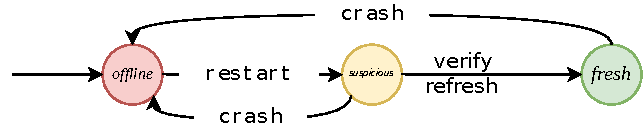
\includegraphics[width=\linewidth]{img/RR_states}
    \caption{States of a node in the \ac{RR} model. Compared
      to the crash-fault model, there is an additional ``Suspicious''
      state.}\label{fig:states}
\end{figure}

\subsection{Replicated systems}\label{ssec:sys_model}

Replication protocols make a separation between clients machines
and replicas, where these two groups of nodes are connected by a
network through which any pair of nodes may communicate, defining
what is referred to as a message-passage system. These replicas
collectively implement a replicated service exporting a set of
operations, which clients may invoke. For instance, a storage
system may export a simple interface with read and write
operations, whereas a replicated database has a richer interface
supporting SQL operations. To collectively implement a replicated
service, replicas store their view of the current state of the
system that is shared among multiple clients, and client
operations are implemented by contacting a group of replicas to
either query or update that state. In general, replication
protocols leverage a ``quorum RPC'' communication
pattern~\cite{Malkhi:Reiter:BQS:98,lorenzo:framework} where a
machine (either a client or one of the replicas) sends a message
to a group of replicas and waits for a reply from a quorum. In
the fault tolerance literature, a quorum is a set of subsets of
the group of replicas, where these subsets have certain
intersection properties that are important for the protocol
correctness~\cite{gifford:quorums}. These intersection properties
depend on the fault model, e.g., with crash faults it normally
suffices that any two quorums have a non-empty
intersection~---~majorities are an example of a quorum system
with this property. Byzantine quorums, in turn, require a larger
intersection to account for incorrect replies from malicious
replicas~\cite{Malkhi:Reiter:BQS:98}.

\subsection{Replication in the \ac{RR} model}

A key insight of replication in the \ac{RR} model is to grow quorums
\emph{dynamically} when replicas are suspicious of their state.
We quantify this suspicion by counting, in each instance of the
quorum RPC pattern, how many replicas indicated the suspicious
flag, and we refer to this count as a per-RPC variable $s$.
In addition to this (dynamic) value, we also define a (static)
maximum bound on the number of nodes that may actually
suffer a rollback attack within the replica group, $M_R$.

Note that $s$ and $M_R$ are different and unrelated in several
respects. First, $s$ is measured by a node that gathers a set of
replies, and therefore its value is specific to each invocation
of an operation on a group of replicas, whereas $M_R$ is a
constant bound that is assumed to hold for that group of replicas
during the entire execution of the system. As a consequence, $s$
cannot be set at system configuration time, whereas $M_R$ needs
to be set by an administrator according to an expectation of the
deployment conditions. Second, $s$ can vary from zero (common
case, no recent replica restart) up to $N$ (simultaneous system
shutdown followed by a restart). In contrast, $M_R$ will be
parameterized according to the likelihood of a correlated
rollback attack, which in turn depends on the deployment and its
independence expectations. For example, one could deploy replicas
across different administrative domains, in which case (and
assuming that there is no collusion between administrators of
different domains), $M_R$ should be at least the maximum number
of replicas within a single domain. This encompasses the worst
non-colluding attack where a malicious administrator rolls back
all the replicas in the domain simultaneously.

Note that the parameter $M_R$ also subsumes permanent crash
faults (e.g., due to permanent hardware failure), since permanent
crashes can be seen as a particular instance of a rollback, where
we replace a failed node with a new one that starts from the
initial state of the system (or fetches a recent but possibly not
the most recent one).
%
Finally, we define a liveness bound $F$, i.e. the system is live
provided that no more than $F$ replicas are temporarily unreachable at
any given moment, due to network partitions, power outages, or reboot.

\subsection{Deriving {\ac{RR} Quorums}}\label{ssec:parameters}

As we explained, the correctness of replication protocols hinges
on the property of quorum intersection: any pair of operations
executed in the system must execute in replica subsets (or
quorums) that intersect sufficiently for the system to return a
result that obeys the protocol specification. We now revisit this
intersection property for the design of protocols for the \ac{RR}
model. To this end, we need to first specify the set of
properties that this intersection should achieve.


\begin{property}[Freshness]
    The safety property of replicated systems normally includes
    the need for the most recently written value to be seen by
    subsequent operations. In quorum-based protocols, this
    property is enforced by ensuring that any pair of quorums
    intersects in at least one replica that does not deviate from
    its prescribed behavior. In the case of the \ac{RR} model, a
    correct replica is one that has received the most recent
    write and has not been rolled back.
\end{property}


\begin{property}[Durability]
    Durability is guaranteed if any operation that updates the
    state of the system survives any combination of faults that
    is allowed by the \ac{RR} model. In our case, this means that
    even if $M_R$ replicas are rolled back, there will be at
    least one replica with the up-to-date value.
\end{property}

\begin{property}[Operational Liveness]
    Generally, a system is live if all operations it supports eventually
    conclude.  We consider a more granular property of operational
    liveness, which separates the liveness with respect to two classes
    of operations that are normally defined in replicated systems:
    read-only (or simply read) operations, which query but do not modify
    the replicated state, and update (or write) operations that may
    operate on that state to create a new system state or simply overwrite
    it.
\end{property}

Using these properties, we place constraints on the composition
of the quorum systems. We differentiate read quorums, of size
$R_Q$, which are sufficient to conduct read operations, from
write quorums, of size $W_Q$, for write operations.

\paragraph{Freshness.}

We start by observing that, for a given read operation and within
the entire replica set, the number of nodes that could possibly
have their state rolled back is $\min(s, M_R)$. This means that a
read operation has access to a pool of replicas where $W_Q -
\min(s, M_R)$ are up-to-date and $N - W_Q + \min(s, M_R)$ may be
stale. Given that the most recent write operation contacted $W_Q$
nodes, thus bringing them up-to-date, we derive the following
minimum size for a read quorum:
\begin{equation} \label{eq:inters}
  R_Q > N - W_Q + \min(s, M_R)
\end{equation}

In our derivation, we turn the inequalities into equalities by
adding a positive (or in some cases non-negative) $\Delta$
parameter, which captures by how much each variable is larger
than strictly necessary, in this case:
\begin{align} \label{eq:inters2}
  R_Q = N - W_Q + \min(s, M_R) + \Delta_R && \Delta_R > 0
\end{align}

\paragraph{Durability.}

Additionally, we note that, since $M_R$ replicas can be rolled
back, surviving such a rollback implies that a write quorum must
include more than $M_R$ replicas, i.e.,
\begin{align}
    W_Q &> M_R \nonumber \\
    W_Q &= M_R + \Delta_W && \Delta_W > 0 \label{eq:fresh}
\end{align}

\paragraph{Write Liveness.}
We must also guarantee liveness for write operations. This
requires that a write quorum is available despite $F$ unreachable
nodes. This is guaranteed provided that:
\begin{align}
    N - F &\geq W_Q \nonumber \\
    N &= W_Q + F + \Delta_N && \Delta_N \geq 0  \label{eq:Wavail}
\end{align}


\paragraph{Final Derivation.}
The formulae above allow us to arrive at a precise formulation
for the system and quorum sizes. In particular, by
combining~\ref{eq:fresh} and~\ref{eq:Wavail}, we obtain:

\begin{align} \label{eq:ReplSize}
  N = M_R + F + \Delta_W + \Delta_N && \Delta_W > 0, \Delta_N \geq 0
\end{align}

Then, by replacing $W_Q$ (\ref{eq:fresh}) and $N$
(\ref{eq:ReplSize}) in Equation~\ref{eq:inters}, we obtain the
following equation for read quorums.
\begin{align}\label{eq:ReadSize}
  R_Q = F + \min(s, M_R) + \Delta_N + \Delta_R && \Delta_R > 0, \Delta_N \geq 0
\end{align}

\paragraph{Read Liveness.}
We conduct the analysis of the liveness conditions for read
quorums separately, since these are dynamic conditions, namely
due to their dependency on the current number of possibly stale
nodes, $s$.  As such, we introduce another dynamic value: $f^{\prime}$,
the number of replicas that are unreachable at any given point.
This allows us to express the dynamic liveness condition for
reads as follows:
\begin{equation}\label{eq:DynRavail}
    N - f^{\prime} \geq R_Q  \Leftrightarrow f' + \min(s, M_R) \leq M_R + \Delta_W - \Delta_R
\end{equation}

This equation allows us to reason about the liveness for reads,
depending on specific runtime conditions and on how the static
parameters are chosen. For instance, we could require reads to be
live in the worst possible case of $f^{\prime} = F$ and $s = M_R$, yielding
$\Delta_W \geq \Delta_R + F$.

However, this is a conservative assumption. An example of a more
realistic one would be to assume that we forfeit read liveness in
the event of a worst case level of unreachability ($f^{\prime} = F$) and
there is at least one rollback ($M_R \geq 1$). This yields
$\Delta_W \geq \Delta_R + F - r$. We also choose to set
$\Delta_N=0,\Delta_R=1$ to minimize replication costs, allowing
us to derive the value for $\Delta_W$ from
Equation~\ref{eq:DynRavail}:
\begin{align} \label{eq:deployment1}
  \Delta_W &\geq  \Delta_R + F - M_R\\
  \Delta_W &\geq  1 + F - M_R
\end{align}

When also taking into account that $\Delta_W > 0$, and turning
the inequality into an equality to minimize replication costs,
this allows us to derive:
\begin{align} \label{eq:deployment2}
  \Delta_W &=  \max(1,1 + F - M_R)\\
  \Delta_W &=  1 + \max(F - M_R,0)
\end{align}

This results in these possible deployment parameters:
\begin{align} \label{eq:deploymentfinal}
    N &= \max(M_R, F) + F + 1  \\
    W_Q &= \max(M_R, F) + 1 \\
    R_Q &= F + \min(s, M_R) + 1 \label{eq:proof3}
\end{align}

\paragraph{Atomic update operations.}
As we mentioned, more complex systems such as replicated
databases, instead of following a simple read/write interface,
support rich operations that read the most recent value of the
system \emph{and} update it with a new value derived from the
value that was read. To achieve this, their protocols may need to
gather both a read and a write quorum (i.e., $\max(R_Q, W_Q)$
replies). We dub these quorums \emph{super quorums} and use $S_Q$
to represent their size.

\paragraph{Quorum properties.} This derivation of the various quorum
sizes leads to the following set of properties that \ac{RR} quorum
systems obey (also illustrated in Figure~\ref{fig:quorums}):

\begin{enumerate}
    \item[\textbf{I1.}] Any read quorum intersects with any write
        quorum in at least one replica whose state was not rolled
        back;
    \item[\textbf{I2.}] It is possible some pairs of read quorums
        do not intersect.
\end{enumerate}

Using these properties, we can derive the following
property of super quorums:

\begin{enumerate}
    \item[\textbf{I3.}] The intersection between a super quorum
        and a quorum of any other type is non-empty and includes
        a replica whose state has not been rolled back.
\end{enumerate}

These properties, along with the fact that read quorums can be
smaller than write quorums in the normal case when there
are no restarts, play a role in the design and performance of
protocols in the \ac{RR} model, as we will see next.

\begin{figure}[t]
    \centering
        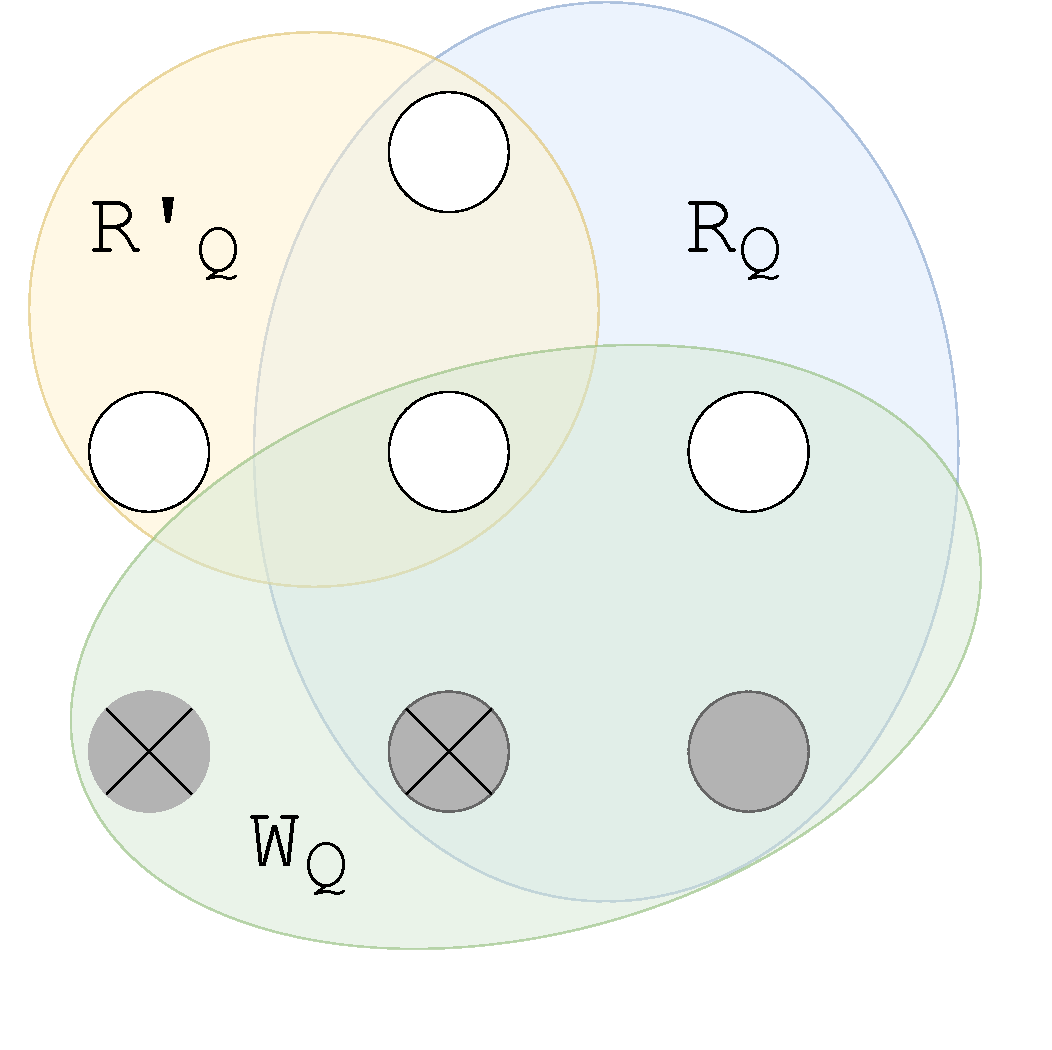
\includegraphics[width=.32\linewidth]{img/RR_quorums_I1}
        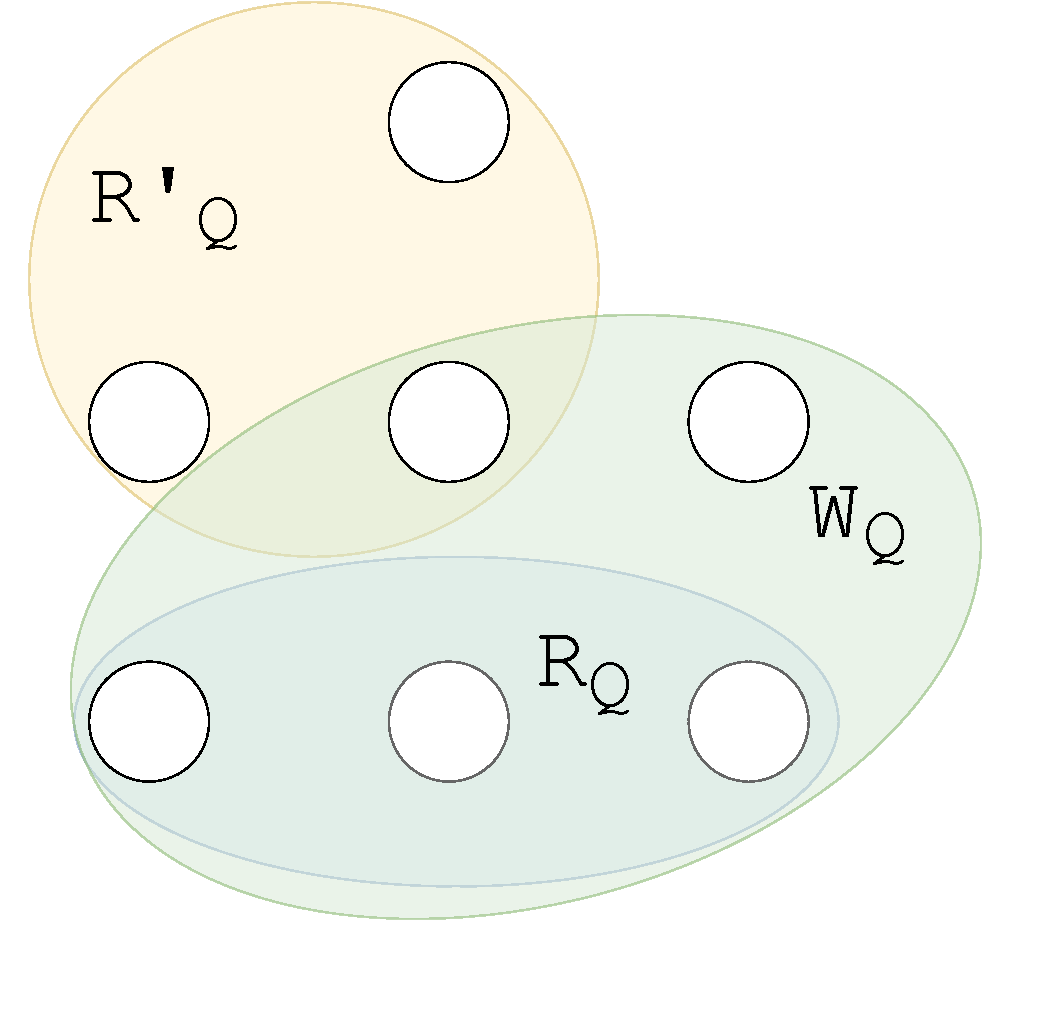
\includegraphics[width=.32\linewidth]{img/RR_quorums_I2}\\
        (a) \hspace{2.3cm} (b) \hspace{.2cm}
    \caption{Example of a partially intersecting \ac{RR} quorum system ($M_R=4$,
    $F=2$). In (a), there were $3$ restarts (shaded) and $2$ rollbacks
    (crossed). Thus, the read quorum receives suspicious replies and
    grows larger, ensuring that both read quorums still intersect $W_Q$ in
    at least one up-to-date replica (as required by \textbf{I1}).
    In (b), there are no restarts (and, by extension, no
    suspicion of rolled back state), and thus read quorums can be
    disjoint, as noted by \textbf{I2}.}\label{fig:quorums}
\end{figure}

\paragraph{Classifying \ac{RR} Quorum Systems}
Reviewing the quorum properties in the previous paragraph,
there is one property that stands out: \textbf{I2}. In quorum
literature, the intersection of quorums is a key property, but
in \ac{RR}, it naturally arises that, for some
parametrizations, this is not guaranteed to happen between all
read quorums. Here, two disjoint read quorums may in general
reflect different system states~---~a phenomenon usually
described as {\em split brain}.  This can happen when an
operation that changes the system state is still in progress (or
even halted, due to the crash of the initiator). Handling this
peculiarity will require some protocol support, creating
mechanisms to ensure that a single value is reported by all read
quorums. However, in certain parametrizations, property
\textbf{I2} can be guaranteed never to hold, and thus such
extraneous protocol infrastructure can be avoided. We classify
\ac{RR} quorum systems in two categories accordingly:

\begin{defin} [Partially Intersecting \ac{RR} Quorum System]
    A \ac{RR} Quorum System in which there are two read
    quorums, $R_Q^1, R_Q^2$ such that $R_Q^1 \cap R_Q^2 =
    \O$. In other words, where \textbf{I2} holds.
\end{defin}

\begin{defin} [Fully Intersecting \ac{RR} Quorum System]
    A \ac{RR} Quorum System in which for all pairs of read
    quorums, $R_Q^1, R_Q^2$ $R_Q^1 \cap R_Q^2 \neq
    \O$ is true. In other words, where \textbf{I2} does not
    hold.
\end{defin}

Theorem~\ref{theorem:fully_intersecting} describes how to
characterize a \ac{RR} quorum system as either partially or
fully intersecting based on its parametrization:

\begin{theorem} [Characterization of \ac{RR} Quorum
    Systems]\label{theorem:fully_intersecting}
    A \ac{RR} quorum system with parameters $M_R, F,
    \Delta_R, \Delta_W$ and $\Delta_N$, where $\Delta_R > 0,
    \Delta_W > 0$ and $\Delta_N \geq 0$ and in which the
    total number of replicas is $N = M_R + F + \Delta_W +
    \Delta_N$, the size of read quorums is $R_Q = F + \min(s,
    M_R) + \Delta_N + \Delta_R$ (with $s$ as defined above)
    and the size of write quorums $W_Q = M_R + \Delta_W$ is
    fully intersecting if and only if:
    \begin{equation}\label{eq:charaterization_theorem}
        F + \Delta_N + 2 \Delta_R > M_R + \Delta_W
    \end{equation}
\end{theorem}
\begin{dem}
    To prove the intersection of any two read quorums, it
    suffices to show that
    Equation~\ref{eq:charaterization_theorem} is equivalent to $2
    R_Q > N$, even when $s = 0$. This in turn is equivalent to
    stating that the dimension of \emph{any} two read quorums
    from the set of the smallest read quorums possible for a
    quorum system (i.e.: those where $s = 0$) is larger than the
    size of the quorum system. This implies that at least one
    replica is present in both read quorums, and as such property
    \textbf{I2} cannot hold. We denote the size of the smallest
    read quorums as $R_Q(s = 0)$.
    \begin{align*}
        2 R_Q (s = 0) &> N  \\
        \equ 2F + 2\min(0, M_R) + 2\Delta_N + 2\Delta_R &> M_R + F + \Delta_W + \Delta_N  \\
        \equ F + \Delta_N + 2\Delta_R &> M_R + \Delta_W \\
    \end{align*}
    \hfill\ensuremath{\Box}\vspace{2em}
\end{dem}

\begin{corollary}
    In the parametrization in
    Equation~\ref{eq:deploymentfinal}, the associated quorum
    system is fully intersecting if and only if $F \geq M_R$
\end{corollary}
\begin{dem}
    The parametrization in question fixes $\Delta_R = 1,
    \Delta_W = 1$ and $\Delta_N = 0$. Substituting in
    Equation~\ref{eq:charaterization_theorem}, we get:
    \begin{align*}
        F + 2 &> M_R + 1 \\
        \equ F + 1 &> M_R \\
        \equ F &\geq M_R
    \end{align*}
    \hfill\ensuremath{\Box}\vspace{2em}
\end{dem}
}

\paragraph{Reflections on the parametrization of the system.}
\ac{RR} quorums are more complex than regular
quorum systems. They include two parameters ($M_R$ and $F$) instead of
one, with an additional runtime value ($s$). Moreover, the quorum
system is inherently asymmetric, leading to three different types of
quorums (read, write, and superquorums), as opposed to a single one.
This puts a burden on the system designer to use the right type of quorums for
different protocol steps, and also, at deployment time, to consider how to
choose $M_R$ (to represent the anticipated maximum number of simultaneous rollback
attacks on the system), and $F$
(to encode the availability of the system, by estimating how many replicas
can crash without jeopardizing liveness).
%
However, we believe that this complexity is warranted, not only
because it is naturally derived from the nature of the faults (in
particular, the fact that it is possible to determine precisely when a
replica is or is not susceptible to a rollback of its persistent
state), but also because it allows us to extract the maximum
performance from the system and avoid wasting resources used in
replication.

\paragraph{Comparison with existing asymmetric quorum schemes.}

Previous proposals for asymmetric quorum schemes differ
significantly from \ac{RR} quorum systems.  The idea of
asymmetric quorums dates back to one of the initial proposals for
quorum systems by Gifford~\cite{weighted_voting}, where a
replicated object has a certain number of votes and in order to
read the value, $r$ votes must be gathered, whilst $w$ votes
are required to write the value. The equivalent to the
intersection property \textbf{I1} is guaranteed by ensuring that
$r + w$ exceeds the total number of votes of the object. This use
of asymmetric quorums has also been motivated by different goals.
In particular, asymmetric quorums have been proposed in the
context of asymmetric trust assumptions~\cite{asymmetric_trust},
where each node makes its own assumptions about which nodes might
be Byzantine. Another type of use of asymmetric quorums is to
obtain better performance, by making the commonly used quorums
smaller than the ones that are used less
often~\cite{fp,wheat,rqs} or reducing the asymptotic complexity
of quorums at the expense of more replicas~\cite{grid_quorums}.

Compared to these approaches, \ac{RR} quorums are derived from
the dynamic nature of the number of possible rollbacks that are
present in the system at any given moment. This natural
construction leads to interesting properties of the system,
namely allowing for performance to improve in the normal case
when there are no recent replica restarts, due to the use of
relatively small read quorums.

\section{Replication protocols}\label{sec:protocol}

Designing and implementing new replication protocols, as well as
proving their correctness, is a non-trivial effort. Consequently,
rather than building protocols for the \ac{RR} model from
scratch, we propose a set of principles for adapting existing
protocols to the fault model. In this section, we identify
principles for this adaptation and apply them to existing
protocols, showing that the adaptation is straightforward.

\subsection{Principles and challenges for protocol adaptation}\label{ssec:adaptation}

When adapting existing protocols to the \ac{RR} model, it is
convenient to start from a crash fault tolerant protocol.
Due to the correctness of execution of nodes in the \ac{RR}
model, nodes observe mostly crash fault behavior; the only
additional fault behavior is that their externally stored state
may be stale after a restart.

Most replication protocols are quorum-based, where a client (or a
replica acting on behalf of a client) needs to obtain responses
from the quorum or replicas to perform an operation.  Therefore,
an important aspect of adapting a crash fault tolerant protocol
consists of following the quorum sizes defined in
Section~\ref{ssec:parameters}. Similarly, reconfiguration is a
key aspect of practical replication protocols. Quorum sizes for
these reconfiguration protocols also need to be adapted
accordingly\new{, either to be a write quorum or a super quorum,
depending on whether the update needs to be atomic}.

Each node must be augmented to maintain a suspicion flag. When a node
restarts, it set the suspicion flag to true. At this point, the node
runs a recovery subprotocol (eagerly or lazily), which is not required
in the crash model.

While the recovery subprotocol is dependent on the specifics of
the protocol being modified, the general method is as follows. On
restart, a replica queries a read quorum of replicas for a digest
of their state, retaining the replies that contain the most
recent state, e.g., determined through timestamps as exemplified
next.  From this read quorum of digests, it can determine the
digest of the current system state, and check whether its state
is up-to-date, thus clearing the suspicion flag. If not, then the
specific parts of the state that are stale need to be fetched
from other replicas to bring the recovering replica up-to-date.
To efficiently find which elements of the state are out of date,
replicas may maintain a Merkle tree, which allows for determining
which parts of the state need to be fetched without transmitting
a large amount of information. Note that this subprotocol can run
lazily and in the background, while the replica continues
satisfying requests\rr{replying to them only in case the state is
guaranteed fresh}\bsd{no, always replies, but sets the suspicion
flag}. Doing so might allow for clearing the
suspicion flag in case of an update where the new state does not
depend on the previous version.

If the quorum system is \emph{fully intersecting}, these changes
are enough. Otherwise, mechanisms that ensure the correctness of
reads from possibly disjoint read quorums need to be put in
place. These mechanisms will be generally protocol specific.

\bsd{point forward about preemptive and cautious
approaches?}\rr{huh?}

Next, we will present two example protocols that follow these
principles and illustrate some of the above challenges.

\subsection{Read-write register}\label{ssec:abd}

In this section, we present an adapted version of the
ABD~\cite{abd} protocol for a distributed read/write register
with linearizable semantics\footnote{A concurrent object is
linearizable iff there exists a serialization of all operations
which is equivalent to a sequential execution and the
serialization matches the real-time order of
invocation/reply.}~\cite{linearizability} under the \ac{RR}
model. ABD provides a simple read/write interface, which is
useful for storage systems or services that offer a read/write
interface. Read/write register protocols have the advantage of
guaranteeing termination even in asynchronous systems with
faults, and having good performance due to a simple message
pattern that is linear in the number of
replicas~\cite{gryff:nsdi20}.
%
Figure~\ref{fig:abd-read} shows the pseudocode for the read
operation, while the write logic is shown in
Figure~\ref{fig:abd-write}. Since the code follows closely the
original ABD protocol, our explanation highlights where we
adapted the protocol to the new fault model.

\paragraph{Timestamp Structure.}
Each data item stored is associated with a
timestamp, which defines the linearization order of the version
that is stored. Timestamps have two numeric components $\langle
seqno, client\_id \rangle$, where $client\_id$ is the
unique, ordered id of the client issuing the write.  This
breaks ties when two clients write different values to the same
sequence number.
%Additionally, there is a $stable$
%boolean flag, associated with the timestamp, indicating whether
%the vallue is stable or not.

\paragraph{Write.}  This operation is similar to the ABD
protocol, but uses the \ac{RR} quorum system. In the first round
a read quorum is gathered to discover the most recent sequence number
(the one associated with the highest timestamp).  In the second round,
that sequence number is incremented by the client, appended with the
client id, and the resulting timestamp is sent with the value to be
written. Upon receiving this second round message, replicas overwrite
values if the received timestamp is greater than the one associated
with the data they store. This clears the suspicion that may have
existed of the value of the register, as the written value is
guaranteed to be fresh.


\paragraph{Read.} Following the ABD protocol, reads occur in one
round in the common case, with a second round being required if a
value needs to be written back. In particular, in the original ABD
protocol, the first round queries replicas for their data and
timestamp, waits for replies from a majority (which equates to both a
read and a write quorum) and the return value corresponds to the reply
with the highest timestamp. However, when there is no majority that
holds that timestamp value, the second phase is required, writing this
timestamp and data to a majority. (This is needed to conclude a write
operation that executes concurrently or was left unfinished.)

Translating the notion of a majority to read and write quorums in the
\ac{RR} model presents a subtle challenge in the context of
partially intersecting quorum systems. Even though
intuitively the initial read round only requires a read quorum (and in
fact this is sufficient to determine the read reply), the optimization
of skipping the second round is only applicable if there is unanimity
for that timestamp in a write quorum. This is because read quorums do
not necessarily intersect (property \textbf{I2}), which implies that
contacting only a read quorum would allow for a ``split brain''
situation, where clients read different values depending on which
quorum they contact, thus breaking linearizability. The problem with
waiting instead for a super quorum, however, is that in scenarios
where inter-node latency has a wide variance such as geo-replication,
this introduces an additional latency that erodes the performance
advantage of the smaller quorums.

%We address this through a stabilization phase described next, which is useful beyond the use of this fault model, namely to asymmetric non-intersecting quorums in crash fault tolerant protocols.

%% Although having an ultimately protocol-dependant solutions, the
%% approach is common. The split-brain situation described above is
%% always a result of an in-progress write, meaning we need to
%% identify when this situation is actually occuring and employ
%% mechanisms to make sure that only one of the disjoint
%% read-quorums can return a value (and the other read operations
%% would need to fall back on larger quorums).

\begin{figure}[t]
  \begin{small}
    \textbf{Read} at client $c$

    \begin{enumerate}[itemsep=0pt,parsep=0pt]

    \item \textbf{send} $\textsc{read-replica}$ to all replicas

    \item \textbf{wait until} received  \textbf{either} $R_Q$ replies, such that, for the highest timestamp $ht$, $ht.stable==\textsc{true}$
       \textbf{or until} received $W_Q$ replies where the highest timestamp has $ht.stable==\textsc{false}$

    \item \textbf{if} $ht.stable==\texttt{true}$ \textbf{then}\\
        \tabto{.5cm}   \textbf{return} $\textsc{success}(ht,val(ht))$

    \item \textbf{if} $\exists W_Q$ of replies with $ht$ \textbf{then}\\
        \tabto{.5cm} \textbf{send} $\textsc{stabilize}(ht)$ to all replicas;\\
        \tabto{.5cm} \textbf{return} $\textsc{success}(ht,val(ht))$
    \item \textbf{send} $\textsc{write-replica}(ht,val(ht))$ to all replicas
    \item \textbf{wait until} received $W_Q$ of \textsc{success} replies

    \item \textbf{send} $\textsc{stabilize}(ht)$ to all replicas
    \item \textbf{return} $\textsc{success}(ht,val(ht))$

    \end{enumerate}

  \end{small}
  \caption{Pseudo-code for the register read operation.}\label{fig:abd-read}
\end{figure}

\begin{figure}[t]
  \begin{small}
    \textbf{Write (value $v$)} at client $c$

    \begin{enumerate}[itemsep=0pt,parsep=0pt]

    \item \textbf{send} $\textsc{read-replica}$ to all replicas

    \item \textbf{wait until} received $R_Q$ replies

    \item \textbf{let} $ht$ be the largest timestamp in quorum

    \item \textbf{let} $new\_ts$ be $\langle ht.seqno + 1, c, \texttt{false}\rangle$

    \item \textbf{send} $\textsc{write-replica}(new\_ts,v)$ to all replicas

    \item \textbf{wait until} received $W_Q$ \textsc{success} replies

    \item \textbf{send} $\textsc{stabilize}(ht)$ to all replicas
    \item \textbf{return} $\textsc{success}$
    \end{enumerate}

  \end{small}
  \caption{Pseudo-code for the register write operation.}\label{fig:abd-write}
\end{figure}

\paragraph{Stabilization.}
To address this issue, we introduce an extra asynchronous phase,
called the \emph{stabilization} phase. This phase takes
place in the background after a value has been successfully
written to a write quorum (either in a write operation or in the
writeback phase of a read operation), without
blocking the operation from returning to the client. A
\textsc{stabilize} message is sent to the replicas so that they
will set a \emph{stable} flag associated with the recently
written timestamp and value. Since this is an optimization, there
is no need for replicas to reply to this message.  Marking a
value as stable means that the write operation for this value has
concluded (i.e., reached a write quorum), which implies that all
read quorums include at least one replica that will report either
this or a newer value, given that a write quorum intersects all
read quorums (\textbf{I1}). Therefore, in the first phase of the
read operation, if the most recent value in a read quorum is
marked stable, even if it is read from a single quorum replica, it can
be immediately returned, since the stable flag indicates that it
has been written to a write quorum and will therefore be seen by
any subsequent read quorum, thus obeying linearizable semantics.

The stabilization phase can
occur at any point after the write concludes. Considering an eager
approach, the stabilization would occur right after the value has been
written. We follow a lazier option, triggering the stabilization only
after the first read (thus avoiding stabilizing a value that is never
read).

This mechanism can be altogether skipped if the quorum
system is fully intersecting, as the intersection of read quorums
guarantees that the value present in any read quorum is correct.

\paragraph{Proof sketch.}
We prove the correctness of the resulting protocol in the
appendix, and sketch here a correctness argument. The proof of
linearizability of a read/write object follows a helper
theorem~\cite{nancy-book}, requiring, for any execution, the
existence of a total order that is both consistent with the
results the operations return and consistent with the real time
order of request invocations and replies. In our proof, this
total order is established by the timestamp order (in case of
operations with the same timestamp, reads follow both writes and
other reads that precede them in real time order).  Then we prove
that this meets both consistency requirements above: for the
output of reads, this is by construction due to reads being
ordered after the corresponding writes; then,
the consistency with the real time request order follows from the
fact that the quorum intersection property \textbf{I1} from
Section~\ref{sec:model} implies that reads see the effects of
previously completed reads or writes either directly, because the
preceding operation contacted a write quorum, or indirectly, via
the stable flag.


\subsection{State-machine replication}\label{ssec:paxos}

State machine replication (SMR) allows for replicating any
deterministic service by enforcing that operations are executed in the
same order on all replicas. Paxos~\cite{paxos} is the best known
instance of this paradigm, but there are several different
descriptions, with little consensus on what the exact Paxos protocol
entails.  Since our goal is to showcase the changes required by the
\ac{RR} model, we chose as a starting point the versions that
describe the persistent state that is logged at each protocol
step~\cite{paxos_builders,paxos_engineering}. In contrast, most other
Paxos descriptions only store the replica state in memory, and therefore
do not allow, for instance, the simultaneous restart of all the
replicas --- only up to $F$ of them can restart at a time. We next
present the adaptation of this protocol to \ac{RR}, focusing on
the normal case operation for conciseness.

\begin{figure}[t]
  \begin{small}
    \textbf{Execute (operation $op$)}

    \begin{enumerate}[itemsep=0pt,parsep=0pt]

        \item \textbf{client\_send} $\textsc{execute}(op)$ to \emph{leader}

        \item \textbf{leader} assigns slot number $s$ to $op$

        \item \textbf{leader\_broadcast} $\textsc{prepare}(s, op)$, after logging to disk

        \item \textbf{replica\_broadcast} $\textsc{accept}(s, op)$, after logging to disk

        \item \textbf{wait until} $\#accepts(s) \geq S_Q$, marks $op$ as accepted
    \end{enumerate}

  \end{small}
  \caption{Pseudo-code for the normal case SMR operation.}\label{fig:smr-update}
\end{figure}

\begin{figure}[t]
    \centering
    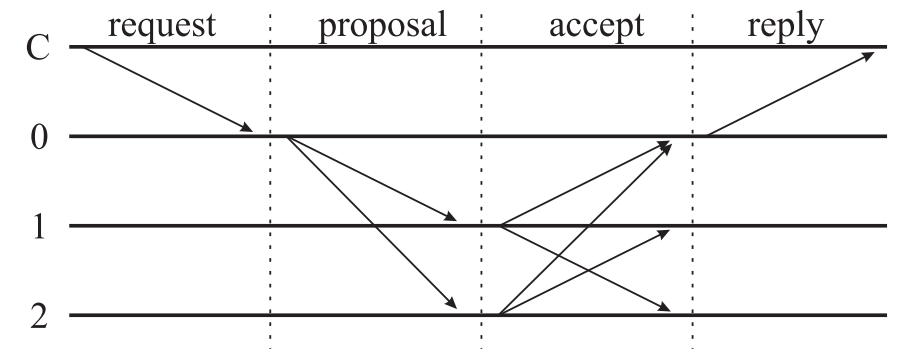
\includegraphics[width=.65\linewidth]{img/paxos}
    \caption{Diagram of a normal case SMR operation}\label{fig:paxos}
\end{figure}
\paragraph{Normal case operation.}
We follow the multi-Paxos protocol~\cite{paxos_simple,paxos_engineering},
where there is a component of the protocol that elects a stable
leader replica, guaranteeing that only that replica can propose
the sequencing of new operations while it remains the leader.
That sequencing corresponds to the normal case operation, which
is described in the pseudocode in Figure~\ref{fig:smr-update},
and is depicted in Figure~\ref{fig:paxos} (following the protocol
description from~\cite{paxos_builders}). In summary, the leader
replica proposes a sequence number for incoming client requests,
and this sequencing must be accepted by a quorum of replicas (a
majority in Paxos), who validate that this sequence number had
not been assigned yet. Once such a majority is gathered, replicas
execute the client operation in that order and the leader
replicas replies with the output of the operation to the client.

\if 0
\begin{enumerate}
    \item A client sends the operation $op$ to be executed to the leader;
    \item The leader assigns the operation a slot number $s$ on the
      sequence of state machine commands (based on the next free slot in
      its local sequence);
    \item The leader sends $prepare(s, op)$ to all replicas,
        logging the sending of this message in persistent storage
        before initiating its transmission;
    \item If a replica has slot $s$ open in its sequence of commands, it sends an
        $accept(s, op)$ to all replicas, also logging the accept
        message persistently before sending it.
    \item A replica marks a slot as accepted when it receives
      the $S_Q$ matching accepts for that slot.
\end{enumerate}
\fi

Our protocol follows directly from this protocol
description~\cite{paxos_builders}, modifying only the quorum size
when gathering the quorum of accept messages. When moving from
majoriy quorums to the separate quorum
types, we need to observe that a Paxos round is both reading and writing
the current state of the Paxos protocol. This is because it must
read that the slot that is being proposed is not yet taken, and
at the same time record the fact that the slot becomes taken and
cannot be used in subsequent proposals. Thus, majorities are
replaced with superquorums in the \ac{RR}-tolerant version of
Paxos.


\paragraph{Leveraging the \ac{RR} model.}
So far, the protocol adaptation does not leverage the
small read quorums enabled by the \ac{RR} model. Even
read-only operations are serialized in the state machine, and as
such need to update the system state, namely to fill the position
in the sequence of operations.

To leverage small read quorums, we adapt the read-only
optimization described in some protocols such as PBFT~\cite{pbft} or
the Paxos description by van Renesse and Altinbuken~\cite{pmmc}.  In
this optimization, the client contacts a read quorum with an
\textsc{optimized-read} message, asking for the
result of executing the read-only command against current state of the
replicas. If the replies are unanimous, the client can return the
value.

Applying this optimization requires careful reasoning to avoid
violating the linearizable semantics of the protocol,
particularly in the context of partially intersecting quorum
systems. To understand why, consider the possibility of two
successive read operations, $r_1, r_2$, where $r_1$ ends before
$r_2$ begins, and that use quorums $Q_{R1}$ and $Q_{R2}$
(respectively) and execute concurrently with a write $w$ that
gathers a quorum of accepts $Q_W$. In this case, and given
property \textbf{I2} (read quorums may not intersect), $r_1$ may
see $w$ as being complete in a read quorum, but $r_2$ only
contains replicas that have not yet gathered a write quorum of
accepts for $w$, since those replicas might have sent but not yet
received the necessary number of accepts. This would violate
linearizability since $r_1$ precedes $r_2$ in real time but,
given their outputs, they cannot be linearized in that order.

This is yet another occurrence of a split brain scenario, but
the solution in this situation is different: instead of
confirming a written value via stabilization, we abort the
optimized read when it is possible that another value has been
written to the state machine, falling back to reading using a
state machine operation. A replica can detect this situation if
it has sent an $\textsc{accept}$ message for a slot
higher than the last executed operation (as it indicates the
possibility of another read quorum with a different value). If no
replicas in a read quorum have done this, then no other operation
has concluded (\textbf{I1}). As was the case in the register
protocol adaptation, this mechanism can be skipped in the case of
fully intersecting quorum systems.

\paragraph{Proof sketch.}
Just as in the \ac{ABD} protocol, we sketch the proof based on
the existence of a total order for the operations that is
consistent with both the output of operations and the real time
order of request execution and replies~\cite{nancy-book}. This
total order is built in the same manner as before, i.e., it is
given by the slot number $s$, breaking ties by having read-only
operations succeeding both the most recent read/write operation
reflected in the reply and read-only operations with the
same slot number that precede them in real time. By the
construction of the protocol, this order is consistent with the
results that are output to the client, since the replies reflect
the execution of the preceding sequence of state machine commands.
The proof for that the order is consistent with
the real time order of requests is straightforward for the
non-optimized protocol but more subtle for the case where one or
both of the requests follow the read-only optimization.
In this case, a later read-only operation cannot revert to a
previous state because of the protocol feature that replicas with
pending accepts deny an optimized read.  This ensures that
it is impossible to have a more recent state
that could have been reflected by a preceding read/write or
optimized read, because intersection property \textbf{I1} implies
that at least one node from the read quorum in the later read
would have sent the accept for the operation that created the
more recent state, since its execution requires a write quorum of
accepts.


\subsection{Security Properties}\label{ssec:sec_prop}
\bsd{Consider moving to chapter 4}\rr{maybe, discuss}
If the threat model for \acp{TEE} explained in
Section~\ref{ssec:tee_motivation} holds, the protocols described in this
section achieve freshness, integrity and confidentiality.
Confidentiality of the overall system is inherited trivially from the
\ac{TEE} fault model. Integrity and freshness of data follow from the
correctness of the protocols, guaranteed by their linearizability
proofs (present in full in the Appendix). These proofs rely on
the intersection properties of the quorum system, in particular
that they mask the rolled back replicas. Moreover, they assume the
\ac{RR} model applies to the replicas, which is
guaranteed by encapsulating replicas inside the \acp{TEE}. Crucially,
the usage of \acp{TEE} (which have integrity of the computation)
guarantees that the protocol is followed by all replicas (even if
they have stale data).

\section{Evaluation of \ac{TEE} replication protocols}

We evaluate our various implementations based on the \ac{RR}
model using micro-benchmarks for protocol implementations and
benchmark workloads for the full system built using those
protocols. Our experiments attempt to answer the following
questions:

\begin{enumerate}
    \item How significant is the effort to change a \ac{CFT}
        implementation to support the \ac{RR} model?
        (\S\ref{ssec:implementation_effort})
    \item How do the protocols based on the \ac{RR} model
      compare with their counterparts based on the Crash and Byzantine
      fault models? And how does that performance behave under increased load?  (\S\ref{ssec:eval_quorum})
\end{enumerate}

\subsection{Implementation}\label{ssec:impl}

We implemented both the read/write register and SMR protocols in
the three fault models (crash, \ac{RR}, and Byzantine) in Intel
SGX (version 1), using C++. All prototypes were implemented using
the same codebase, limiting the changes between prototypes to
what was required by the protocols (e.g.\ extra protocol steps,
different quorums). The PBFT~\cite{pbft} implementation uses the
standard optimization of using MACs instead of digital
signatures.

SGX applications have two separate regions of memory: the
application (untrusted) and the enclave (trusted). In all cases,
the application code comprises 1KLoC (mostly for bootstrap and
interfacing with the local \ac{OS}). All replicas are implemented
using a single-threaded event loop, and take between 4.5KLoC for
the distributed register and 4KLoC for \ac{SMR}. Additionally, the client libraries, which
interact with the replicas take up 5KLoC (distributed
register) and 4KLoC (\ac{SMR}).

It is important to observe that, since in the \ac{TEE} use case,
replicas cannot generally trust clients to execute the protocol
code correctly, our prototypes implement the driver code
collocated with the replicas. This is only relevant in the
distributed register case, since there is no client-side protocol
to be executed in Paxos. A possible alternative would have been
to implement a \ac{TEE} library that drives the register
protocol, which all replicas would remotely attest. We chose
not to do this, since this approach has wider applicability
(e.g.:\ it allows clients that do not run in \ac{TEE}-enabled
platforms to interact with a \ac{TEE} replicated system).
\rr{need to explain better}


\subsection{Experimental Setup.}
We ran our experiments using 7 machines  with
Intel$^\text{\textregistered}$ Xeon$^\text{\textregistered}$ E-2174G
processors running Debian Linux version 4.19 to run the replicas,
plus a machines equipped with an Intel$^\text{\textregistered}$
Xeon$^\text{\textregistered}$ Platinum 8260M processor running Debian
Linux version 5.4 to execute the clients.
%
All machines were connected to same local network. To emulate
different deployment scenarios, we developed
\texttt{sloth}\cite{sloth}, which internally uses
\texttt{netem}\cite{netem} to implement a network topology from a
high-level JSON description. We considered two deployment
scenarios in these experiments: a local area network where all
machines are connected by links whose latency follows a normal
distribution with mean $1$ms and standard deviation of $\sigma =
0.5$ms (which we will refer to as the $1$ms topology); the
deployment scenarios of Figure~\ref{fig:deployments}; and a
geo-replication scenario, based on the measured the link
properties (latency and bandwidth) between several AWS
EC2~\cite{ec2} instances (t2.medium or t3.medium types), located
in regions spread across the globe (AWS topology). This setup
ensures flexibility and experimental reproducability.

In our result graphs, each data point represents the median
measurement over $3,000$ requests (except throughput numbers as
described belows) and the error bars show the $5^{\text{th}}$ and
$95^{\text{th}}$ percentiles.

\subsection{Code changes}\label{ssec:implementation_effort}

Changing a \ac{CFT} implementation to reflect the protocol changes
required by the \ac{RR} model requires low programming
overhead. Mainly, this consists of handling the restart
flag, the existence of different quorums and the mechanisms to
prevent split brain (e.g.\ the stabilization in the register
protocol). For the read/write register prototype, we
modified $72$ LoC and added $211$ new ones. For the SMR
prototype, we modified $24$ LoC and added $28$. \rr{clarify as
per reviews}

\begin{figure}[t]
    \centering
    \begin{minipage}[t]{.49\linewidth}
        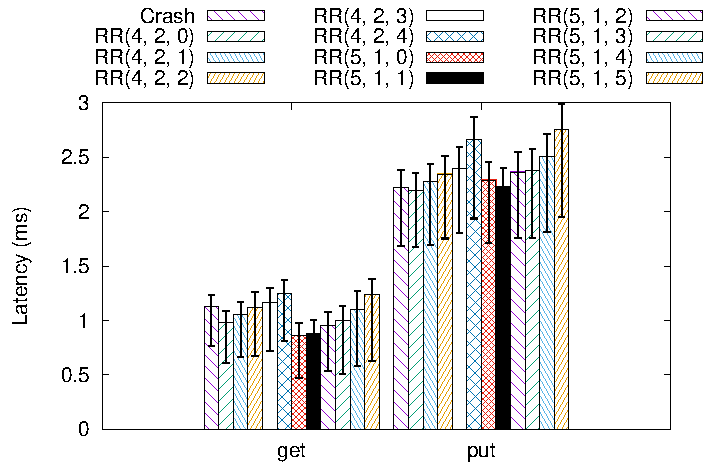
\includegraphics[width=\linewidth]{teem_results/protocol/1ms/parameter/reg_parameter}
        \caption{Read-write register}\label{fig:1ms_reg_lat_conf}
    \end{minipage}
    \begin{minipage}[t]{.49\linewidth}
        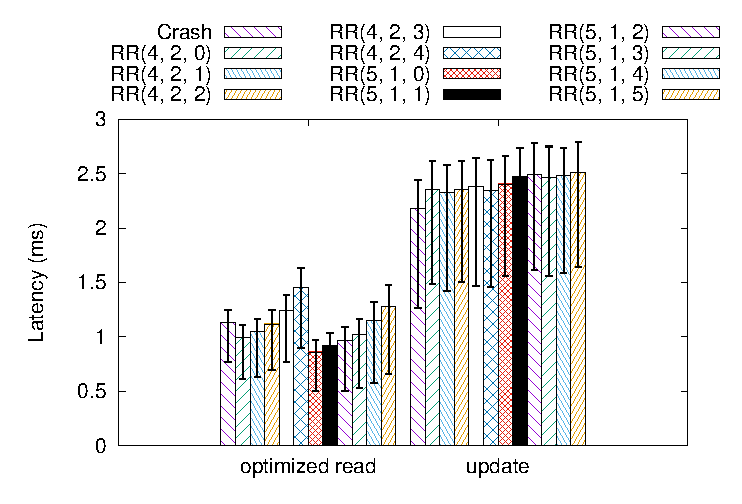
\includegraphics[width=\linewidth]{teem_results/protocol/1ms/parameter/smr_parameter}
        \caption{State machine}\label{fig:1ms_smr_lat_conf}
    \end{minipage}
    \caption{Latency for
    different configurations and models in the $1$ms topology. \ac{CFT} uses
    $F=3$ and $RR(M_R, F, s)$ denote \ac{RR} with parameters $M_R$ and
    $F$, with $s$ restarts.}
\end{figure}\label{fig:protocol_parameter_lat}

\begin{figure*}[th!]
    \centering
    \begin{minipage}[t]{0.24\linewidth}
        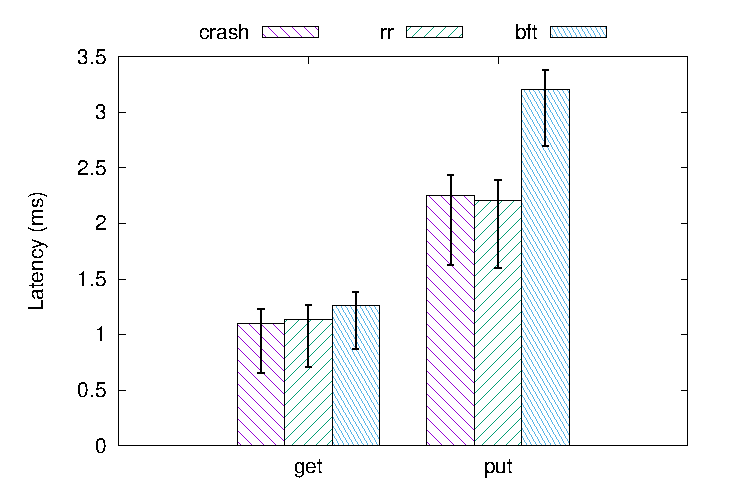
\includegraphics[width=\linewidth]{teem_results/protocol/1ms/lat/1ms_reg}
        \caption{Read-write register ($1ms$)}\label{fig:1ms_reg_lat}
    \end{minipage}
    \begin{minipage}[t]{0.24\linewidth}
        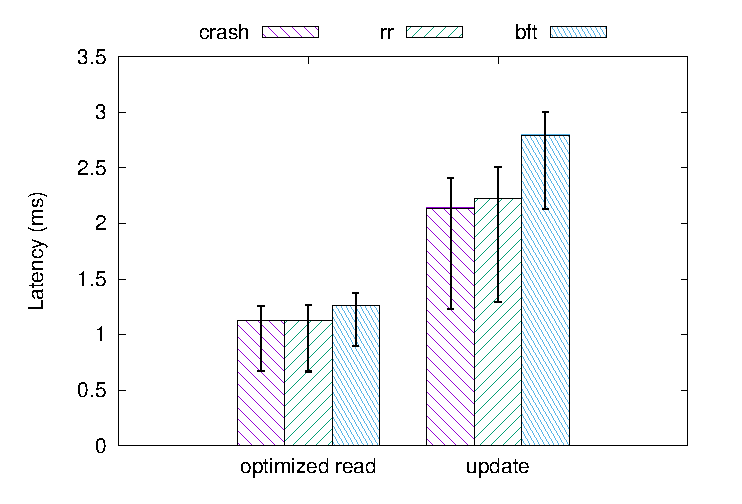
\includegraphics[width=\linewidth]{teem_results/protocol/1ms/lat/1ms_smr}
        \caption{State machine ($1ms$)}\label{fig:1ms_smr_lat}
    \end{minipage}
    %\vskip 0.1cm
    \begin{minipage}[t]{0.24\linewidth}
        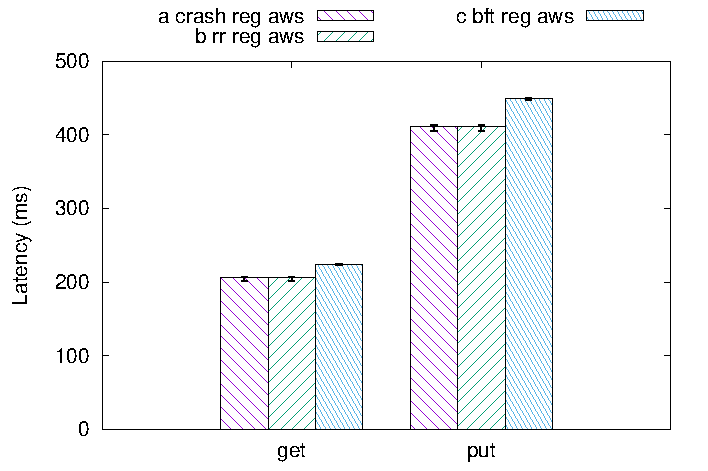
\includegraphics[width=\linewidth]{teem_results/protocol/aws/aws_reg}
        \caption{Read-write register (AWS)}\label{fig:aws_reg_lat}
    \end{minipage}
    \begin{minipage}[t]{0.24\linewidth}
        \centering
        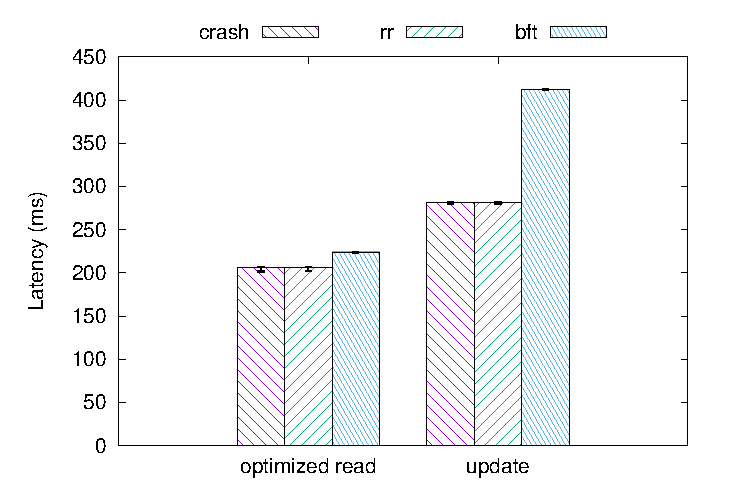
\includegraphics[width=\linewidth]{teem_results/protocol/aws/aws_smr}
        \caption{State machine (AWS)}\label{fig:aws_smr_lat}
    \end{minipage}
    \caption{Operation latency for different protocols in
    different network topologies}
\end{figure*}\label{fig:protocol_lat}

\begin{figure*}[th!]
    \centering
    \begin{minipage}[t]{0.45\linewidth}
        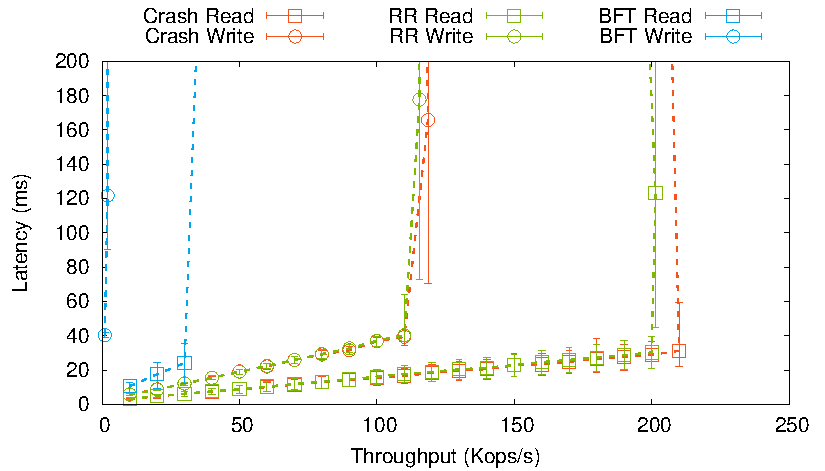
\includegraphics[width=\linewidth]{teem_results/protocol/1ms/reg-tput/result/reg}
        \caption{Read-write register}\label{fig:reg_tputlat}
    \end{minipage}
    \begin{minipage}[t]{0.45\linewidth}
        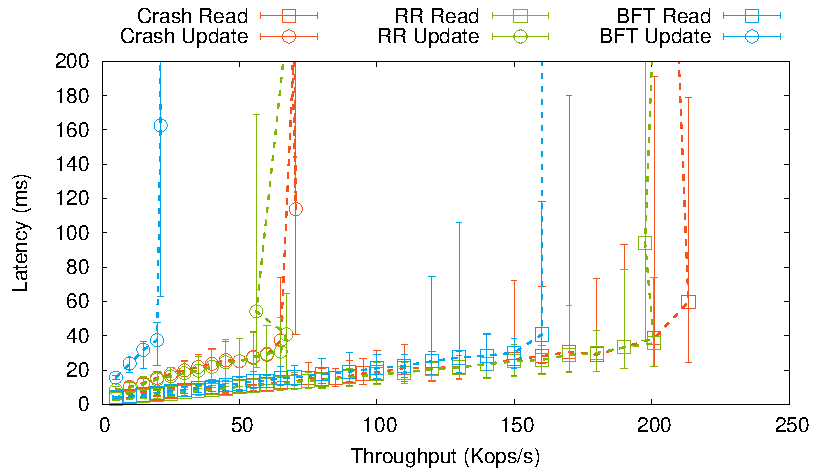
\includegraphics[width=\linewidth]{teem_results/protocol/1ms/smr-tput/result/smr}
        \caption{Replicated state machine}\label{fig:smr_tputlat}
    \end{minipage}
    \caption{Throughput-Latency curve for different protocols}
\end{figure*}


%-------------------------------------------------------------------------------
\subsection{Protocol performance in different models}\label{ssec:eval_quorum}
%-------------------------------------------------------------------------------

Next, we focus on comparing the performance of both classes of protocols under different
fault models.
%
We compare our adapted read-write register with the original ABD
protocol and the \ac{BFT} read-write register protocol described
in~\cite{Malkhi:Reiter:BQS:98}. For SMR, we compared our protocol with
Paxos as described by Kirsch and Amir~\cite{paxos_builders} and the
PBFT protocol~\cite{pbft}. We fixed the fault parameter, $F= 2$ across
quorum systems (with $M_R=2$ in the \ac{RR} quorum system),
yielding quorums with $3$ replicas in the crash and
\ac{RR} models and $5$ replicas in the Byzantine model. The
parametrizations are summarized in
Table~\ref{table:quorum_sizes}, along with the resulting quorum
and system sizes.

\begin{table}[b]
    \centering
    \begin{tabular}{|r || c | c | c || c | c |}
        \hline
        \textbf{Model}       & N & F & $M_R$ & $R_Q(s = 0)$ & $W_Q$\\ \hline
        \textbf{\ac{CFT}}         & 5 & 2 &   &   3   &   3  \\
        \textbf{\ac{RR}} & 5 & 2 & 2 &   3   &   3  \\
        \textbf{\ac{BFT}}         & 7 & 2 &   &   5   &   5  \\ \hline
    \end{tabular}
    \caption{Parameters required by different fault models.}\label{table:quorum_sizes}
\end{table}

The results in Figures~\ref{fig:1ms_reg_lat}-~\ref{fig:aws_smr_lat}
reflect the differences between the different fault models.  We
observe that larger quorums make the operations slower, since the
operation latency is bound by the latency of the slowest replica in
the quorum. Notably, in both cases the performance of the
\ac{RR} protocols matches that of the \ac{CFT} ones, which is to be
expected as they have equally sized quorums.

Next, we measure how the performance of different quorum systems
degrades as the system load increases, as well as the maximum
throughput obtained. In the experiment, we vary the offered load by
increasing the number of concurrent client requests of a single type,
and measure both latency and throughput, keeping the message and
object sizes fixed. Throughput is measured by
counting the number of replies obtained per time interval.  Each
data point corresponds to the median latency or throughput over $5$
seconds of continuous load after a warm-up.
%

Figure~\ref{fig:reg_tputlat} shows that
the read-write register with the \ac{RR} configuration achieves a maximum
throughput of approximately $200$ and $110$ Kops/s for reads and
writes, respectively, being matched by the \ac{CFT} register, as
expected. The \ac{BFT} register has significantly lower throughput,
peaking at approximately $30$ and $2$ Kops/s for reads and
writes.

In Figure~\ref{fig:smr_tputlat} we can again observe that the \ac{CFT} and
\ac{RR} protocols behave comparably, peaking at
approximately $65$ and $200$ Kops/s for updates and optimized
reads, respectively. The \ac{BFT} protocol peaks at $20$ and $160$
Kops/s for updates and optimized reads, respectively. This is due
to both larger quorums and the extra protocol round of PBFT.

In all cases, the throughput becomes bounded by the CPU: the
amount of request that nodes need to process exceeds the
capability of the hardware. In the \ac{BFT} protocols, there are
both more replicas and more rounds, which equates to more
messages to be processed and, by extension, lower
throughput.\rr{how do you know?}

In the preceding experiments, the crash and \ac{RR} protocols
used equally sized quorums, and as such had very similar
performance. However, as discussed in Sections~\ref{sec:model}
and~\ref{sec:protocol}, the \ac{RR} model has asymmetric quorums,
which lends itself to faster reads (at the expense of slower
writes). Moreover, in the preceding experiments the number of
restarts has been set to $0$, as this is the common case. To
better explore the configuration space of \ac{RR} quorums and
their performance difference to \ac{CFT}, we reran the latency
experiments from
Figures~\ref{fig:1ms_reg_lat}--\ref{fig:1ms_smr_lat}, but with
different quorum configurations. In
Figures~\ref{fig:1ms_reg_lat_conf}--\ref{fig:1ms_smr_lat_conf},
we can observe that, by leveraging the smaller quorums of
\ac{RR}, read operations become faster than their equivalents in
\ac{CFT}, at the expense of more expensive writes. Moreover, as
the number of restarts increases, the difference to \ac{CFT}
shrinks, and eventually \ac{CFT} reads outperform \ac{RR}, in the
uncommon case where most replicas have just restarted and have
yet to run their recovery protocol. Similarly, as the number of
restarts increases, write/update operations also become more
expensive (as they require read quorums in some steps).

Overall, the results show that \ac{RR} has very close performance
to \ac{CFT}, while offering rollback protection and better read performance
in some configurations, in the common case with few restarts.
Compared to \ac{BFT}, \ac{RR} offers significantly better performance
due to its smaller quorums.

\section{Discussion: Generalization of the \ac{RR} model}\label{sec:discussion}

A key insight of the \ac{RR} fault model is that it is possible
to detect, with false positives, when non-crash faulty behaviour
has ocurred in the system. With this suspicion, plus a deployment
specific hard limit on the number of nodes that can actually
exhibit this faulty behaviour at the same time, we have derived
the \ac{RR} quorum systems and associated protocols. The \ac{RR}
fault model can be considered a generalization of the crash fault
model (i.e.\ when $M_R = 0$). It is interesting to consider
whether it can itself be further generalized to faulty behaviour
other than rollbacks.

From a technical point of view, this is definitely possible.
Provided that there exists a \emph{suspicion function} that
detects, with false positives, when non-crash faulty behaviour
has ocurred while reading the system, one could reuse the derivation
of quorum systems presented in this chapter and the associated
protocols. This would even generalize to the Byzantine model, as a
trivial function which always suspects that a fault
might have happened would correctly capture Byzantine behaviour.
Curiously, the quorum system derived using this function is the
one described by UpRight~\cite{upright}. Another trivial function
would never suspect non-crash behaviour, being valid in the crash
fault model.

However, outside these trivial suspicion functions and the
suspicion function that simply reports the suspicion flag from
\ac{RR} nodes, we have not been able to craft functions that
present some usefulness. Although this does not mean, by any
means, that they do not exist, our experience points to the
suspicion function \new{not being a particularly good} abstraction for capturing
intermediate fault models between the crash and Byzantine other
than the \ac{RR} model.

\cleardoublepage{}

\fancychapter{\ac{TEE} replication using the \ac{RR} model}\label{chap:tee}
\cleardoublepage{}

As we have discussed previously, \acp{TEE} are an interesting
option deploying replicated systems in an untrusted public cloud.
In this chapter, we present the \acf{TEEMS}, a replicated metadata
service for trusted cloud storage. \ac{TEEMS} has a double purpose in
the context of this dissertation: it showcases a practical system
using the \ac{RR} fault model and associated register and
\ac{SMR} protocols and provides the means of enhancing existing
cloud storage systems such that they can be trusted and remotely
attested in the same fault model as \acp{TEE} (and, by extension,
used by them as a persistent storage, with rollback protection).

This chapter is organized as follows.
Section~\ref{sec:teems_design}
provides the motivation and design of \ac{TEEMS}, followed by
Section~\ref{sec:teems_impl}, which describes the implementation
of \ac{TEEMS}. Finally, Section~\ref{sec:teems_eval} presents an
extensive evaluation of \ac{TEEMS} using real-world workloads
across different deployments.

\section{\ac{TEEMS}: Metadata service for trusted cloud
storage}\label{sec:teems_design}


\subsection{Motivation}

\acp{TEE} have enabled services like Azure Confidential
Computing~\cite{azure-conf} and Google Confidential
VMs~\cite{google-confVM}, where Cloud tenants can use compute
services without trusting the platform provider.  However, the
strong security properties from \acp{TEE} do not automatically
extend to cloud storage. To create a cloud-based system with
similar strong security guarantees of \acp{TEE}, it is only
natural to consider using \acp{TEE} as its building blocks. A
\ac{TEE}-encapsulated metadata service, replicated for
availability and fault-tolerance, can maintain encryption keys
and version information for data blobs stored in untrusted Cloud
storage.  By ensuring confidentiality, integrity, and freshness
of the metadata, the service extends the same guarantees to the
encrypted and versioned data blobs. Moreover, by supporting an
atomic update operation on metadata, the service enables
concurrent sharing of data blobs.

This approach needs to be integrated at the replication
level. Fundamentally, even assuming an efficient way for
storing the state of a single \ac{TEE}, this solution would still be
unable to support concurrent sharing between multiple \acp{TEE}. This
is because ensuring freshness of a single \ac{TEE}'s own state relies
on persistently storing a monotonic counter~\cite{ariadne,rote,ice}
or a top-level hash~\cite{memoir}, which can only be updated by
the \ac{TEE} itself.  Concurrent sharing of persistent state instead
requires atomic, concurrent updates of state blobs and their
associated metadata (e.g., counter).

We designed and implemented a replicated metadata service called
\ac{TEEMS} (for \ac{TEE}-based Metadata Service) based on the
\ac{RR} fault model. \ac{TEEMS}'s replicas can be hosted in a
diverse set of cloud providers for high availability and
resilience.
%
\ac{TEEMS} provides a read/write interface for metadata and guarantees that
readers always receive the metadata (e.g., encryption key) of the most
recent version of a data blob.  \ac{TEEMS} also supports access control
policies for metadata, and therefore allows clients to selectively
share the associated data blobs.  The service therefore enables
trusted storage services that extend the strong guarantees of today's
\ac{TEE}-based cloud compute services to persistent storage.

\subsection{\ac{TEE}-grade cloud storage with \ac{TEEMS}}

Clients can use \ac{TEEMS} to lend untrusted cloud storage \ac{TEE}-level
guarantees, by using the API in Table~\ref{tab:teems}.
\ac{TEEMS} maintains metadata for each data blob, i.e. a short summary of
the most recent version of a data blob, namely its hash and encryption
key. The encrypted data blob is then stored in an ordinary cloud
storage service. This extends the integrity, confidentiality,
freshness and selective concurrent sharing properties of the
metadata service to the cloud storage, while relying on the cloud
service only for storage and availability.

\begin{table}[!t]
    \centering
    \renewcommand{\arraystretch}{0.9} % this reduces the vertical spacing between rows
    \begin{small}
    \begin{tabular}{rll}
        \hline
        Return Value && {Command and Arguments}\\
        \hline
        \{\lArg{status}\} &\eq& {\sysC{teems-init}(\lArg{client ID})}\\
        \{\lArg{status}\} &\eq&{\sysC{teems-close}}()\\
        \{\lArg{status}\} &\eq&{\sysC{teems-write}}(\lArg{id}, \nArg{val})\\
        \{\lArg{status}, \nArg{val}, \lArg{ver}\} &\eq&{\sysC{teem-read}}(\lArg{id})\\
        \{\lArg{status}\} &\eq&{\sysC{teems-delete}}(\lArg{id})\\
        \{\lArg{status}\} &\eq&{\sysC{teems-change-policy}}(\lArg{id}, \lArg{policy-code})\\
        \hline
    \end{tabular}
    \end{small}
    \caption{\ac{TEEMS} Interface}\label{tab:teems}
\end{table}

Concurrent sharing of mutable data fundamentally requires a
read-modify-write operation (i.e., some form of \ac{SMR}).
However, state machine operations are more expensive than
read/write register operations. \ac{TEEMS} minimizes the use of
state machine operations in situations where writers typically
perform multiple updates of a data blob before other writers
perform an update as follows.  We mediate access to the metadata
via single writer policies, and implement policy changes via the
more expensive read-modify-write state machine operation. Simply
reading and updating the metadata of a blob (by the current
writer) is implemented using efficient distributed register
operations.  This approach ensures safe concurrent sharing of
data blobs while minimizing the more expensive policy changes to
cases when the writer for a blob changes. The full \ac{TEEMS}
interface is summarized in Table~\ref{tab:teems}.

Storage operations involve the following sequence of steps.  When an
operation to write a new data blob $d$ associated with id $i$ is
invoked, the client library starts by generating a symmetric
encryption key $k$. In our implementation, we use an authenticated
encryption scheme (AES-GCM), which generates a ciphertext ($\langle d
\rangle_k$) and a MAC ($MAC(d)$) of $d$.
%
The encrypted object and corresponding MAC are then stored in one
or more untrusted cloud storage services, under a randomly
created identifier $i_{store}$. Let $a$ be the access control
list for the newly stored data blob $d$. After the data has been
successfully written to untrusted storage, the library contacts
the \ac{TEEMS} metadata service to update the metadata for id $i$:
\[ \langle i,k,a,i_{store},MAC(d) \rangle   \]
%
The write operation concludes successfully after both the data
write and the metadata update complete. Finally, the library
deletes earlier versions of the blob from the data store.

When a read for id $i$ is invoked, the client library starts by
querying the \ac{TEEMS} service for the most recent version of
the metadata associated with the id $i$. After retrieving the
tuple $\langle i,k_i,i_{store},MAC(d_i) \rangle$, the client
library then uses the id $i_{store}$ to retrieve the encrypted
data from untrusted storage. This encrypted data $\langle
d'\rangle_{k_i}$ is read and then decrypted using $k_i$,
obtaining $d'$ and $MAC(d')$. Finally, its integrity  is
validated by comparing $MAC(d')$ and $MAC(d_i)$.

Finally, the access to the untrusted storage can be optimized by
employing caching at the client. We can either cache full blobs (to
avoid having to access the untrusted store) or name hints (for
enabling parallel access to the metadata service and the untrusted
store).  In either case, the metadata always has to be fetched and
compared with the cached or retrieved version, since only the
\ac{TEEMS} metadata service can ensure freshness of data blobs.

\subsection{Leveraging different storage protocols}

\ac{TEEMS} implements the metadata read/write operations efficiently using
our \ac{RR}-tolerant ABD protocol (Section~\ref{ssec:abd}).  However,
updating the policies stored by \ac{TEEMS} --- which enables concurrent
 sharing --- requires a read-modify-write operation, because changing
a policy requires reading the policy first to check if the client has
permission to modify it.  Therefore, policy changes are implemented
using the \ac{RR}-tolerant SMR protocol
(Section~\ref{ssec:paxos}).  This combination of protocols allows us
to achieve both efficient reads and writes in the normal case, and
concurrent write sharing via atomic policy changes through state
machine updates.

In this design, the state of our state machine is an epoch number
and an associated policy description. Crucially, the
epoch number is also readable by the read/write protocol. As
such, a policy change is a state machine operation which
evaluates the current policy, replacing it with the proposed
policy and incrementing the epoch number, if such permission is
granted. The epoch number increment is then immediately
visible to register operations.

\begin{figure}[t]
  \begin{small}
    \textbf{Write Metadata (key $k$, value $v$)}

    \begin{enumerate}[itemsep=0pt,parsep=0pt]

        \item \textbf{smr\_get\_policy ($k$)}

        \item \textbf{if} $eval(policy) == \textsc{access denied}$ \textbf{then}\\
            \tabto{.5cm}    \textbf{return} $\textsc{access denied}$

        \item \textbf{register\_write ($k$, $v$, $epoch$)}

        \item \textbf{if} $\textsc{epoch changed}$ \textbf{then}\\
            \tabto{.5cm}    \textbf{restart operation}

        \item \textbf{return} \textsc{Success}
    \end{enumerate}

  \end{small}
  \caption{Slow but trivially correct mixing of the protocols.
    The read operation is in all aspects similar.}\label{fig:teems_slow_correct}
\end{figure}

\begin{figure}[t]
  \begin{small}
    \textbf{Write Metadata (key $k$, value $v$)}

    \begin{enumerate}[itemsep=0pt,parsep=0pt]

        \item \textbf{smr\_optimized\_get\_policy ($k$)} in
            parallel with \textbf{register\_get\_version ($k$)}

        \item \textbf{if} $smr\_optimized\_get\_policy$ fails \textbf{then}\\
            \tabto{.5cm}    \textbf{fallback} to slow operation

        \item \textbf{if} $eval(policy) == \textsc{access denied}$ \textbf{then}\\
            \tabto{.5cm}    \textbf{return} $\textsc{access denied}$

        \item \textbf{broadcast} \textsc{Write Replica} ($epoch$, $new\_ts$, $v$) and wait for $W_Q$ replies;

        \item \textbf{return} \textsc{Success}
    \end{enumerate}

  \end{small}
  \caption{By overlapping (and piggybacking) the optimized read
    to the state machine to get the policy and the reading of the
    current timestamp of the register (which is the first step of
    the write protocol), we can run both operations in parallel,
    since writing the value to the register only happens after
    the policy is verified. Note that the read operation can be
    similarly piggybacked (the value is only returned after the
    policy check)}\label{fig:teems_fast_mixing}
\end{figure}


For reads and writes, a slow but trivially correct combination of
the protocols would be to issue a read operation on the state
machine to obtain the policy and then issue the register
operation, retrying if the epoch number has advanced, as described in Figure~\ref{fig:teems_slow_correct}.
The correctness of the combination hinges on the fact that 1) the
policy is correctly read and enforced; and 2) by ensuring the epoch
has not changed between checking the policy and operating on the
register, the policy is guaranteed to be valid for that version of the
object.
% PD I don't think this needs to be pointed out
%There is a danger of a livelock, which would happen if policies were
%being constantly updated (thus forcing constant restarts). This is an
%unlikely usage pattern of a policy change, and can be mitigated, e.g.,
%by requiring that a policy can only be replaced after a certain number
%of register operations succeeded.


%A key insight for performance, which enables fast reads and
%writes in the absence of concurrent policy changes,
We note, however, that the initial phase of the register operation has
the same communication pattern as the optimized read state machine
operation. As such, it is possible to piggyback the optimized read
request with the first phase of the register operation, as shown in
Figure~\ref{fig:teems_fast_mixing}. If the fast policy read succeeds,
the policy is evaluated and the operation proceeds.  Otherwise, the
system falls back on the slow path above. The optimization is correct
because it is equivalent to the slower combination: the operation
succeeds only if the policy is enforced and the register sub-operation
only succeeds if it happens within the epoch of the policy.

The client side policy evaluation and protocol execution require
trusted computation, meaning the implementation needs to either
rely on a \ac{TEEMS} replica as a proxy or on a client-operated \ac{TEE},
attested by the replicas. In our description, as well as in our
prototype implementation, we chose the former.

\subsection{Security Properties}

\ac{TEEMS} ensures the confidentiality, integrity, and
freshness of stored data blobs, due to the correctness of the
underlying protocols, as discussed in
Section~\ref{ssec:model_sec_prop}. However, the untrusted storage is relied
upon for availability of data blobs. For increased availability,
clients may store multiple copies of a data blob (or
erasure-coded fragments) at independent storage providers.
%
\subsection{Deployment scenarios}

\begin{figure}[t] \centering
        %
\includegraphics[width=.32\linewidth]{ps/diag-1}
        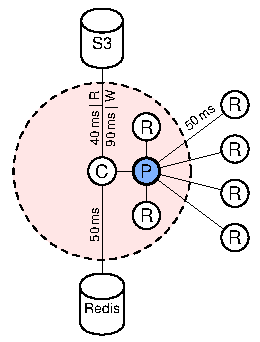
\includegraphics[width=.32\linewidth]{ps/diag-2}
        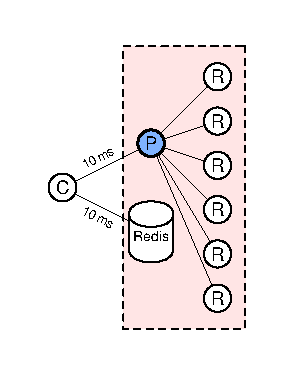
\includegraphics[width=.32\linewidth]{ps/diag-3}\\
        (a) \hspace{2.7cm} (b)
    \caption{Deployment scenarios: (a) cloud client (with either
    Redis or S3), (b) collocation center with Redis. The shaded area represents a
    LAN (or a data center). Latencies will be used in the
    evaluation (in the case of S3, $R$ represents the latency of
    reads and $W$ the latency of writes). $C$ is the client, $R$ is a replica and $P$ is the proxy replica.
    }\label{fig:deployments}
\end{figure}


To minimize the chance of correlated faults of individual metadata
servers, each replica can be at a different location, depending on the
deployment scenario. For example, the \ac{TEEMS} replicas may be
distributed over multiple administrative domains to make it less
likely that several of them can be rolled back at any given time. One
way to achieve this distribution is to colocate some replicas with a
client in a data-center, with the remaining replicas in other
administrative domains (Figure~\ref{fig:deployments}a).  In another
example scenario, clients execute on their own premises and wish to
share data items stored in the Cloud with other clients, without
trusting the Cloud. They can use \ac{TEEMS} replicas deployed at a local
collocation center, where subsets can be physically isolated and
operated by independent providers, possibly using storage in the same
center (Figure~\ref{fig:deployments}b).

Depending on their cost and availability needs, clients may opt to
store a single copy on a single cloud storage service provider,
multiple copies on independent providers, or multiple erasure coded
fragments on independent providers. In the common case, a copy or a
small set of fragments can be efficiently retrieved from the nearest
providers.


\section{Implementation}\label{sec:teems_impl}

We implemented the \ac{TEEMS} prototype in Intel SGX (version 1),
using C++. The \ac{TEEMS} servers are implemented using a
single-threaded event loop and 6KLoC (\ac{TEEMS}). Additionally,
the client library, which interacts with the replicas and with
the untrusted storage, takes up to 5KLoC (\ac{TEEMS}). We used
Flatbuffers~\cite{flatbuffers} to define our protocol messages
and their serialization, but implemented the secure transport
between the replicas using OpenSSL~\cite{openssl}.

It is important to observe that since in \ac{TEE} replicated
systems replicas cannot generally trust clients to execute the protocol
code correctly, our prototypes implement the driver code
collocated with the replicas. This means that, for instance, a
register write request is first sent to a \ac{TEEMS} server (typically, one
collocated with the client) which acts as a proxy and runs the
two rounds of the protocol. A possible alternative would have been
to implement a \ac{TEE} library that drives the register
protocol, which all replicas would remotely attest. We chose
not to do this, since the former approach has wider applicability
(e.g., it allows clients that do not run in \ac{TEE}-enabled
platforms to interact with a \ac{TEE} replicated system).

All prototypes are open-sourced under the MIT license
and available at \url{https://gitlab.mpi-sws.org/restart-rollback}.

\section{Evaluation}\label{sec:teems_eval}


We evaluate the \ac{TEEMS} prototype based on the \ac{RR} model
using benchmark workloads, aiming to answer the following questions:

\begin{enumerate}
    \item What is the overhead added by \ac{TEEMS} to secure a cloud storage system under different
      deployments?  (\S\ref{ssec:teems_eval_deploy})
    \item What is the performance of this system  when used to store
      metadata for a \ac{KVS} (Redis) under a benchmark
        workload (\ac{YCSB})?
      (\S\ref{ssec:ycsb})
\end{enumerate}

\paragraph{Experimental Setup.}
We ran our experiments using 7 machines  with
Intel$^\text{\textregistered}$ Xeon$^\text{\textregistered}$ E-2174G
processors running Debian Linux version 4.19 to run the replicas,
plus 2 machines equipped with Intel$^\text{\textregistered}$
Xeon$^\text{\textregistered}$ Platinum 8260M processors running Debian
Linux version 5.4: one of them to execute the clients and the other to
host Redis.
%
We again leveraged \texttt{sloth}~\cite{sloth} to simulate
different network topologies.

In our result graphs, each data point represents the median
measurement over $3,000$ requests and the error bars show the $5^{\text{th}}$ and
$95^{\text{th}}$ percentiles.

\begin{figure*}[t]
    \centering
    \begin{minipage}[t]{0.45\linewidth}
        \centering
        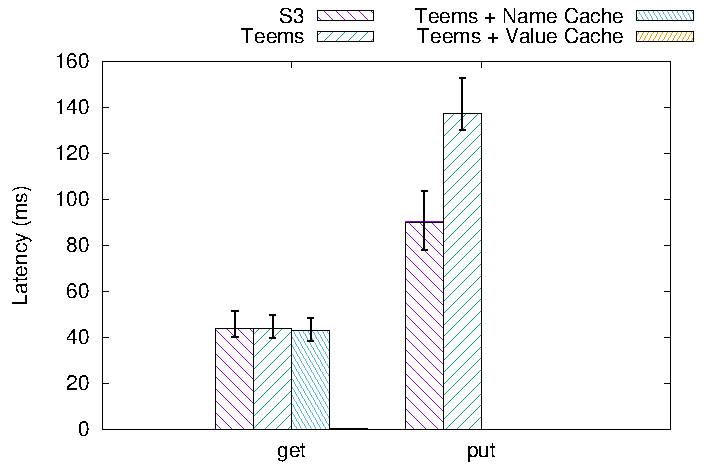
\includegraphics[width=\linewidth]{teem_results/deployment/result/client_cloud_s3}
        \caption{Client in the Cloud w/ S3}\label{fig:cloud_client_s3}
    \end{minipage}
    \begin{minipage}[t]{0.45\linewidth}
        \centering
        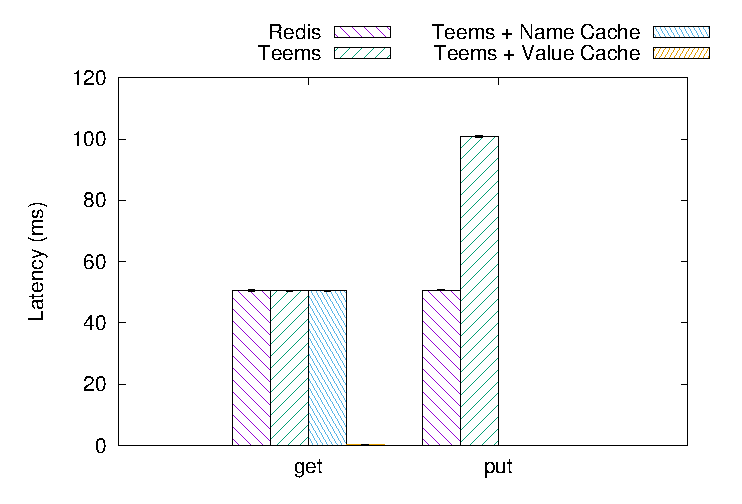
\includegraphics[width=\linewidth]{teem_results/deployment/result/client_cloud_redis}
        \caption{Client in the Cloud w/ Redis}\label{fig:cloud_client_remote_redis}
    \end{minipage}
    \begin{minipage}[t]{0.50\linewidth}
        \centering
        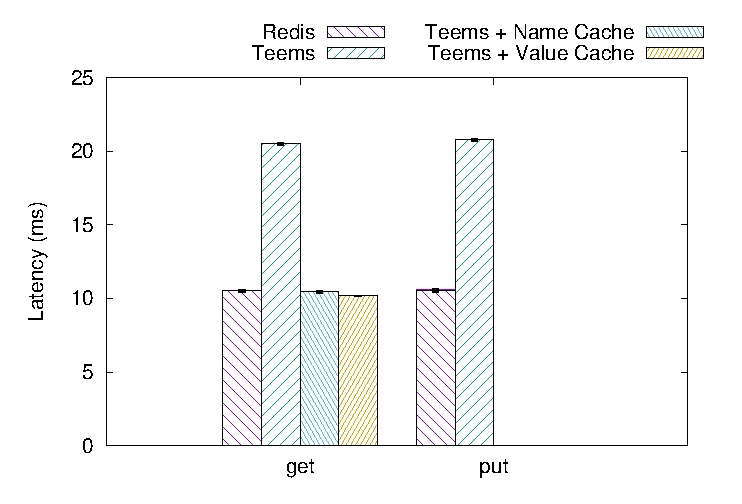
\includegraphics[width=\linewidth]{teem_results/deployment/result/collocation_center}
        \caption{Collocation Center w/ Redis}\label{fig:coloc_redis}
    \end{minipage}
    \caption{Latency in different deployment scenarios. The
    ``s3'' and ``redis'' bars refer to direct accesses to the
    untrusted storage, providing a performance baseline without
    rollback protection. ``teems'' refers to accesses without
    caching. ``teems + name cache'' and ``teems +
    blob cache'' refer to accesses where the name and blob
    caches had a hit, respectively. Caching only applies for
    get requests, and in the cases of
    Figures~\ref{fig:cloud_client_s3} and~\ref{fig:cloud_client_remote_redis}
    the ``value cache'' exists, but is close to zero since the
    cache hit with a local read quorum means there is no network
    latency access in the critical path.}
\end{figure*}



%-------------------------------------------------------------------------------
\subsection{\ac{TEEMS}-based storage}\label{ssec:teems_eval_deploy}
%-------------------------------------------------------------------------------
First, we focus on understanding the performance of our example
application, the  \ac{TEEMS}-based secure storage service, under
different deployments, which differ in the relative location of
the client, the metadata servers, and the type and location of
the untrusted storage. In this set of experiments, our baselines
are the untrusted
storage systems being used in each situation, namely Amazon S3 and an
instantiation of Redis on our local cluster, to which we optionally
add a variable  latency on the
access link.

We consider three representative deployment scenarios, illustrated in
Figure~\ref{fig:deployments}.

\paragraph{Client in the Cloud.}
In this deployment (Figure~\ref{fig:deployments}a), the client is
co-located with three metadata servers and the remaining four servers
are in another data-center.  We use two variants of storage: a
remote Redis deployment, and S3.

\paragraph{Collocation Center.}
In this scenario (Figure~\ref{fig:deployments}b), all metadata
servers and the Redis deployment are in the same collocation center, being hosted by different cloud
providers.

In both cases, the largest administrative domain has $4$
replicas, while at most $2$ replicas are expected to crash
in a correlated fashion. As such, we consider $M_R = 4$ and $F= 2$.

From Figures~\ref{fig:cloud_client_s3}--\ref{fig:coloc_redis}, we
conclude that: 1) \ac{TEEMS} performance depends heavily on the deployment
scenario (in particular on the existence of local read quorums, which
are enabled by \ac{RR}); 2) name caching is effective at masking
the overhead of accessing the metadata store; 3) blob caching, when
combined with local read quorums, allows for local reads of both data
and metadata, outperforming the baseline.


\subsection{\ac{TEEMS}-based storage running \ac{YCSB}}\label{ssec:ycsb}

Next, we compare \ac{TEEMS} with using only
Redis, on the \ac{YCSB} benchmark workloads. We deployed \ac{TEEMS} in the
Client in the Cloud setting with Redis, using name caches. We use all six core workloads
of \ac{YCSB} (A--F), which have different key distributions and read/write
ratios. The size of the objects varies between 100B and 1KB, depending
on the workload and the overall size of the database is of
1000 1KB objects.
%
The results in Figures~\ref{fig:ycsb_teems} and~\ref{fig:ycsb_redis}
show that writes incur a $2\times$ overhead, which is expected since
the Redis access must be preceded by the \ac{TEEMS} metadata access. In
contrast, reads perform comparably to the baseline, due to local
read quorums and effective usage of the cache.

\begin{figure}[t]
    \centering
    \begin{minipage}[t]{0.49\linewidth}
        \centering
        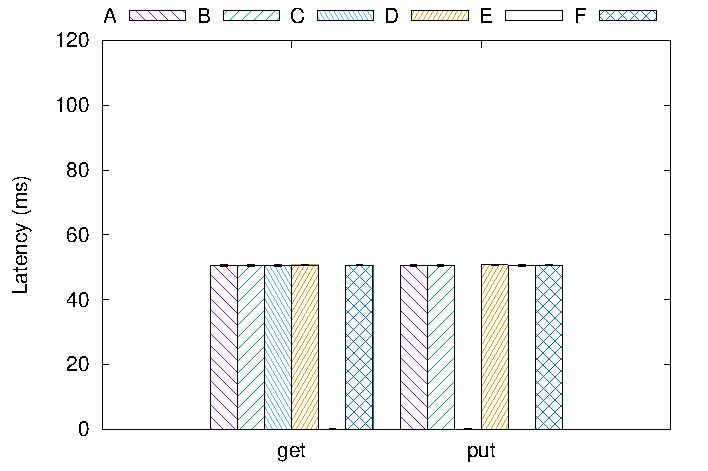
\includegraphics[width=\linewidth]{teem_results/deployment/result/ycsb_redis}
        \caption{Redis baseline}\label{fig:ycsb_redis}
    \end{minipage}
    \begin{minipage}[t]{0.49\linewidth}
        \centering
        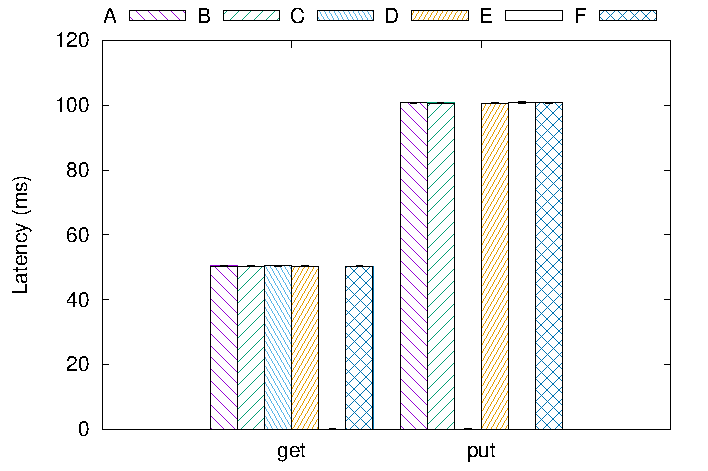
\includegraphics[width=\linewidth]{teem_results/deployment/result/ycsb_teems}
        \caption{\ac{TEEMS} + Redis}\label{fig:ycsb_teems}
    \end{minipage}
    \caption{Latency with \ac{YCSB} workloads}
\end{figure}


\cleardoublepage{}

\fancychapter{Leveraging the \ac{RR} model in distributed storage}\label{chap:storage}
\cleardoublepage{}

In this chapter, we will present the \acf{R2-S2}, a replicated
\ac{KVS} based on LevelDB~\cite{leveldb}, a single node \ac{KVS}
implemented using  \acp{LSM-tree}~\cite{lsm}. We have developed
\ac{R2-S2} to showcase the broad applicability of the \ac{RR}
model by using it in a non-security context, without \acp{TEE}.

The motivation for \ac{R2-S2} is presented in
Section~\ref{sec:r2s2motivation}, followed by its design in
Section~\ref{sec:r2s2design}. We present guidelines for system
parameterization in Sections~\ref{sec:r2s2parameterization}.
A preliminary evaluation is presented in Section~\ref{sec:r2s2evaluation}.

\section{Motivation}\label{sec:r2s2motivation}
Batching multiple small write operations to a block-oriented storage device into a
single large one is a known mechanism to increase its throughput.
To achieve this batching, one has to wait for an adequate amount
of contiguous data to write, which introduces a delay in the
operation. Alternatively, once the data to write is present in
an in-memory buffer (soft state) the system could return to the
client. This opens the possibility of data loss, if the system
crashes before effectively synchronizing this data to the persistent
storage device.

% 5: replication should be able to partially mask this
%
% note: we can introduce the difference between persistent replicated
% storage systems and volatile replicated storage systems
This problem is propagated as is to current persistent replicated storage
systems: the throughput of the system is limited by the
throughput of the storage devices of the replicas. To avoid this
performance penalty, some replicated systems consider data to be persisted if it is
present in volatile memory at a sufficiently large subset of replicas~\cite{pbft}
(i.e., persistence through replication). Such an approach is not
consensual, with other authors insisting that data must be
present in stable storage to be considered
persisted~\cite{bolosky:paxos}.

% Question whether this needs to be a dichotomy
We argue that these two properties --- performance and
durability --- do not need to be mutually exclusive. Instead, we
aim to combine both into a system that offers the throughput from
the solutions that persist in the background with the high
durability from systems that persist before replying to
requests.

% We present a new replication strategy
To this end, we present a novel replication strategy based on
carefully and strategically mixing both approaches, leveraging
\ac{RR} quorum systems. Instead of issuing the write
requests symmetrically to all replicas, as is customary, we can
strategically signal to certain replicas to synchronize to
persistent storage before replying while allowing others to
acknowledge the write eagerly, thus mixing both approaches. This
key insight allows us to take advantage of batching, improving the overall
performance of the system, without relinquishing fault tolerance.
The \ac{RR} fault model captures perfectly replicas that
crash before synchronizing their volatile batches to stable
storage. In this case, these replicas suffer a rollback, but
since they have restarted can flag their suspicion regarding the
freshness of their state.

% 8, 9: challenges
This approach opens a series of challenges. The storage layer
requires careful adaptations to support multiple modes of
operation while offering efficient batching, even on
non-sequential writes. At the replication level, the asymmetry of
operation between replicas introduces the problem of \emph{sync
scheduling}: choosing which replicas synchronize to persistent storage
and which can reply eagerly. This schedule is paramount to
extracting the maximum performance of the system, and offers a
rich design space. Parameterizing a deployment of such a system is
also not obvious. There is a tradeoff to be explored between the
total number of replicas, the number of replicas that synchronize
to disk in the background (and, by extension, the performance of
the system) and the desired availability and reliability of the
system. We present a principled method for this parameterization,
where a system administrator can tune the number of replicas
based on how prone to faults they are and the desired
availability and durability levels.

%%%%%%%%%%%%%%%%%%%%%%%%%%%%%%%%%%%%%%%%%%%%%%
\section{\ac{R2-S2} Design}\label{sec:r2s2design}
%%%%%%%%%%%%%%%%%%%%%%%%%%%%%%%%%%%%%%%%%%%%%%

This section presents the design of \ac{R2-S2}
based on the principle of \emph{asymmetric synchronization}. However,
before discussing our architecture in detail, it is worthwhile to
categorize in a systematic way the three approaches that can be used to synchronize
replica state to stable storage.

\paragraph{Sync immediately.} When receiving an object to write, a
replica immediately writes and flushes the object to stable
storage, issuing the reply afterwards. This prevents batching,
which favours \emph{durability} and \emph{latency} in detriment
of \emph{throughput}.

\paragraph{Batch and wait.} When receiving an object to write, a
replica places the object in a batch and waits for this batch to
be flushed to stable storage. Afterwards, the reply can be
issued. Since there is batching and objects are being persisted
before replying, this approach favours \emph{durability} and
\emph{throughput} at the cost of \emph{latency} (which can be
very large if the batch takes a long time to be filled due to a
lack of writes).

\paragraph{Batch and reply (Move fast and break things).} In this approach,
replicas place the object in the batch (i.e., volatile memory)
and reply immediately. This achieves the best \emph{latency} and
\emph{throughput}, sacrificing \emph{durability} since replicas
can suffer a rollback if they crash and restart.

The state of the art seems to hint at
an impossibility trinity: systems have to pick two between latency,
throughput, and durability. The design goals of \ac{R2-S2} aim to question this
impossibility, by showing that there can be interesting
combinations of these features that, at least, approximate the
best of the three approaches:
\ac{R2-S2}:
\begin{enumerate}
    \item \textbf{Strong Persistence}: data loss should never
        occurr, even in the presence of arbitrary node crashes;

    \item \textbf{Performance}: the architecture should yield
        performance gains compared to
        Approaches A and B\@;
\if 0
    \item \textbf{Generality}: the architecture should be as
        generic as possible. In particular, it should be
        applicable to a variety of replication protocols.
\fi
\end{enumerate}

Note that none of our baselines satisfy all requirements:
approaches A and B achieve
\emph{strong persistence} but not the performance requirement.
Approach C does meet the performance
requirement, but does not satisfy \emph{strong persistence}.

In the remainder of this section, we will describe
\emph{asymmetric synchronization}, the key technique that realizes the
goals prescribed above, and how the architecture needs to
accomodate this paradigm to achieve the best possible
performance.

%%%%%%%%%%%%%%%%%%%%%%%%%%%%%%%%%%%%%%%%%%%%%%
\subsection{Asymmetric Synchronization}\label{ssec:asymmetric_synchronization}
%%%%%%%%%%%%%%%%%%%%%%%%%%%%%%%%%%%%%%%%%%%%%%

Asymmetric synchronization is the key to extracting performance
in \ac{R2-S2}. The core idea is to partition the replica set
into two disjoint subsets: the \emph{volatile set}
$\mathbbm{R}$, composed of the replicas that eagerly reply to the
request before synchronizing to persistent storage (and thus can
suffer a rollback on restart); and the sync set $\mathbb{F}$,
comprised by the
replicas that wait until the data is persisted before replying.
When issuing a write request, each replica is told in which set
they belong to, and acts accordingly. An important subset of
$\mathbb{F}$ is its intersection with the write quorum
$\mathbb{W}_Q$. This subset is comprised by the replicas that are
critical to the performance of the write operation (in
particular, its latency) and is referred as the \emph{critical
sync set} from now on.

\paragraph{Achieving strong persistence.} To achieve strong
persistence, it is sufficient that the critical sync set is
never null. This implies that there is always at least one
replica in every write quorum which persisted the value, making
it recoverable. This is guaranteed by the \ac{RR} quorum
system, by setting the maximum size of $\mathbbm{R}$ to $M_R$,
since the volatile replicas are the ones which can suffer the rollback on
restart.

\paragraph{Improving performance.}The key to improving throughput
(compared to the \emph{sync immediately} baseline) is scheduling. Intuitively,
this will distribute the burden of syncing to disk among the
replica set, allowing all the replicas to batch eventually. By
having all replicas reply as soon as possible we also get a
latency improvement compared to the \emph{batch and wait}
baseline. Regretablly, although
these approaches does yield performance benefits compared to
\emph{sync immediately} and \emph{batch and wait}, it is impossible to match the performance of
the \emph{batch and reply} baseline: this would require removing any synchronizing writes from the
critical path, making $\mathbb{W}_Q \cap \mathbb{F} =
\varnothing$, violating strong persistence.

%%%%%%%%%%%%%%%%%%%%%%%%%%%%%%%%%%%%%%%%%%%%%%
\subsection{System Overview}\label{ssec:r2s2overview}
%%%%%%%%%%%%%%%%%%%%%%%%%%%%%%%%%%%%%%%%%%%%%%

\begin{figure}[t]
    \centering
    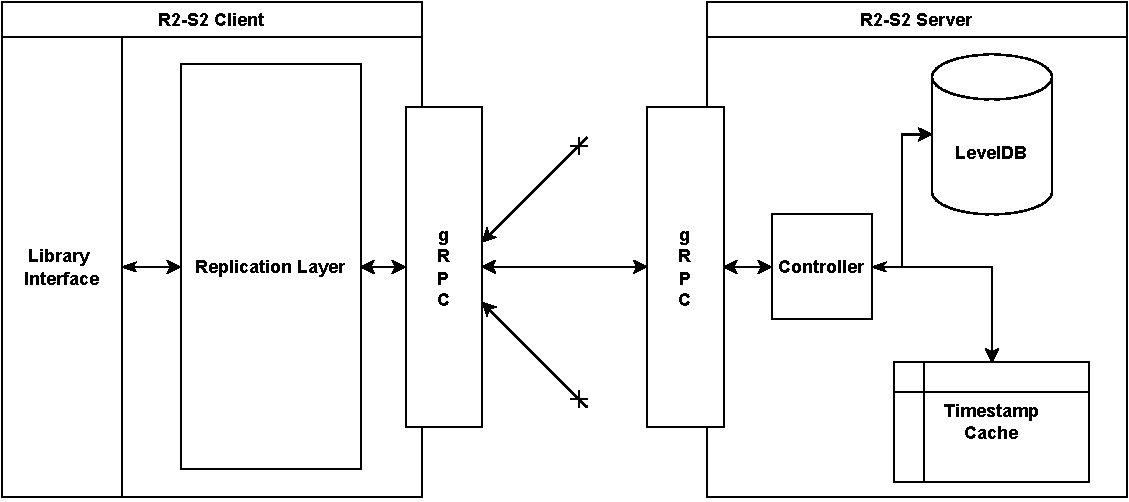
\includegraphics[width=\linewidth]{img/r2s2_arch}
    \caption{Architecture of the \ac{R2-S2}
    prototype}\label{fig:r2s2arch}
\end{figure}

The \ac{R2-S2} system is comprised of a client and several
servers, where the client is implemented as a library that
implements the replication layer and handles the connection to
and coordination of the multiple \ac{R2-S2} servers. This
replication layer also decides and coordinates the replicas to
implement the \emph{schedule} (which replicas have to synchronize
the write before replying).

Each \ac{R2-S2} server consists of an RPC controller, which
handles the interface with the client. This controller manages
the server's local \ac{KVS} (in our case,
LevelDB~\cite{leveldb}). In our prototype, we chose to implement
the ABD~\cite{abd} protocol, since its read/write interface
maches perfectly with the \ac{KVS} interface we are aiming to
implement.

\begin{figure}[ht!]
    \centering
    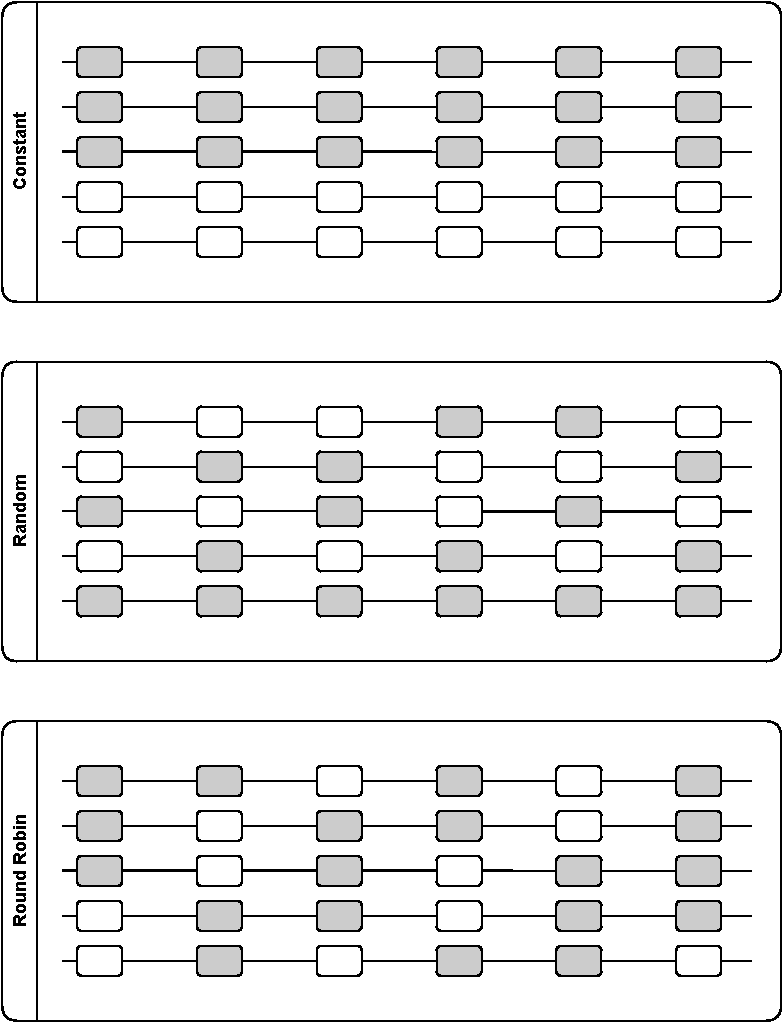
\includegraphics[width=0.75\linewidth]{img/schedules}
    \caption{Examples of valid static schedules for a
    parameterization of 5 nodes with $M_R = 2$. In each
    schedule a line represents a replica and the temporal sequence of
    objects it writes (boxes). A shaded box represents an object
    that was synchronized immediately, while a white box
    represents a batched object.}\label{fig:schedules}
\end{figure}
One relevant aspect of \ac{ABD}, and most other replication
protocols, is the notion of object versions, which are not directly supported by the
\ac{KVS} interface. Although we store the versions with the
objects for persistence, in order to order concurrent writes to the same object with
different timestamps, an in memory timestamp cache is required. This
cache is populated as needed, with synchronization on the values
to order the writes to ensure that a newer value is not
overwritten by a previous one. Additionally, this cache enables
faster queries of the object's version, which is the first phase
of an \ac{ABD} write.

The overall architecture of the \ac{R2-S2} prototype is
summarized in Figure~\ref{fig:r2s2arch}.

%%%%%%%%%%%%%%%%%%%%%%%%%%%%%%%%%%%%%%%%%%%%%%
\subsection{Scheduling}\label{ssec:schedule}
%%%%%%%%%%%%%%%%%%%%%%%%%%%%%%%%%%%%%%%%%%%%%%

As we have covered, a good schedule is crucial to realize the
performance potential of the architecture. A \emph{schedule} is a
sequence $S$, where $S_i^j$ is the mode of operation (batch and
reply, batch and wait or sync immediately) to be applied by replica
$i$ for the $j^\text{th}$ write operation. The
schedule is said to be \emph{valid} if the volatile set (i.e,
the number of batch and reply modes of operation) does not exceed
$M_R$, for every $S^j$. Thus, any valid schedule guarantees
strong persistence.

There are several approaches to scheduling. Which is preferable
is non-obvious beforehand: the schedule will be sensitive to the
particularities of the replication protocol, the deployment and
the operation load. In the preliminary evaluation in
\S~\ref{sec:r2s2evaluation} we present an
evaluation of some of the scheduling policies described
here.


At a high level, there are two types of schedules: \emph{static}
schedules, which can predetermined ahead of time, and as such
are independent of the load the system is being subjected to; and
\emph{dynamic} schedules, which are computed on the fly and as
such can be \emph{reactive} to the load and current status of the
system. In this dissertation we will focus on static schedules,
as they are simpler and sufficient to showcase the gains from the
\ac{RR} model.

\paragraph{Constant Schedule.} A constant schedule is one where
all write operations use the same modes of operation for each
replica. In other words, all $S^j$s are equal.

\paragraph{Random Schedule.} A schedule where replicas are
randomly allocated to the sync and volatile sets (based on the
sizes they need to have for the schedule to be valid).

\paragraph{Round Robin Schedule.} A schedule where the sync set
is shifted at each round. For instance, in a system with $N = 5,
M_R = 2$, replicas $0, 1, 2$ are the sync set at step $j$, and
at step $j + 1$ replicas $3, 4, 0$ become the sync set, and so
on.

Figure~\ref{fig:schedules} shows examples of different static
schedules.

%%%%%%%%%%%%%%%%%%%%%%%%%%%%%%%%%%%%%%%%%%%%%%
\subsection{Storage Layer}\label{ssec:storage}
%%%%%%%%%%%%%%%%%%%%%%%%%%%%%%%%%%%%%%%%%%%%%%

The storage layer plays a crucial role in realizing the
performance potential of the system. It needs to efficiently support
three different types of write operations, one for each of the
different baseline approaches. It will also need to support read operations
efficiently. Figure~\ref{fig:storage_layer} shows a diagram of
the storage layer and its data-structures.

An \ac{LSM-tree} is employed as the core data structure of the storage
layer, enabling the sequential writes required for batching as
well as providing reasonable read performance. There exists a
log, used to write values that need to be synced immediately, and
an in-memory batch for values that should be batched. To further speed
up reads there is an optional in-memory object cache.

\begin{figure}[t]
    \centering
    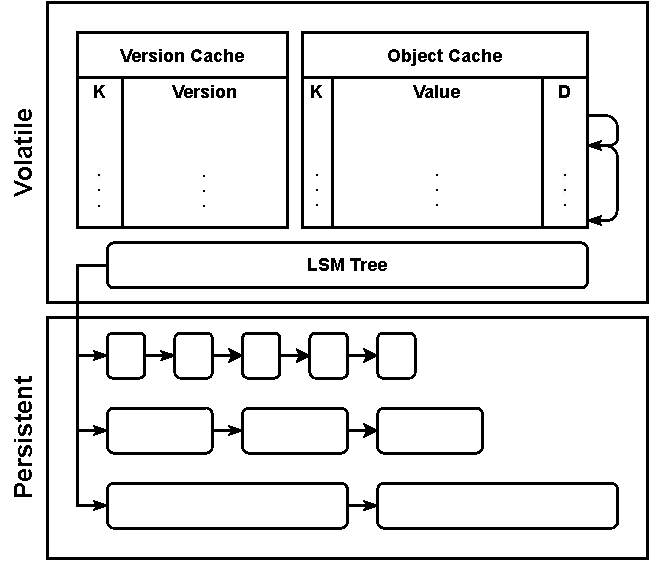
\includegraphics[width=.75\linewidth]{img/storage_layer}
    \caption{Diagram of the Storage Layer}\label{fig:storage_layer}
\end{figure}


There is an additional in-memory cache, which only stores the
object versions. This is useful because versions are a staple of
most replication protocols and several of them require reading
the current version before writing a new one. Since versions are
constant-sized and small, the capacity of the version cache can
be significantly larger than that of the object cache. This cache
is required to synchronize concurrent writes of different
versions to the same key. When the node is writing a value, it required to
check the version cache, populating it if required, where an
atomic update is executed on the version to ensure that an old
version does not override a newer version it is racing with.

With these data structures in place, the various operations
requried to implement the \ac{KVS} interface and asymmetric
syncing become quite simple. Satisfying version reads is simple:
the timestamp cache is consulted (falling back on the
\ac{LSM-tree} and log if needed). The workflow of an object read
is similar: if the object cache exists it is consulted, falling
back on the \ac{LSM-tree} and the log in the event of a miss.
Handling batch and reply writes requires placing the value
in the batch and eventually a background thread will flush the
batch into the \ac{LSM-tree}. Handling sync immediately writes
amounts to placing it in the persistent log, with this log being
compacted into the \ac{LSM-tree} at a later time by a background
thread.


%%%%%%%%%%%%%%%%%%%%%%%%%%%%%%%%%%%%%%%%%%%%%%
\section{Parameterizing the System}\label{sec:r2s2parameterization}
%%%%%%%%%%%%%%%%%%%%%%%%%%%%%%%%%%%%%%%%%%%%%%

To parameterize our system, we effectively need to choose
appropriate values for $M_R$ and $F$. We employ a data-driven
approach to this problem. Relying on real-world information about
the availability and reliability of components, we can predict
the reliability and availability of the system as a function of
$M_R$ and $F$. Choosing the adequate values becomes an exercise of
setting the desired reliability/availability and solving for $M_R$
and $F$.

The availability of the system (probability that it is available
at a particular point in time) is impacted by the availability of
the individual replicas. Let $p_c$ be the symmetric of the
availability of a replica, ie: the probability that a replica is
\emph{crashed} at a particular point in time.

The reliability (probability that the system loses data over a
given period of time) of the
system is dependent on the reliability of the underlying storage
devices and the availability of the replicas in the eager set.
Let $p_f$ be the probability that a storage device fails
(irrecoverably) in that period of time.

\emph{Note that generally, the probability of a replica crashing
is higher than that of the replica's underlying storage failing.
As such, in this discussion we assume that $p_c > p_f$.}

In order to derive the parameterization of the system, let us
begin with a simplifying assumption that all failures (both
crashes and storage device failures) are independent among all
replicas, an assumption valid for a geo-replicated deployment,
for instance. Let us first consider reliability. The probability
that all replicas in the eager set crash (and thus all the
replicas that only had the data in volatile storage lose that
data) is $p_c^{M_R}$, since $M_R$ is the size of the eager set.
To truly lose the data, the remainder of the replicas in the
write quorum would have had to suffer an irrecoverable fault in
their storage devices, which happens with probability $p^{W_Q -
M_R}$. Due to the independence of failures, we can derive the
probability that data is lost to be $p_c^{M_R} \cdot p_f^{W_Q -
M_R}$, making the reliability of the system be $1 - p_c^{M_R}
\cdot p_f^{W_Q - M_R}$. Considering availability, we know that
the system is available if a read quorum and a write quorum are
available. Due to the independence of failures, the quorums
become unavailable with probability $p_c^{R_Q}$ and $p_c^{W_Q}$,
respectively. As such, the probability that they are both
available at a given point in time is simply $1 - p_c^{\min(R_Q,
W_Q)}$.

Now let us imagine that the probability of replicas crashing
\emph{is} correlated, as is the case in a data-center deployment.
Under this assumption, an event like a power outage will cause
all replicas to crash and lose their volatile state. Therefore,
the probability of $n$ replicas crashing is the same as the
probability of a single replica crashing: $p_c$. Considering
reliability, this means that the probability of the eager set
losing its volatile state due to a crash \emph{and} the remainder
of the write quorum suffering an irrecoverable failure is $p_c
\cdot p_f^{W_Q - M_R}$. Availability is quite simpler to derive,
as if the probability of quorums of any type being unavailable is
simply $p_c$, making the availability of the system $1 - p_c$.

Table~\ref{tab:parameterization} summarizes the availability and
reliability of the system in these two scenarios.

\begin{table}[ht]
    \centering
    \caption{Availability and reliability in a geo-replicated
    deployment (uncorrelated failures) versus a data-center
    deployment (correlated failures). $R_Q$ and $W_Q$
    are the sizes of the quorums for a parameterization with $M_R$
    tolerated rollbacks and $F$ crash faults}\label{tab:parameterization}
    \begin{tabular}{|r||c|c|}
        \hline
        & \textbf{Geo-replicated} & \textbf{Datacenter} \\ \hline
        \textbf{Availability} & $1 - p_c^{\min(R_Q, W_Q)}$ & $1 - p_c$ \\ \hline
        \textbf{Reliability}  & $1 - p_c^{M_R} \cdot p_f^{W_Q - M_R}$ & $1 - p_c \cdot p_f^{W_Q - M_R}$ \\ \hline
    \end{tabular}\label{tab:parameterization}
\end{table}

It is worthwhile to compare the durability guarantees of
\ac{R2-S2} with the \ac{CFT} baselines where all replicas either sync
before replying (i.e., \emph{batch and wait} and
\emph{sync immediatelly}) or \emph{batch and reply}.

In the former case, since when replies are issued the updates are
persisted on all replicas, the reliability is independent of the
existence of crash faults (and, consequently, of the deployment
scenario). The probability of data being lost is therefore
$p_f^{Q}$, where $Q$ is the size of a quorum, making the
reliability $1 - p_f^{Q}$, which is significantly higher than
that provided by \ac{R2-S2} in either deployment scenario. This equates to this baseline
requiring less replicas to achieve the same level of reliability.

In the latter case, in which all replicas use the batch and wait
approach, the reliability can be derived from the probability of
a quorum crashing, since it is not guaranteed that the quorum
persisted the value before replying. Therefore, the
probability of data loss \emph{is} deployment sensitive. In the
geo-replicated scenario, the probability of a quorum crashing is
$p_c^Q$, whereas in the data-center scenario (where crash faults
are correlated) this probability is simply $p_c$, resulting in
a reliability of $1 - p_c^Q$ and $1 - p_c$, respectively. As
expected, these values are lower than those offered by
\ac{R2-S2}. Moreover, in the data-center scenario the reliability
is \emph{independent} of the number of replicas, since they are
likely to crash simultaneously.




%%%%%%%%%%%%%%%%%%%%%%%%%%%%%%%%%%%%%%%%%%%%%%
\section{Preliminary Evaluation}\label{sec:r2s2evaluation}
%%%%%%%%%%%%%%%%%%%%%%%%%%%%%%%%%%%%%%%%%%%%%%

In this section, we present our preliminary evaluation of the
\ac{R2-S2} prototype. We aim to answer two fundamental questions
about the approach:

\begin{enumerate}
    \item What performance benefits can be extracted using
        \emph{asymmetric synchronization}?
        (\S\ref{ssec:r2s2_eval_asym})
    \item What is the impact of different schedules in the
        performance of the \ac{R2-S2} system?
        (\S\ref{ssec:r2s2_eval_scheduling})
\end{enumerate}

%%%%%%%%%%%%%%%%%%%%%%%%%%%%%%%%%%%%%%%%%%%%%%
\subsection{Implementation}\label{sec:r2s2implementation}
%%%%%%%%%%%%%%%%%%%%%%%%%%%%%%%%%%%%%%%%%%%%%%

We implemented \ac{R2-S2} using LevelDB~\cite{leveldb} as the
underlying storage layer and our own replication layer on top of
it. This was extremely helpful since LevelDB already implements
the \ac{LSM-tree}, the persistent log and the optional object cache
out of the box, and provides for two out of the three modes of
operation: \emph{batch and reply} and \emph{sync immediately}.
We intend to implement the \emph{batch and wait} mode of
operation and incorporate it in our prototype. However, this
requires changing LevelDB to track the batches each object is
placed in and when those batches are eventually persisted.

The replication layer was implemented in Rust with the request transport
being handled by gRPC~\cite{grpc}. The \ac{R2-S2} client library
provides a shim that interacts with the replication layer that
coordinates the \ac{ABD} operations. The \ac{R2-S2} server
receives requests via gRPC and manages the timestamp cache and
its embedded LevelDB instance.

The client library was implemented in approximately 2KLoC of
Rust. The server was implemented in 400LoC. The gRPC protocol
definition is comprised of 135 LoC. All the remainder driver code
for benchmarks consists of 2KLoC of Rust.

All prototypes are open-sourced under the MIT license
and available at \url{https://gitlab.mpi-sws.org/restart-rollback}.

%%%%%%%%%%%%%%%%%%%%%%%%%%%%%%%%%%%%%%%%%%%%%%
\subsection{Methodology}\label{ssec:r2s2methodology}
%%%%%%%%%%%%%%%%%%%%%%%%%%%%%%%%%%%%%%%%%%%%%%

\begin{figure}[t]
    \centering
    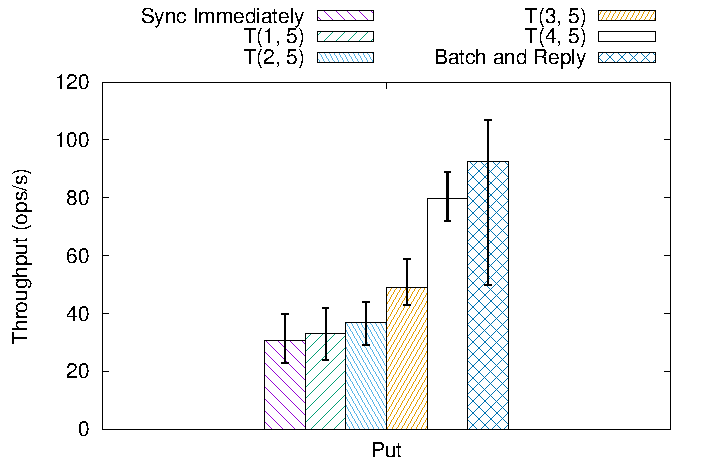
\includegraphics[width=.75\linewidth]{r2s2_results/abd_small/tput.pdf}
    \caption{Maximum throughput for different configurations.
    The \emph{batch and reply} configuration places the
    object in a batch and replies immediately, while in the
    \emph{sync immediately} configuration all replicas
    flush the object to the persistent log before replying. In
    the $T(BR, 5)$, $BR$ replicas in each write use the former
    approach, while the remaining use the
    latter.}\label{fig:r2s2_asym}
\end{figure}
\paragraph{Experimental Setup.}
We ran our experiments using 5 machines, each with an
Intel$^\text{\textregistered}$ Xeon$^\text{\textregistered}$
E-2174G processor and a 300GB Seagate Magnetic disk model
ST300MM0006, running Debian Linux version 4.19 to run the
replicas, plus one machine equipped with a
Intel$^\text{\textregistered}$ Xeon$^\text{\textregistered}$
Platinum 8260M processor running Debian Linux version 5.4 to
execute the client driver of the benchmarks.

\paragraph{Experimental Methodology.} In our result graphs, each data point represents the average
measurement throughput measurement over $60$ seconds of running
at load, using an open-loop client (i.e., a client that issues a
request asynchronously at regular time intervals to achieve the
desired load). To find the throughput in each configuration, we
ran the experiment with multiple offered loads to find the
maximum throughput point.


%%%%%%%%%%%%%%%%%%%%%%%%%%%%%%%%%%%%%%%%%%%%%%
\subsection{Asymmetric
Synchronization}\label{ssec:r2s2_eval_asym}
%%%%%%%%%%%%%%%%%%%%%%%%%%%%%%%%%%%%%%%%%%%%%%

In this experiment, we compare two baselines in the classical
\ac{CFT} model, \emph{sync immediately} and \emph{batch and reply}, with a set of \emph{threshold
configurations} ($T(BR, N)$), which vary the number of replicas that use the
batch and reply synchronization mode. Effectively, $T(0, N)$ is
the \ac{CFT} sync immediately configuration, which corresponds to
the classic system where each replica persists before replying.
Moreover $T(N, N)$ is the \ac{CFT} batch and reply configuration,
which only offers guarantees of the \emph{persistence through
replication} group, since the client obtains a reply to the write
operation before data is guaranteed to be persisted in any of the
replicas. Configurations $T(1, 5)$ and $T(2, 5)$ offer the same
persistence guarantees of $T(0, 5)$, while $T(3, 5)$ and $T(4,
5)$ offer a more subtle compromise. In these configurations there are enough replicas in the \emph{batch and reply} mode
to form a write quorum. This means that in the
event of a full system shutdown, if the other replicas that are in
fact persisting the write have not yet processed the request (or
the message was lost) the data will be lost. Nevertheless, these
(probabilistic) durability guarantees are still qualitatively
better than those of the \emph{batch and reply} baseline.

We measured the maximum throughput of each configuration using a
randomized schedule and $128KB$ objects. As we can observe in
Figure~\ref{fig:r2s2_asym}, the more replicas are
allowed to batch the higher the average throughput. We also note
the sharp increase in throughput the $T(3, 5)$ and $T(4, 5)$
configurations. This is for precisely the same reason as their
poorer durability guarantees: the \emph{batch and reply} replicas
are enough to form a write quorum, making the throughput of the
overall system significantly better.


%%%%%%%%%%%%%%%%%%%%%%%%%%%%%%%%%%%%%%%%%%%%%%
\subsection{Scheduling}\label{ssec:r2s2_eval_scheduling}
%%%%%%%%%%%%%%%%%%%%%%%%%%%%%%%%%%%%%%%%%%%%%%

Next, we compare the same two baselines in the
\ac{CFT} model, \emph{sync immediately} and \emph{batch and reply} with three \ac{RR} based quorum
configuration which aim to combine the durability of the former and
performance of the latter. Each of the \ac{RR} configurations
uses a different static schedule, as described in
Section~\ref{ssec:schedule}: constant, random and round robin.
These configurations have $M_R = 2$ and $F = 2$. This matches
both the number of tolerated crash faults of the \ac{CFT}
baselines and the total number of replicas.


\begin{figure}[t]
    \centering
    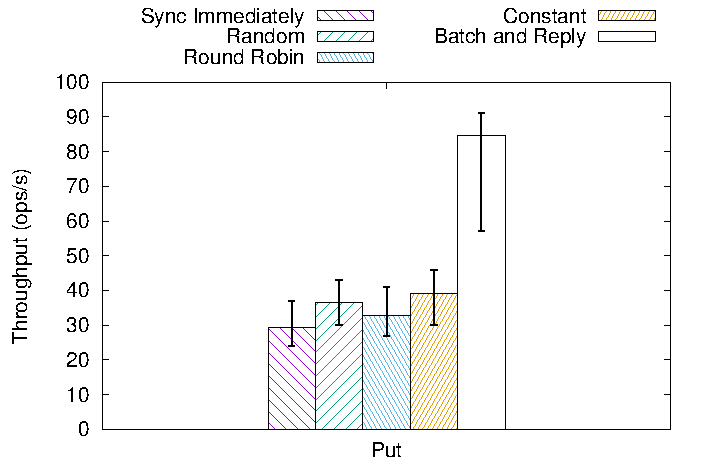
\includegraphics[width=.75\linewidth]{r2s2_results/rr_small/tput.pdf}
    \caption{Maximum throughput for different schedules.
    The \emph{batch and reply} configuration places the
    object in a batch and replies immediately, while in the
    \emph{sync immediately} configuration all replicas
    flush the object to the persistent log before replying. The
    constant schedule always synchronizes to the same $3$ of the
    $5$ replicas. The randomized schedule also synchronizes to
    $3$ replicas, but these get randomized every operation. The
    round robin schedule changes the $3$ replicas at each
    operation in a cycle.}\label{fig:r2s2_sched}
\end{figure}

We measured the maximum throughput of each configuration using  $128KB$ objects.
As we can observe in Figure~\ref{fig:r2s2_sched}, all \ac{RR}
configurations achieve throughput gains of up to $33\%$ when compared to the
\emph{sync immediately} baseline, while still achieving strong
persistence. However, there is still a large gap to the
\emph{batch and reply} baseline. Even though part of this gap is fundamentally attributed to the
lower durability guarantees offered by the \emph{batch and reply}
configuration, we also intend to bridge this implementation gap and
improve these results.

\cleardoublepage{}

\fancychapter{Conclusions and Future Work}\label{chap:conclusion}
\cleardoublepage{}

\cleardoublepage{}

% BIBLIOGRAPHY
\pdfbookmark[0]{Bibliography}{bib}
\addcontentsline{toc}{chapter}{Bibliography}
\bibliographystyle{IEEEtran}
\normalem{}
\bibliography{main}

% The following command modifies the 'emphasis' style for bibliography entries
\ULforem{}
\cleardoublepage{}

\printglossary[]
\mtcaddchapter{}

\cleardoublepage{}

\appendix
\pdfbookmark[1]{Appendix A}{appendix}
% #############################################################################
% This is Appendix A
% !TEX root = ../main.tex
% #############################################################################
\chapter{Correctness Proofs}\label{chapter:appendixA}

In this appendix, we provide the proofs of correctness for the
protocols presented in the paper. The appendix is organized as
follows:~\ref{app:quorum} presents a proof of an auxiliary
theorem regarding \ac{RR} quorum systems;~\ref{app:register}
contains a proof of correctness of the distributed register
protocol; and~\ref{app:smr} a proof of correctness of the state
machine replication protocol.

\section{\ac{RR} Quorum Systems}\label{app:quorum}

From the parametrization of \ac{RR} quorum systems derived
in Section~\ref{ssec:parameters}, we can prove a theorem that
characterizes the properties we obtain from these systems and
their quorum sizes.

\begin{theorem}\label{thrmQ}
  The quorum system defined by arbitrary subsets with the
    cardinalities in Equations
    (\ref{eq:fresh},\ref{eq:ReplSize},\ref{eq:rq_size}) is a
    Dissemination Quorum System~\cite{Malkhi:Reiter:BQS:98}.
\end{theorem}

\begin{dem}
The D-Consistency property from Definition 5.1
in~\cite{Malkhi:Reiter:BQS:98} follows from the fact that
constraint in Equation~(\ref{eq:inters}) was preserved
throughout the derivation. In particular, in the final quorum
sizes we consider, we have that the read and a write quorum
intersect in the following minimum number of replicas:

\begin{align*}
  W_Q + R_Q - N &=\\
  M_R + \Delta_W + R_Q - M_R - F - \Delta_W - \Delta_N  &=\\
  R_Q - F - \Delta_N  &=\\
  F + \min(s, M_R) + \Delta_N + \Delta_R - F - \Delta_N  &=\\
  \min(s, M_R) + \Delta_R  &
\end{align*}

\noindent which obeys the D-Consistency property because it
contains at least one non-rolled back replica ($\Delta_R >
0$), which directly implies that such a replica does not
belong to any set $B \in \cal{B}$ according to the definition
in~\cite{Malkhi:Reiter:BQS:98}.

Similarly, the D-Availability property follows from the fact that
the liveness equations were preserved throughout the
derivation. In particular, in the final quorum sizes we
consider, we have that:

\begin{align*}
    N-W_Q &=\\
    M_R + F + \Delta_W + \Delta_N - M_R - \Delta_W &=\\
    F + \Delta_N&
\end{align*}

and

\begin{align*}
    N-R_Q &=\\
    M_R + F + \Delta_W + \Delta_N - F - \min(s, M_R) - \Delta_N - \Delta_R &=\\
    M_R + \Delta_W - \Delta_R - \min(s, M_R) &\ge f'
\end{align*}
\noindent which holds given the read liveness conditions from
Equation~\ref{eq:DynRavail}.

\hfill\ensuremath{\Box}\vspace{2em}

\end{dem}

\section{Distributed Register}\label{app:register}

In this section we prove the safety of the distributed register
protocol, namely that it obeys linearizable semantics.

%% \rrnote{Algorithm highlights ---
%%     two phase read [R1, R2] + stabilize in bg /
%%     two phase write [W1, W2] + stabilize in bg /
%%     three phase cond-write: tentative-write/write/stabilize (in fg) [C1,C2,C3] /
%%     write will fail if W1 sees pre-written cond-write in progress /
%%     cond-write will abort in C1 and return fail if it sees a concurrent write or cond-write in progress /
%%     stabilize conditions: $W_Q$ of R2 ; $W_Q$ of W2 ; $W_Q$ of C2
%% }

\subsection{Specification}

The specification is simply stated as linearizability of an
object that supports read and write operations.
Linearizability states that there exists a sequential history (or
linearization) of the operations that took place in a history
of the execution of the system, such that the linearization leads
to the same outputs according to a sequential specification, and is
compatible with the real time precedence of the operations. More
precisely, this can be stated as:

\begin{itemize}
    \item[] \textbf{R-L1}: there is a total order $<$ of
        operations (reads and writes), consistent with the
        real-time invocation/reply order (meaning that if $op_1$
        returns before $op_2$ is invoked then $op_1 < op_2$)
    \item[] \textbf{R-L2}: reads return the value written by the
        most recent write according to that order.
\end{itemize}

Note that a formal proof that these properties imply linearizable semantics
can be found in~\cite{nancy-book}.

\subsection{Proof}

\paragraph{R-L1}
For proving the existence of this order, we construct the
the total order $<$ as the
lexicographic order of timestamps $<sequence number, id>$.
However, this is not yet a total order, since reads will have the same
timestamp as the operation that created the value that was returned. We
thus add the additional constraint that reads are ordered immediately
after the operation that wrote the value that was read. When several
read opearations return the same value, then we order the
reads among themselves in any total order that is compatible with the
real-time order of invocation, i.e., with the constraint that
if $read_1$ returns before $read_2$ is invoked then $read_1 < read_2$.

Given this construction, we now need to proof that this order is
consistent with the real-time precedence order, i.e., that if
operation $op_2$ is invoked after operation $op_1$ returns, then
$op_1 < op_2$.

If $op_1$ is a read, then it only concludes after either writing
back the return value to a write quorum, or reading unanimously
from a write quorum, or being signaled by the stable flag that
the value was previously present at a write quorum. Therefore,
according to Theorem~\ref{thrmQ},  a
subsequent first phase of a read or write
($op_2$) will see that timestamp at its read
quorum (or, given that timestamps grow monotonically at each replica, a higher one), and will therefore be serialized at a subsequent point in
the total order either by picking a higher timestamp for writes, or by returning the same or a higher timestamp
for reads. (In case $op_2$ is a read that returns the same timestamp,
then it obeys the required property directly by the way that $<$ is
constructed for that particular case.)

This argument also applies when $op_1$ is a write, since the second phase of each operation
also reaches a write quorum.

\paragraph{R-L2}
This follows directly from the way that the total order $<$ is
constructed. In particular, reads are serialized after the write
with the same timestamp, which is the write
that wrote the value that is returned by the
read.
%% The only problem would be if the timestamp corresponded
%% to a write that has failed, since that write
%% must not be seen. However, we prove that this is not
%% possible. Returning a failed write: writes only return fail
%% if they fail in the first phase, but in this phase they only
%% read without leaving any state at the replicas. Therefore
%% there is no possibility of a subsequent read returning a
%% failed write.

\section{State Machine Replication}\label{app:smr}

In this section, we prove the safety of the state machine
replication protocol, again using linearizable semantics as the
notion of correctness.

\subsection{Specification}

The specification is stated as linearizability of an object that
supports read and update operations. By the definition of
linearizability, there exists a sequential history
(linearization) of operations that took place in the execution of
the system. This sequential history must be compatible with the
real time order of operations and be equivalent (i.e.,\ lead to
the same outputs as) a sequential specification of the state machine.
More precisely,
it can be stated as:

\begin{enumerate}
    \item [] \textbf{SM-L1}: there is a total order $<$ of state machine operations
        (reads and updates), consistent with the real-time
        invocation/reply order (i.e.\ if $op_1$ returns before
        $op_2$ is inkoved, then $op_1 < op_2$);

      \item [] \textbf{SM-L2}: state machine operations return the value that results from the
        sequential execution of the sequence of preceding operations
        according to that order.
\end{enumerate}

As in the previous proof, the same helper theorem~\cite{nancy-book} can
be used to show that these properties imply linearizable semantics, since
it can apply to any atomic object, including a state machine.


\subsection{Proof}


\paragraph{SM-L1}
For proving the existence of this order, we construct the
the total order $<$ as the lexicographic order of slot numbers.
However, this is not yet a total order, since reads will have the same
slot number as the operation that created the value that was returned. We
thus add the additional constraint that reads are ordered immediately
after the operation that wrote the value that was read. When several
read opearations return the same value, then we order the
reads among themselves in any total order that is compatible with the
real-time order of invocation, i.e., with the constraint that
if $read_1$ returns before $read_2$ is invoked then $read_1 < read_2$.

Given this construction, we now need to proof that this order is
consistent with the real-time precedence order, i.e., that if
operation $op_2$ is invoked after operation $op_1$ returns, then
$op_1 < op_2$.

If both operations are updates, this follows from the
construction of the protocol, wherein the leader chooses the slot
position for the update and then, by collecting a super quorum of
accepts, guarantees that no subsequent update will be assigned to
that position (or a lower one), and no subsequent read will see a
lower slot number. Furthermore, for the case that the first
operation is a read, it will require a unanimous read quorum, and
additionally the replicas in this read quorum have not sent out
accept messages to other replicas. Given these protocol
mechanisms, the intersection property implied by
Theorem~\ref{thrmQ} (read quorums intersect super quorums at a
correct replica) ensure that there is no update committed to a
slot number higher than the one returned in the log of any
replica.

\paragraph{SM-L2}
This follows from the way that the total order $<$ is
constructed. In particular, (1) reads are serialized after the
update with the same slot number, which is the latest update
in the sequence of updates that leads to a state of the state machine
that corresponds to the value that is returned by the
operation, and (2) updates are serialized according to their
slot number order, with is also the order in which replicas execute those updates,
leading to outputs that are the same as the sequential specification
of the state machine.

\cleardoublepage{}

\pdfbookmark[1]{Appendix B}{appendix}
% #############################################################################
% This is Appendix B
% !TEX root = ../main.tex
% #############################################################################
\chapter{Another Appendix}
\label{chapter:appendixB}

\cleardoublepage{}

\end{document}
